%=====================================================================
%  BCaaS — Business Core as a Service
%  Rapport de projet — 3GI, Introduction aux Réseaux, S2 2025-2026
%  École Nationale Supérieure Polytechnique de Yaoundé (ENSPY)
%  Compilation : pdflatex rapport.tex  (x2 pour la table des matières)
%=====================================================================
\documentclass[11pt,a4paper,oneside]{report}

%------------------------- Encodage & langue -------------------------
\usepackage[T1]{fontenc}
\usepackage[utf8]{inputenc}
\usepackage[main=french,provide=*]{babel}
\IfFileExists{lmodern.sty}{%
  \usepackage{lmodern}%
  \IfFileExists{microtype.sty}{\usepackage{microtype}}{}%
}{}

%------------------------- Mise en page ------------------------------
\usepackage[a4paper,top=2.5cm,bottom=2.5cm,left=2.7cm,right=2.5cm]{geometry}
\usepackage{setspace}
\onehalfspacing
\usepackage{emptypage}
\newcommand{\bcaas}{BCaaS}
%------------------------- Couleurs ----------------------------------

%------------------------- Couleurs ----------------------------------
\usepackage{xcolor}
\definecolor{enspyorange}{HTML}{E8772E}
\definecolor{bcblue}{HTML}{1F3A5F}
\definecolor{bclight}{HTML}{EAF0F6}
\definecolor{bcgray}{HTML}{555555}
\definecolor{codebg}{HTML}{F6F8FA}
\definecolor{codekw}{HTML}{1F3A5F}
\definecolor{codestr}{HTML}{C7421A}
\definecolor{codecmt}{HTML}{6A737D}
% Définir la couleur primary (ajustez selon votre charte)
\definecolor{primary}{RGB}{0, 102, 204}  % Bleu
%------------------------- Graphiques & tableaux ---------------------
\usepackage{graphicx}
\usepackage{subcaption}
\usepackage{tikz}
\usetikzlibrary{
  decorations.pathreplacing,  % Pour les accolades
  positioning,                % Pour positionner les nœuds
  shapes.geometric,           % Pour des formes spécifiques
  arrows.meta                 % Pour les flèches
}
\usepackage{booktabs}
\usepackage{array}
\usepackage{longtable}
\usepackage{tabularx}
\usepackage{multirow}
\usepackage{caption}
\usepackage{float}
\captionsetup{labelfont={bf,color=bcblue},textfont={it}}
\newcolumntype{L}[1]{>{\raggedright\arraybackslash}p{#1}}
\newcolumntype{C}[1]{>{\centering\arraybackslash}p{#1}}

%------------------------- Maths -------------------------------------
\usepackage{amsmath,amssymb,amsfonts}
\usepackage{mathtools}

%------------------------- Listings (code) ---------------------------
\usepackage{listings}
\lstdefinestyle{bcstyle}{
  backgroundcolor=\color{codebg},
  basicstyle=\ttfamily\footnotesize,
  keywordstyle=\color{codekw}\bfseries,
  stringstyle=\color{codestr},
  commentstyle=\color{codecmt}\itshape,
  numberstyle=\tiny\color{bcgray},
  numbers=left, numbersep=8pt,
  showstringspaces=false,
  breaklines=true, frame=single, framerule=0pt,
  rulecolor=\color{bclight},
  xleftmargin=10pt, xrightmargin=4pt,
  aboveskip=10pt, belowskip=6pt, tabsize=2,
}
\lstset{style=bcstyle}
\lstdefinelanguage{json}{
  basicstyle=\ttfamily\footnotesize,
  stringstyle=\color{codestr},
  literate=
   *{:}{{{\color{codekw}:}}}{1}
    {\{}{{{\color{bcblue}\{}}}{1}
    {\}}{{{\color{bcblue}\}}}}{1}
    {[}{{{\color{bcblue}[}}}{1}
    {]}{{{\color{bcblue}]}}}{1},
}

%------------------------- Boîtes (analogies) ------------------------
\usepackage[most]{tcolorbox}
\newtcolorbox{analogie}[1][Analogie réseau]{
  colback=bclight, colframe=bcblue, coltitle=white,
  fonttitle=\bfseries, title={#1}, sharp corners=downhill,
  boxrule=0.6pt, left=8pt, right=8pt, top=6pt, bottom=6pt,
}
\newtcolorbox{garantie}[1][Garantie]{
  colback=enspyorange!8, colframe=enspyorange, coltitle=white,
  fonttitle=\bfseries, title={#1}, sharp corners=downhill,
  boxrule=0.6pt, left=8pt, right=8pt, top=6pt, bottom=6pt,
}
\newtcolorbox{question}[1][Question directrice]{
  colback=white, colframe=bcblue, coltitle=white,
  fonttitle=\bfseries, title={#1},
  boxrule=0.8pt, left=8pt, right=8pt, top=6pt, bottom=6pt,
}

%------------------------- Titres (titlesec) -------------------------
\usepackage{titlesec}
\titleformat{\chapter}[display]
  {\sffamily\bfseries\color{bcblue}}
  {\filright\Large\color{enspyorange}\MakeUppercase{\chaptertitlename}\ \thechapter}
  {8pt}{\Huge}
\titlespacing*{\chapter}{0pt}{10pt}{30pt}
\titleformat{\section}{\sffamily\Large\bfseries\color{bcblue}}{\thesection}{0.6em}{}
\titleformat{\subsection}{\sffamily\large\bfseries\color{bcblue!85}}{\thesubsection}{0.6em}{}
\titleformat{\subsubsection}{\sffamily\normalsize\bfseries\color{bcgray}}{\thesubsubsection}{0.6em}{}

%------------------------- En-têtes / pieds --------------------------
\usepackage{fancyhdr}
\pagestyle{fancy}
\fancyhf{}
\setlength{\headheight}{14pt}
\fancyhead[L]{\footnotesize\itshape\color{bcgray} BCaaS — Business Core as a Service}
\fancyhead[R]{\footnotesize\itshape\color{bcgray} 3GI — 2025-2026}
\fancyfoot[C]{\thepage}
\renewcommand{\headrulewidth}{0.4pt}
\renewcommand{\headrule}{\hbox to\headwidth{\color{enspyorange}\leaders\hrule height \headrulewidth\hfill}}

%------------------------- Liens -------------------------------------
\usepackage[hidelinks]{hyperref}
\hypersetup{
  colorlinks=true, linkcolor=bcblue, citecolor=enspyorange,
  urlcolor=enspyorange, pdftitle={BCaaS — Business Core as a Service},
  pdfauthor={Groupe BizCore — 3GI ENSPY},
}
\usepackage{enumitem}
\setlist{itemsep=2pt,topsep=4pt}

%------------------------- Commande figure placeholder ---------------
\newcommand{\figplaceholder}[2]{%
  \begin{center}
  \fcolorbox{bcblue}{bclight}{%
    \begin{minipage}[c][#2][c]{0.85\linewidth}\centering
      \sffamily\color{bcgray}\textbf{[ FIGURE À INSÉRER ]}\\[4pt]
      \footnotesize #1
    \end{minipage}}
  \end{center}}

%=====================================================================
\begin{document}
\sloppy

	
	%===================== PAGE DE GARDE ===============================
\begin{titlepage}
	
	% === RÉDUIRE LES MARGES UNIQUEMENT ICI ===
	\newgeometry{top=1.2cm, bottom=1.2cm, left=1.5cm, right=1.5cm}
	
	% === EN-TÊTE BILINGUE AVEC LOGO CENTRÉ ===
	\begin{center}
		\begin{tabular}{m{0.4\textwidth} m{0.15\textwidth} m{0.4\textwidth}}
			\begin{flushleft}
				\begin{center}
					{\small
						{République du Cameroun}\\
						\textit{Paix -- Travail -- Patrie}\\
						---------------\\
						{Université de Yaoundé I}\\
						---------------\\
						École Nationale Supérieure Polytechnique de Yaoundé\\
						{(ENSPY)}\\
						---------------\\
						Département de Génie Informatique
					}
				\end{center}
			\end{flushleft}
			&
			\centering
			
\includegraphics[width=2.5cm]{figures/logopo-rbg.png}
			&
			\begin{flushright}
				\begin{center}
					{\small
						{Republic of Cameroon}\\
						\textit{Peace -- Work -- Fatherland}\\
						---------------\\
						{University of Yaoundé I}\\
						---------------\\
						National Advanced School of Engineering of Yaoundé\\
						{(NASEY)}\\
						---------------\\
						Department of Computer Engineering
					}
				\end{center}
			\end{flushright}
		\end{tabular}
	\end{center}
	
	\vspace{0.2cm}
	
	% --- Trait décoratif ---
	{\color{bcblue}\rule{\linewidth}{1.2pt}}
	\vspace{0.1cm}
	{\color{enspyorange}\rule{\linewidth}{0.5pt}}
	
	\vspace{0.3cm}
	
	% --- Titre RAPPORT DE PROJET ---
	\begin{center}
		{\Large \bfseries \color{bcblue} Rapport de projet}
		
	
		{\sffamily\bfseries\color{enspyorange}\fontsize{34}{38}\selectfont Business Core as a Service\par}
		\vspace{0.1cm} 
		{ \itshape \color{gray!60} Une infrastructure générique de gestion des métiers\\[0.05cm]
			inspirée de l'ingénierie des protocoles réseaux}
	\end{center}
	
	% --- Trait décoratif ---
	{\color{enspyorange}\rule{\linewidth}{0.5pt}}
	\vspace{0.1cm}
	{\color{bcblue}\rule{\linewidth}{1.2pt}}
	
	\vspace{0.3cm}
	
	% --- GROUPE 3 ---
	\begin{center}
		{\large \bfseries \color{enspyorange} \textsc{Groupe 3}}
	\end{center}
	
	\vspace{0.1cm}
	
	% --- Auteurs ---
	\begin{center} 
		\vspace{0.15cm}
		\renewcommand{\arraystretch}{1.15}
		\begin{tabular}{l c c}
			\toprule[0.6pt]
			\textbf{Nom \& Prénom(s)} & \textbf{Matricule} & \textbf{Participation (\%)} \\
			\midrule
			ETCHOME Chris Manuel Loîc                 & 23P393 & 100 \\
			KEMDA DEMANOU Jean Loïc        & 22P356 & 100 \\
			KENNE DIHA Ange Léa            & 23P566 & 70\\
			
			KONGNI TCHINDA Jude Roland     & 23P349 & 70\\
            KOTCHAP TINGA Blessing         & 23P350 & 60 \\
			MBA BELA Océanne               & 23P518 & 70 \\
            
			\bottomrule[0.6pt]
		\end{tabular}
	\end{center}
	
	\vspace{0.3cm}
	
	% --- Encadrement (à droite) ---
	\begin{flushright}
		{ \bfseries \color{bcblue} \large Sous la supervision de :}
		
		\vspace{0.05cm}
		{  Pr. Dr Ing. \textbf{Thomas Djotio Ndié}}
		
		\vspace{0.2cm}
		
		{  \bfseries \color{bcblue} Assistant :}
		
		\vspace{0.05cm}
		{ \textbf{Juslin KUTCHE NEGOUE}}
		
		\vspace{0.05cm}
		{\small MSc, PhD Student}
	\end{flushright}
	
	\vfill
	
	% --- Pied de page ---
	\begin{center}
		{\small Année académique 2025-2026} 
	\end{center}
	
	% === RESTAURER LES MARGES ORIGINALES ===
	\restoregeometry
	
\end{titlepage}

\pagenumbering{roman}

%=====================  RÉSUMÉ  ======================================
\chapter*{Résumé}
\addcontentsline{toc}{chapter}{Résumé}
\markboth{Résumé}{Résumé}

Ce rapport présente la conception, l'implémentation et le déploiement de \textbf{BCaaS}
(\emph{Business Core as a Service}), une plateforme générique \emph{multi-tenant}
dédiée à la gestion standardisée des processus métier. Le projet s'inscrit dans le cadre
du cours d'Introduction aux Réseaux de la troisième année de Génie Informatique de
l'École Nationale Supérieure Polytechnique de Yaoundé. L'idée centrale consiste à modéliser un système d'information métier en s'appuyant rigoureusement sur les concepts de l'ingénierie des protocoles réseaux : pile de couches,
encapsulation, routage, adressage, qualité de service, et séparation des plans de contrôle
et de données. Cette analogie formelle, loin d'être une simple métaphore pédagogique,
structure l'ensemble des décisions architecturales : un \emph{tenant} y joue le rôle d'un
VLAN, une demande de service celui d'un paquet, et la facture celui d'un accusé de
réception. La solution livrée repose sur Spring Boot 3.5 / Java 21, PostgreSQL avec Liquibase,
Spring Security avec authentification JWT et isolation multi-tenant par colonne
\texttt{tenant\_id}, et SpringDoc OpenAPI pour la documentation automatique de l'API.
Le domaine compte quinze entités et l'API expose environ quatre-vingt-cinq points de
terminaison REST validés par cent cinquante-deux tests automatisés. Un frontend Next.js
(site vitrine et tableau de bord d'administration) complète l'ensemble. L'API est déployée
sur Render et la documentation sur Vercel.

\vspace{6pt}
\noindent\textbf{Mots-clés :} Business Core, multi-tenant, protocoles réseaux, modèle OSI,
encapsulation, Spring Boot, API REST, JWT, Next.js, architecture hexagonale.

%=====================  ABSTRACT  ====================================
\chapter*{Abstract}
\addcontentsline{toc}{chapter}{Abstract}
\markboth{Abstract}{Abstract}

This report presents the design, implementation and deployment of \textbf{BCaaS}
(\emph{Business Core as a Service}), a generic \emph{multi-tenant} platform dedicated to
the standardized management of business processes. The project was carried out within the
Introduction to Networks course of the third year of Computer Engineering at the National
Advanced School of Engineering of Yaoundé.The core idea is to model a business information system by rigorously relying on the
concepts of network protocol engineering: layered stack, encapsulation, routing,
addressing, quality of service, and the separation of control and data planes. This formal
analogy is not a mere pedagogical metaphor; it drives every architectural decision: a
\emph{tenant} plays the role of a VLAN, a service request that of a packet, and an
invoice that of an acknowledgement signal. The delivered solution is built on Spring Boot 3.5 / Java 21, PostgreSQL with Liquibase,
Spring Security with JWT authentication and \texttt{tenant\_id}-based multi-tenant
isolation, and SpringDoc OpenAPI for automatic API documentation. The domain comprises
fifteen entities and the API exposes roughly eighty-five REST endpoints validated by one
hundred and fifty-two automated tests. A Next.js frontend (public showcase site and
administration dashboard) completes the system. The API is deployed on Render and the
documentation on Vercel.

\vspace{6pt}
\noindent\textbf{Keywords:} Business Core, multi-tenant, network protocols, OSI model,
encapsulation, Spring Boot, REST API, JWT, Next.js, hexagonal architecture.

%=====================  TOC / FIGURES / TABLES =======================
\cleardoublepage
\tableofcontents
\cleardoublepage
\listoffigures
\cleardoublepage
\listoftables

%=====================  ABRÉVIATIONS =================================
\chapter*{Liste des abréviations}
\addcontentsline{toc}{chapter}{Liste des abréviations}
\markboth{Liste des abréviations}{Liste des abréviations}

\renewcommand{\arraystretch}{1.3}
\begin{longtable}{L{3.2cm} L{11cm}}
\toprule
\textbf{Sigle} & \textbf{Signification} \\
\midrule \endhead
BCaaS & Business Core as a Service \\
BaaS  & Business as a Service \\
API   & Application Programming Interface \\
REST  & Representational State Transfer \\
JWT   & JSON Web Token \\
RBAC  & Role-Based Access Control \\
DDD   & Domain-Driven Design \\
DTO   & Data Transfer Object \\
FSM   & Finite State Machine (machine à états finis) \\
OSI   & Open Systems Interconnection \\
TCP/IP& Transmission Control Protocol / Internet Protocol \\
VLAN  & Virtual Local Area Network \\
SDN   & Software-Defined Networking \\
QoS   & Quality of Service \\
SLA   & Service-Level Agreement \\
MCD   & Modèle Conceptuel de Données \\
MLD   & Modèle Logique de Données \\
UML   & Unified Modeling Language \\
PWA   & Progressive Web App \\
SSR   & Server-Side Rendering \\
CdS   & Consommateur de Service \\
FdS   & Fournisseur de Service \\
KPI   & Key Performance Indicator \\
RLS   & Row-Level Security \\
UUID  & Universally Unique Identifier \\
\bottomrule
\end{longtable}

\cleardoublepage
\pagenumbering{arabic}

%#####################################################################
%  Les chapitres sont inclus ci-dessous.
%#####################################################################
\chapter{Introduction générale}

\section{Contexte du projet}

%Dans le domaine du génie logiciel, chaque nouveau projet métier qu'il %s'agisse d'une
%pharmacie, d'une agence immobilière, d'un cabinet médical, d'une auto-école %ou d'une
%école reconstruit invariablement les mêmes fondations : gestion des acteurs, des
%ressources, des règles, des workflows, des notifications et de la traçabilité. Cette
%duplication systématique représente un gaspillage considérable en temps de développement,
%en coût de maintenance et en cohérence architecturale.

%Parallèlement, l'ingénierie des réseaux a résolu depuis des décennies un problème
%structurellement similaire : faire communiquer de façon fiable, sécurisée et interopérable
%des entités hétérogènes sur une infrastructure partagée. Le modèle OSI et la suite TCP/IP
%proposent une décomposition en couches aux responsabilités clairement délimitées, un
%mécanisme d'encapsulation des données, un adressage précis des destinataires, une qualité
%de service différenciée, et une séparation nette entre plan de contrôle et plan de données.

%Le présent projet a pour objectif pédagogique est précisément d'établir un
%\emph{lien formel} entre les concepts du domaine des réseaux et ceux d'un domaine métier.
%BCaaS constitue le \emph{noyau générique} (\emph{Business Core}) sur lequel les autres
%instances métier de la promotion (pharmacie, immobilier, tourisme, médical, etc.) peuvent
%se greffer.

L’application métier est par définition une application développée selon des besoins métier. Elle permet de faciliter la gestion des activités d’une entreprise en simplifiant les tâches tout en automatisant les process. Depuis l’essor de la digitalisation, télétravail et BYOD (Bring your own device), la tendance est aux applications développées selon les spécificités de chaque métier ou chaque profil. Ainsi dans un contexte où les organisations multiplient ces applications métier spécifiques à chaque secteur d'activité, chaque nouveau projet métier, qu'il s'agisse d'une pharmacie, d'une agence immobilière, d'un cabinet médical, d'une auto-école ou d'une école, elle reconstruit invariablement les mêmes fondations : gestion des acteurs, des ressources, des règles métier, des workflows, ou des mécanismes d'audit, les mêmes briques logicielles sont reconstruites à chaque nouveau projet.\\

Parallèlement, l'ingénierie des réseaux informatiques a depuis longtemps résolu un problème structurellement similaire : permettre à des flux de données hétérogènes de circuler de manière fiable, sécurisée et interopérable à travers une infrastructure partagée. Le modèle OSI et la suite TCP/IP proposent une décomposition en couches aux responsabilités clairement délimitées, un
mécanisme d'encapsulation des données, un adressage précis des destinataires, une qualité
de service différenciée, et une séparation nette entre plan de contrôle et plan de données.Les principes qui gouvernent les réseaux séparation des responsabilités en couches, encapsulation des données, routage, contrôle de la qualité de service constituent une référence éprouvée pour structurer des systèmes complexes. Les principes qui gouvernent les réseaux séparation des responsabilités en couches, encapsulation des données, routage, contrôle de la qualité de service constituent une référence éprouvée pour structurer des systèmes complexes. C'est dans ce contexte que s'inscrit le concept de Business Core as a Service (BCaaS) : une infrastructure générique de gestion des métiers inspirée de l'ingénierie des protocoles réseaux.

\section{Problème}

%Le problème adressé est celui de la \textbf{ré-implémentation perpétuelle des fondations
%métier}. Concrètement :
%\begin{itemize}
  %\item la fragmentation des outils de gestion entre métiers, sans interopérabilité ;
  %\item l'absence de standardisation des concepts récurrents (acteur, service, ressource,
   %     règle métier, facture) ;
  %\item la difficulté de mise en relation entre un consommateur de service (CdS) et un
   %     fournisseur de service (FdS) ;
  %\item le manque de traçabilité du cycle de vie des prestations ;
  %\item la gestion manuelle et non auditée de la facturation.
%\end{itemize}

Les applications métier (gestion de pharmacie, d'agence immobilière, de cabinet médical, d'auto-école, d'école, etc.) reposent toutes sur les mêmes fondations : gestion des acteurs, des ressources, des règles métier, des workflows et de l'audit. Pourtant, ces briques communes sont reconstruites à chaque nouveau projet, sans méthode de conception réutilisable ni séparation claire des responsabilités, ce qui rend ces applications difficiles à faire évoluer et peu adaptées à une utilisation par plusieurs clients (tenants) sur une même infrastructure.\\

Le problème qui se pose est donc le suivant : concevoir une infrastructure métier générique, modulaire et multitenant, en s'appuyant sur les principes de structuration en couches, d'encapsulation et de routage déjà éprouvés par l'ingénierie des protocoles réseaux

\section{Problématique}

\begin{question}
Comment concevoir un noyau métier générique, réutilisable et configurable qui permette à
n'importe quelle instance métier de fonctionner sans reconstruire les fondations, en
s'appuyant formellement sur les concepts de l'ingénierie des protocoles réseaux ?
\end{question}

Cette question directrice se décline en sous-questions a savoir : \\
%quels concepts réseaux peut-on
%mettre en correspondance avec quels composants métier ? Comment garantir l'isolation des
%données de clients distincts sur une infrastructure partagée, à la manière d'un VLAN ?
%Comment formaliser le « protocole » d'échange d'un cas métier concret ?

%\begin{enumerate}
    \textbf{Sur la structuration en couches:} Comment décomposer un Business Core en couches aux responsabilités clairement délimitées, à l'image du modèle OSI, de sorte que chaque couche masque sa complexité aux couches voisines tout en leur offrant des services bien définis ?

    \textbf{Sur l'encapsulation des échanges:}Comment séparer, au sein d'un même message métier, les métadonnées de routage et de contexte (identité du tenant, de l'acteur, traçabilité) du contenu métier proprement dit, afin qu'un service puisse appliquer les politiques communes sans connaître l'ensemble de l'application ?

    \textbf{Sur le routage et l'identification:}Comment résoudre, pour chaque requête entrante, le tenant, le domaine métier et le service cible auquel elle doit être acheminée, de manière analogue à l'adressage IP dans un réseau ?

    \textbf{Sur l'isolation multitenant:}Comment garantir qu'une infrastructure partagée entre plusieurs clients préserve une isolation stricte de leurs données et de leurs processus, à l'image de la virtualisation réseau (VLAN, namespace) ?

    \textbf{Sur la séparation gouvernance/exécution:} Comment distinguer, au sein du Business Core, un plan de contrôle (configuration des règles, des tenants, des SLA) d'un plan de données (exécution effective des transactions métier), afin de permettre une reconfiguration du système sans interruption de service ?
%\end{enumerate}

  
\section{Objectifs}

\subsection{Objectif général}
Concevoir et réaliser une plateforme générique multi-tenant de gestion des métiers,
architecturée selon une analogie rigoureuse avec la pile protocolaire réseau.

\subsection{Objectifs spécifiques}
\begin{enumerate}
  \item Établir une analogie formelle et rigoureuse entre les concepts réseaux (couches
        OSI, encapsulation, routage, QoS, multi-tenant) et les composants d'une
        architecture métier générique.
  \item Définir une pile protocolaire métier en cinq couches (infrastructure, transport et messaging,         tenant et routage, contexte et politique, capacités métier), où chaque couche assure une              fonction précise et masque sa complexité aux couches voisines.%Concevoir une architecture modulaire multi-tenant, lisible à travers une pile
        %protocolaire métier en cinq couches.
  \item Implémenter une API REST de provisionnement de tenants reposant sur un modèle de
        données générique configurable.
        
  \item Proposer une stratégie de multitenant et d'isolation garantissant la séparation logique des           données et des processus entre les différents clients partageant la même infrastructure.
        %Sécuriser les échanges par authentification JWT et contrôle d'accès basé sur les
        %rôles (RBAC), avec isolation stricte par tenant.
  \item Documenter et exposer l'API via Swagger UI, et déployer la solution
        (API et documentation) sur le cloud.
  \item Développer un frontend Next.js comprenant un site vitrine et la documentation détaillée de l'API REST. \end{enumerate}

\section{Méthodologie}

%Le projet a été conduit de manière incrémentale, organisée en \emph{sprints} successifs
%assortis de critères de priorité (P0 : indispensable ; P1 : important). L'architecture
%retenue est une \textbf{architecture hexagonale} (ports et adaptateurs) combinée au
%\textbf{Domain-Driven Design} (DDD), afin de préserver l'indépendance du domaine métier
%vis-à-vis des détails techniques. Chaque étape a fait l'objet d'une validation explicite
%(modélisation Merise, diagrammes UML, audits de code, tests automatisés) avant de passer
%à la suivante.
Pour répondre aux objectifs fixés, notre démarche s'appuie sur une progression en quatre étapes successives.\\

La première étape consiste à établir une analyse comparative entre les concepts fondamentaux de l'ingénierie des réseaux (modèle OSI, adressage IP, encapsulation, contrôle de la qualité de service) et les besoins propres à une architecture métier générique. Cette étape pose les bases conceptuelles du projet en faisant correspondre chaque mécanisme réseau à un équivalent métier.\\

La deuxième étape traduit cette analyse en un modèle mathematique d'une part et architectural d'autre part, structuré selon une pile de cinq couches respectant les principes d'abstraction et d'encapsulation. Chaque couche est définie avec ses responsabilités propres et ses interfaces vis-à-vis des couches voisines.\\
       
La troisième étape regroupe la conception, l'implémentation et les tests du système. Elle consiste d'abord à appliquer l'architecture définie à un scénario métier précis (santé, transport, logistique, etc.), en modélisant un flux d'échange complet, de la requête initiale à la propagation des événements. Cette conception est ensuite mise en œuvre à travers le développement des composants du Business Core, incluant la stratégie d'isolation multitenant garantissant la séparation des données entre clients. Enfin, des tests sont menés pour valider le bon fonctionnement de l'architecture, vérifier la cohérence des contrats d'échange entre services et s'assurer du respect des exigences de sécurité et d'isolation.\\

La quatrième étape ouvre une réflexion sur les perspectives d'évolution du Business Core, à travers la mise en place de mécanismes d'observabilité et de qualité de service, ainsi que l'identification des pistes d'extension possibles : ajout de nouveaux domaines métier, enrichissement des règles de gouvernance, ou amélioration de la résilience du système face à la montée en charge.




\section{Structure du document}

Le rapport est organisé comme suit. Le chapitre~\ref{chap:etat-de-lart} dresse l'état de l'art.
Le chapitre~\ref{chap:analogie} formalise l'analogie réseau--métier, cœur conceptuel du
projet, et y présente la pile protocolaire en cinq couches. Le chapitre~\ref{chap:besoins}
spécifie les besoins fonctionnels et non fonctionnels. Le chapitre~\ref{chap:math} propose
une modélisation mathématique du système. Les chapitres~\ref{chap:archi}
et~\ref{chap:donnees} détaillent la conception architecturale et la conception des données.
Le chapitre~\ref{chap:impl} décrit l'implémentation technique, le
chapitre~\ref{chap:protocole} le protocole d'échange d'un cas métier, et le
chapitre~\ref{chap:observ} la traçabilité et l'observabilité. Le
chapitre~\ref{chap:frontend} traite du frontend et du déploiement, le
chapitre~\ref{chap:tests} des tests et de la validation, et le chapitre~\ref{chap:gestion}
de la gestion de projet. Le chapitre~\ref{chap:perspectives} expose les perspectives
d'amélioration, avant la conclusion générale (chapitre~\ref{chap:conclusion}).

% ============================================================
%  CHAPITRE 2 — État de l'art
%  À inclure dans le document principal avec :
%    \input{chapitre2}   ou   \include{chapitre2}
%
%  Packages supposés chargés dans le main :
%    \usepackage[french]{babel}
%    \usepackage[utf8]{inputenc}
%    \usepackage[T1]{fontenc}
%    \usepackage{booktabs}
%    \usepackage{array}
%    \usepackage{tabularx}
%    \usepackage{xcolor}
%    \usepackage{hyperref}
%    \usepackage{geometry}
%    \usepackage{enumitem}
%    \usepackage{parskip}       % ou gestion manuelle des espacements
% ============================================================

\chapter{État de l'art}
\label{chap:etat-de-lart}

Ce chapitre situe le projet BCaaS (\textit{Business Core as a Service}) dans son paysage
scientifique et technique. Il ne s'agit pas simplement de lister des concepts existants,
mais de montrer comment chacun d'eux contribue à la conception de BCaaS et en quoi leur
combinaison constitue une approche originale. Nous passerons successivement en revue les
modèles en couches issus des réseaux informatiques, les stratégies d'architecture
multi-tenant, le paradigme \textit{as-a-Service} et son extension au niveau métier, les
principes de l'architecture hexagonale et du \textit{Domain-Driven Design}, avant de
conclure en positionnant la contribution spécifique de BCaaS par rapport à cet état de
l'art.

% ------------------------------------------------------------
\section{Modèles en couches : OSI et TCP/IP}
\label{sec:osi-tcpip}

% ---- 2.1.1 -------------------------------------------------
\subsection{Le modèle OSI}
\label{subsec:osi}

Le modèle OSI (\textit{Open Systems Interconnection}), normalisé par l'ISO sous la
référence ISO/IEC~7498-1~\cite{iso7498}, est un cadre de référence conceptuel qui décompose
la communication entre deux systèmes informatiques en sept couches aux responsabilités
strictement délimitées. Chaque couche remplit une fonction précise et ne communique
directement qu'avec les couches immédiatement adjacentes, sans connaître les détails de
fonctionnement des autres.

Les sept couches, de la plus basse à la plus haute, sont les suivantes :

\begin{description}[leftmargin=2.5cm, labelwidth=2.2cm, style=nextline]
  \item[\textbf{Couche~1 Physique}]
    Transmission des bits bruts sur le médium (câble, fibre, ondes radio). Elle définit
    les niveaux de tension, les fréquences et les connecteurs physiques.

  \item[\textbf{Couche~2 Liaison}]
    Organisation des bits en trames, détection (voire correction) d'erreurs de
    transmission, et contrôle d'accès au médium partagé (protocoles Ethernet, Wi-Fi).

  \item[\textbf{Couche~3 Réseau}]
    Adressage logique (adresses IP) et routage des paquets entre réseaux différents.
    C'est la couche qui permet à un paquet de traverser plusieurs réseaux intermédiaires
    pour atteindre sa destination.

  \item[\textbf{Couche~4 Transport}]
    Communication de bout en bout entre processus, avec ou sans garantie de fiabilité.
    TCP assure la livraison ordonnée et sans perte~; UDP privilégie la rapidité au
    détriment de cette garantie.

  \item[\textbf{Couche~5 Session}]
    Établissement, maintien et terminaison des sessions de dialogue entre deux
    applications.

  \item[\textbf{Couche~6 Présentation}]
    Mise en forme des données (encodage des caractères, compression, chiffrement) afin
    que les applications puissent se comprendre indépendamment de leurs représentations
    internes.

  \item[\textbf{Couche~7 Application}]
    Interface directe avec les logiciels utilisateurs. C'est ici que résident les
    protocoles applicatifs tels que HTTP, SMTP, FTP ou DNS.
\end{description}

Le principe central du modèle OSI est l'\textbf{encapsulation} : lorsqu'une donnée
descend la pile d'émission, chaque couche y ajoute un en-tête (et parfois un pied de
trame) contenant les informations de contrôle nécessaires à son homologue sur la machine
distante. À réception, la pile est parcourue en sens inverse~: chaque couche lit et retire
son en-tête avant de passer les données à la couche supérieure. Ce mécanisme garantit une
séparation complète des responsabilités~: chaque couche ignore le contenu des données
qu'elle transporte et ne se préoccupe que de sa propre fonction.

\begin{table}[ht]
  \centering
  \caption{Les sept couches OSI et leurs analogies dans BCaaS}
  \label{tab:osi-bcaas}
  \renewcommand{\arraystretch}{1.3}
  \begin{tabularx}{\textwidth}{>{\centering\bfseries}p{1.2cm}
                               >{\bfseries}p{2.4cm}
                               >{\raggedright\arraybackslash}X
                               >{\raggedright\arraybackslash}X}
    \toprule
    \textbf{N°} & \textbf{Couche} & \textbf{Rôle principal} & \textbf{Analogie BCaaS} \\
    \midrule
    7 & Application   & Interface avec l'utilisateur final                    & API métier exposée aux clients \\
    6 & Présentation  & Encodage, chiffrement, compression                    & Sérialisation JSON/XML, tokens JWT \\
    5 & Session       & Gestion des sessions de communication                 & Gestion des sessions utilisateur \\
    4 & Transport     & Fiabilité, contrôle de flux (TCP/UDP)                 & File d'attente, retry, transactions \\
    3 & Réseau        & Adressage et routage inter-réseaux                    & Routage multi-tenant, isolation VLAN \\
    2 & Liaison       & Détection d'erreurs, accès au médium                  & Validation des données, contraintes DB \\
    1 & Physique      & Transmission binaire sur le médium                    & Infrastructure serveur, cloud \\
    \bottomrule
  \end{tabularx}
\end{table}

% ---- 2.1.2 -------------------------------------------------
\subsection{La suite TCP/IP}
\label{subsec:tcpip}

La suite de protocoles TCP/IP, développée par le Département de la Défense américain dans
les années~1970 et standardisée au sein des RFC (\textit{Request For Comments}), adopte
une approche plus pragmatique en condensant les sept couches OSI en quatre niveaux~:
accès réseau (couches~1-2), Internet (couche~3), transport (couche~4) et application
(couches~5-7). C'est ce modèle qui régit le fonctionnement d'Internet depuis son origine.

TCP/IP conserve les mêmes idées directrices que le modèle OSI — adressage, routage,
fiabilité, contrôle de flux — mais en simplifiant leur mise en œuvre. Son adoption
universelle a été rendue possible par sa flexibilité~: l'adressage IP, notamment avec
IPv6, permet d'identifier de manière unique chaque appareil connecté à l'échelle mondiale.

% ---- 2.1.3 -------------------------------------------------
\subsection{Intérêt méthodologique pour BCaaS}
\label{subsec:osi-bcaas}

Au-delà de leur application aux réseaux informatiques, ces modèles présentent un intérêt
méthodologique fondamental pour la conception logicielle. Trois principes sont
particulièrement transposables~:

\begin{description}[leftmargin=0.5cm]
  \item[\textbf{Séparation des préoccupations par couches} (\textit{Separation of
    Concerns})]
    Chaque module ou composant logiciel est responsable d'une et d'une seule fonction. Ce
    principe réduit la complexité, facilite les tests unitaires et rend les composants
    remplaçables indépendamment.

  \item[\textbf{Encapsulation progressive du contexte}]
    Chaque couche enrichit les données d'informations supplémentaires (métadonnées,
    identifiants, contexte de sécurité) sans que les couches adjacentes n'aient à
    connaître ces détails. En logiciel, cela correspond à l'enrichissement d'un objet
    métier à mesure qu'il traverse les différentes couches d'une application (validation,
    transformation, persistance).

  \item[\textbf{Adressage explicite des destinataires}]
    Dans TCP/IP, une adresse IP et un port identifient sans ambiguïté la destination d'un
    paquet. En architecture multi-tenant, l'identifiant du tenant (\texttt{tenant\_id})
    joue un rôle analogue~: il adresse chaque requête vers le bon contexte de données et
    de règles métier.
\end{description}

C'est cette transposition que BCaaS exploite explicitement~: la pile applicative métier
est conçue comme une pile protocolaire, avec des couches aux responsabilités distinctes,
des mécanismes d'encapsulation du contexte (tenant, utilisateur, droits) et un adressage
explicite par \texttt{tenant\_id}.

% ------------------------------------------------------------
\section{Architectures multi-tenant}
\label{sec:multi-tenant}

% ---- 2.2.1 -------------------------------------------------
\subsection{Définition et enjeux}
\label{subsec:multitenant-def}

Une application est dite \textbf{multi-tenant} (multi-locataire) lorsqu'une seule instance
logicielle sert simultanément plusieurs organisations ou clients distincts (les
\textit{tenants} ) tout en garantissant l'isolation totale de leurs données et
configurations. Ce modèle s'oppose au modèle multi-instance, où chaque client dispose de
sa propre installation du logiciel~\cite{multitenant}.

Les enjeux du multi-tenant sont multiples et parfois contradictoires~:

\begin{description}[leftmargin=0.5cm]
  \item[\textbf{Isolation des données}]
    Un tenant ne doit jamais pouvoir accéder, même accidentellement, aux données d'un
    autre. Cette exigence est à la fois technique (partitionnement physique ou logique) et
    réglementaire (RGPD, normes sectorielles).

  \item[\textbf{Performance et scalabilité}]
    Le partage d'infrastructure peut introduire des effets de voisinage
    (\textit{noisy neighbor problem}) où un tenant très actif dégrade les performances
    des autres.

  \item[\textbf{Personnalisation}]
    Chaque tenant peut avoir des configurations, des règles métier ou des interfaces
    différentes, tout en partageant le même code de base.

  \item[\textbf{Opérabilité}]
    Les mises à jour, les sauvegardes et la supervision doivent être gérées de manière
    centralisée pour tous les tenants, sans interruption de service.
\end{description}

% ---- 2.2.2 -------------------------------------------------
\subsection{Trois stratégies d'isolation}
\label{subsec:isolation-strategies}

La littérature académique et les pratiques de l'industrie distinguent classiquement trois
niveaux d'isolation, chacun avec ses compromis en termes de sécurité, de performance et
de coût opérationnel~\cite{strategies}.

\begin{table}[ht]
  \centering
  \caption{Comparaison des stratégies d'isolation multi-tenant}
  \label{tab:multitenant}
  \renewcommand{\arraystretch}{1.3}
  \begin{tabularx}{\textwidth}{>{\raggedright\arraybackslash}X
                               >{\centering\arraybackslash}p{2.2cm}
                               >{\centering\arraybackslash}p{2.4cm}
                               >{\raggedright\arraybackslash}X}
    \toprule
    \textbf{Stratégie} & \textbf{Isolation} & \textbf{Performance} & \textbf{Complexité / Coût} \\
    \midrule
    Colonne \texttt{tenant\_id} (schéma partagé)
      & Logique   & Bonne (index)  & Faible idéal pour un MVP \\
    Schéma PostgreSQL séparé
      & Physique  & Très bonne     & Moyenne \\
    Base de données séparée
      & Totale    & Variable       & Élevée \\
    \bottomrule
  \end{tabularx}
\end{table}

\subsubsection*{a) Schéma partagé avec colonne \texttt{tenant\_id}}

C'est la stratégie la plus simple. Toutes les données de tous les tenants coexistent dans
les mêmes tables. Une colonne \texttt{tenant\_id}, indexée, identifie à qui appartient
chaque enregistrement. Toutes les requêtes SQL doivent inclure un filtre
\texttt{WHERE tenant\_id = :id} pour garantir l'isolation logique.

Les avantages sont nombreux~: déploiement simplifié (une seule base de données à
maintenir), migrations de schéma appliquées une seule fois, consommation de ressources
optimisée. Les risques résident dans les bugs de filtrage (oubli du filtre
\texttt{tenant\_id} dans une requête) et dans la moindre isolation en cas d'attaque ou
d'erreur. BCaaS adopte cette stratégie pour son MVP, en s'appuyant sur des mécanismes de
sécurité au niveau applicatif (middleware d'injection automatique du \texttt{tenant\_id})
pour réduire les risques d'oubli.

\subsubsection*{b) Schéma PostgreSQL séparé par tenant}

Chaque tenant dispose de son propre schéma PostgreSQL (un \textit{namespace} de tables)
au sein d'une même base de données. L'isolation est physique au niveau des données mais
les tenants partagent toujours le moteur de base de données et ses ressources.

Cette approche offre une meilleure isolation (il est impossible d'accéder aux données d'un
autre schéma sans changer explicitement de \texttt{search\_path}), des sauvegardes par
tenant plus aisées, et une capacité à personnaliser le schéma par tenant. En contrepartie,
les migrations doivent être appliquées à chaque schéma séparément, ce qui complexifie les
déploiements.

\subsubsection*{c) Base de données séparée par tenant}

Chaque tenant dispose de sa propre instance de base de données. C'est le niveau
d'isolation le plus fort~: une défaillance ou une compromission de la base d'un tenant
n'affecte pas les autres. Cette stratégie est requise dans les secteurs très régulés
(banque, santé) où les données doivent être physiquement séparées.

Le coût opérationnel est significatif~: $N$ tenants impliquent $N$ bases à provisionner,
surveiller, sauvegarder et mettre à jour. Elle est donc rarement justifiée pour un grand
nombre de petits tenants.

% ---- 2.2.3 -------------------------------------------------
\subsection{Analogie avec les réseaux virtuels (VLAN)}
\label{subsec:vlan-analogy}

L'analogie entre le multi-tenant et les VLAN (\textit{Virtual Local Area Networks}) est
particulièrement éclairante. Un VLAN permet de segmenter logiquement un réseau physique
unique en plusieurs réseaux virtuels isolés. Des équipements physiquement connectés au
même commutateur peuvent appartenir à des VLAN différents et ne pas pouvoir communiquer
entre eux, comme s'ils étaient sur des réseaux entièrement séparés.

De même, dans une architecture multi-tenant à schéma partagé, les données de différents
tenants coexistent sur la même infrastructure physique (même serveur, même base de
données) mais sont isolées logiquement par leur \texttt{tenant\_id}, exactement comme les
trames Ethernet sont isolées par leur \textit{tag} VLAN (norme IEEE~802.1Q). BCaaS
exploite cette analogie pour conceptualiser et documenter son architecture.

% ------------------------------------------------------------
\section{Le paradigme \textit{as-a-Service} et le \textit{Business as a Service}}
\label{sec:baas}

% ---- 2.3.1 -------------------------------------------------
\subsection{L'évolution des modèles \textit{as-a-Service}}
\label{subsec:aas-evolution}

Le cloud computing a popularisé une famille de modèles de fourniture de services
informatiques regroupés sous le terme générique \textit{as-a-Service}. L'idée centrale
est de fournir une capacité informatique sous forme de service accessible via une interface
standardisée, déchargeant le consommateur de la responsabilité de construire et d'opérer
l'infrastructure sous-jacente.
\begin{table}[ht]
  \centering
  \caption{Comparaison des modèles \textit{as-a-Service} et positionnement de BCaaS}
  \label{tab:aas}
  \renewcommand{\arraystretch}{1.3}
  \begin{tabularx}{\textwidth}{>{\bfseries}p{2.2cm}
                               >{\raggedright\arraybackslash}X
                               >{\raggedright\arraybackslash}X
                               >{\raggedright\arraybackslash}X}
    \toprule
    \textbf{Modèle} & \textbf{Ce qui est fourni} & \textbf{Exemples concrets} & \textbf{Analogie BCaaS} \\
    \midrule
    IaaS & Infrastructure (serveurs, stockage, réseau) & AWS EC2, Azure VMs, GCP Compute & --- \\
    PaaS & Plateforme d'exécution + middleware & Heroku, Vercel, Render & --- \\
    SaaS & Application complète prête à l'emploi & Salesforce, Gmail, Notion & --- \\
    BaaS (BCaaS) & Briques métier réutilisables via API & BCaaS acteurs, règles, facturation & Couche métier partageable \\
    \bottomrule
  \end{tabularx}
\end{table}
Ces trois modèles forment une progression~: IaaS délègue la gestion du matériel, PaaS y
ajoute celle du système d'exploitation et des middlewares, SaaS va jusqu'à déléguer la
gestion de l'application elle-même. Le consommateur n'a plus qu'à utiliser le service,
sans se préoccuper de ce qui se passe en dessous.

% ---- 2.3.2 -------------------------------------------------
\subsection{Le \textit{Business as a Service} (BaaS)}
\label{subsec:baas-def}

Le \textit{Business as a Service} (BaaS) transpose cette logique au niveau des fonctions
métier. Plutôt que de déléguer de l'infrastructure ou une application, il s'agit d'exposer
comme services réutilisables les briques fonctionnelles communes à tout système
d'information professionnel.

Ces briques récurrentes comprennent typiquement~:
\begin{itemize}
  \item La gestion des acteurs~: utilisateurs, clients, fournisseurs, partenaires et leurs
        rôles respectifs.
  \item La gestion des ressources~: produits, services, inventaires, tarifs.
  \item La facturation et la comptabilité~: devis, commandes, factures, paiements,
        rapprochements.
  \item Les règles métier~: politiques de prix, conditions d'accès, workflows
        d'approbation.
  \item La traçabilité et l'audit~: journaux d'événements, historiques, conformité
        réglementaire.
\end{itemize}

Au lieu que chaque projet réimplémente ces fonctions depuis zéro, le BaaS propose de les
centraliser dans un socle commun consommable via des API. BCaaS est une mise en œuvre
concrète de ce paradigme, conçue comme socle commun à plusieurs instances métier distinctes
pouvant appartenir à des secteurs différents.

% ---- 2.3.3 -------------------------------------------------
\subsection{Avantages et défis du BaaS}
\label{subsec:baas-avantages}

\paragraph{Avantages.}
Réduction drastique du temps de développement des projets consommateurs, homogénéité des
comportements métier entre projets, centralisation de la maintenance et des corrections de
bogues, et mutualisation des coûts d'infrastructure.

\paragraph{Défis.}
Le socle doit être suffisamment générique pour couvrir des cas d'usage variés sans être si
abstrait qu'il devient inutilisable. La gestion des personnalisations par tenant (règles
métier spécifiques à un client) et la compatibilité ascendante de l'API sont des points de
vigilance critiques.

% ------------------------------------------------------------
\section{Architecture hexagonale et \textit{Domain-Driven Design}}
\label{sec:hexa-ddd}

% ---- 2.4.1 -------------------------------------------------
\subsection{L'architecture hexagonale (\textit{Ports \& Adaptateurs})}
\label{subsec:hexagonal}

Proposée par Alistair Cockburn en 2005~\cite{hexagonale}, l'architecture hexagonale 
également appelée \textit{Ports and Adapters} repose sur un principe fondamental~: le
c\oe{}ur métier d'une application ne doit dépendre d'aucun détail technique. La base de
données, le framework web, la messagerie asynchrone, les systèmes externes sont tous des
détails susceptibles de changer, et le domaine métier ne doit pas en être affecté.

L'architecture se structure autour de trois zones~:

\begin{description}[leftmargin=0.5cm]
  \item[\textbf{Le domaine (hexagone central)}]
    Contient la logique métier pure~: les entités, les règles, les calculs. Il est exprimé
    en langage métier et ne dépend d'aucune technologie.

  \item[\textbf{Les ports}]
    Interfaces (au sens de contrats ou d'abstractions) définies par le domaine pour
    interagir avec l'extérieur. Un port entrant (\textit{driving port}) représente ce que
    le domaine offre aux utilisateurs (commandes, requêtes). Un port sortant
    (\textit{driven port}) représente ce dont le domaine a besoin de l'infrastructure
    (persistance, notifications).

  \item[\textbf{Les adaptateurs}]
    Implémentations concrètes des ports. Un adaptateur REST traduit les requêtes HTTP en
    appels de commandes métier. Un adaptateur PostgreSQL traduit les appels de persistance
    en requêtes SQL. Les adaptateurs sont interchangeables sans toucher au domaine.
\end{description}

Les bénéfices de cette architecture sont considérables pour un projet comme BCaaS. Le
c\oe{}ur métier peut être testé indépendamment de toute infrastructure (tests unitaires
rapides, sans base de données ni serveur HTTP). On peut changer de base de données, de
framework web ou de système de messagerie sans réécrire la logique métier. Les adaptateurs
peuvent être développés et remplacés indépendamment.

% ---- 2.4.2 -------------------------------------------------
\subsection{Le \textit{Domain-Driven Design} (DDD)}
\label{subsec:ddd}

Le \textit{Domain-Driven Design}, formalisé par Eric Evans dans son ouvrage fondateur
\textit{Domain-Driven Design: Tackling Complexity in the Heart of Software}
(2003)~\cite{evans2003}, fournit un ensemble de \textit{patterns} et de pratiques pour
modéliser des domaines métier complexes. Il s'articule autour de plusieurs concepts
clés~:

\begin{description}[leftmargin=0.5cm]
  \item[\textbf{Le langage omniprésent} (\textit{Ubiquitous Language})]
    Développeurs et experts métier utilisent exactement le même vocabulaire pour désigner
    les concepts du domaine. Ce langage partagé se retrouve dans le code, les tests, la
    documentation et les discussions. Il élimine les ambiguïtés et les traductions
    coûteuses entre monde technique et monde métier.

  \item[\textbf{Les entités} (\textit{Entities})]
    Objets métier possédant une identité unique et persistante à travers le temps,
    indépendamment de leurs attributs. Un client reste le même client même si son adresse
    change~: c'est l'identité qui compte, pas les valeurs.

  \item[\textbf{Les objets-valeur} (\textit{Value Objects})]
    Objets définis uniquement par leurs attributs, sans identité propre. Une adresse
    postale, un montant en devise, une plage de dates sont des objets-valeur~: deux
    instances identiques sont interchangeables.

  \item[\textbf{Les agrégats} (\textit{Aggregates})]
    Grappes d'entités et d'objets-valeur traitées comme une unité cohérente pour les
    modifications. Chaque agrégat a une racine (\textit{Aggregate Root}) qui est le seul
    point d'accès depuis l'extérieur, garantissant la cohérence des invariants métier.

  \item[\textbf{Les services de domaine} (\textit{Domain Services})]
    Opérations métier qui n'appartiennent naturellement à aucune entité ou objet-valeur,
    telles qu'un calcul de TVA impliquant des règles fiscales complexes.

  \item[\textbf{Les contextes délimités} (\textit{Bounded Contexts})]
    Frontières explicites dans lesquelles un modèle de domaine particulier s'applique. Un
    même mot peut avoir des significations différentes dans des contextes différents~: un
    «~client~» dans le contexte commercial n'est pas le même concept que dans le contexte
    du support technique.
\end{description}

% ---- 2.4.3 -------------------------------------------------
\subsection{DDD et architecture hexagonale : une synergie naturelle}
\label{subsec:ddd-hexa-synergie}

L'architecture hexagonale et le DDD se complètent naturellement. Le DDD fournit le modèle
conceptuel du domaine (ce qu'on modélise et pourquoi), tandis que l'architecture
hexagonale fournit la structure technique pour implémenter ce modèle de manière isolée et
testable (comment on l'organise dans le code).

Ensemble, ils permettent de construire un \textbf{monolithe modulaire}~: une application
unique et cohérente, mais découpée en modules aux frontières explicites (les
\textit{Bounded Contexts}) et aux interfaces bien définies (les ports). Cette structure
prépare une éventuelle migration vers les microservices~: chaque module peut, à terme,
être extrait et déployé indépendamment sans réécriture du domaine, car les dépendances
inter-modules passent déjà par des interfaces, non par des appels directs.

% ------------------------------------------------------------
\section{Positionnement de BCaaS}
\label{sec:positionnement}

% ---- 2.5.1 -------------------------------------------------
\subsection{Ce que la littérature fournit déjà}
\label{subsec:litterature-existante}

La revue de la littérature met en évidence que chacun des éléments conceptuels mobilisés
par BCaaS existe et est documenté indépendamment~:

\begin{itemize}
  \item Les modèles en couches OSI et TCP/IP sont des standards établis depuis plusieurs
        décennies, avec une littérature abondante et des implémentations universelles.
  \item Les stratégies multi-tenant sont documentées dans la littérature académique et dans
        les guides de bonnes pratiques des fournisseurs cloud (Microsoft Azure, AWS).
  \item Le paradigme \textit{as-a-Service} est largement décrit et analysé, notamment dans
        les travaux du NIST sur le cloud computing~\cite{nist}.
  \item L'architecture hexagonale et le DDD sont des méthodologies reconnues, avec des
        communautés actives et des implémentations de référence dans de nombreux langages.
\end{itemize}

% ---- 2.5.2 -------------------------------------------------
\subsection{Le \textit{gap} identifié}
\label{subsec:gap}

Cependant, la littérature existante traite ces éléments séparément, dans des silos
disciplinaires distincts~: les modèles réseau dans la littérature des systèmes distribués,
le multi-tenant dans la littérature SaaS, l'architecture hexagonale dans la littérature du
génie logiciel. Il n'existe pas, à notre connaissance, de travail proposant une grille de
lecture unifiée qui utilise les métaphores réseau pour conceptualiser et documenter un
système logiciel multi-tenant à architecture hexagonale.

% ---- 2.5.3 -------------------------------------------------
\subsection{La contribution de BCaaS}
\label{subsec:contribution}

L'originalité de BCaaS ne réside donc pas dans l'invention de l'un de ces éléments, mais
dans leur \textbf{unification sous une grille de lecture réseau cohérente et systématique}.
Cette grille se manifeste à travers plusieurs analogies structurantes~:

\begin{description}[leftmargin=0.5cm]
  \item[\textbf{La pile métier comme pile protocolaire}]
    Les couches de l'application (présentation, application, domaine, infrastructure) sont
    interprétées comme les couches d'une pile réseau, avec des responsabilités distinctes
    et des interfaces explicites entre couches.

  \item[\textbf{L'isolation multi-tenant comme VLAN}]
    Le partage d'infrastructure avec étiquetage logique des flux par \texttt{tenant\_id}
    est l'exact équivalent logiciel du marquage de trames par \textit{tag} VLAN dans les
    réseaux commutés (IEEE~802.1Q).

  \item[\textbf{La facture comme accusé de réception}]
    Le cycle de vie d'une facture (émission, accusé, paiement, rapprochement) est modélisé
    sur le \textit{pattern} ACK/NACK des protocoles réseau fiables~: chaque étape confirme
    la bonne réception et le traitement du message précédent.

  \item[\textbf{L'administration comme plan de contrôle SDN}]
    La séparation entre le plan de données (traitement des transactions métier) et le plan
    de contrôle (configuration des règles, gestion des tenants, supervision) reflète
    l'architecture \textit{Software-Defined Networking}, où le plan de contrôle est
    découplé du plan de données pour plus de flexibilité.
\end{description}

Cette cohérence conceptuelle (utiliser un seul cadre métaphorique pour relier des
concepts habituellement traités séparément) constitue l'apport central du présent
travail. Elle offre un langage commun accessible aussi bien aux profils techniques
(développeurs, architectes) qu'aux profils familiers des réseaux, et facilite la
communication entre équipes aux expertises différentes.

La transposition de ces métaphores en décisions d'architecture concrètes sera détaillée au
chapitre~\ref{chap:archi}, qui présente le modèle conceptuel de BCaaS.

% ------------------------------------------------------------
\section*{Synthèse}
\addcontentsline{toc}{section}{Conclusion du chapitre}
\label{sec:conclusion-chap2}

Ce chapitre a passé en revue les quatre piliers conceptuels sur lesquels repose BCaaS~:
les modèles en couches OSI/TCP-IP, les architectures multi-tenant, le paradigme
\textit{as-a-Service} étendu au niveau métier, et l'architecture hexagonale couplée au
\textit{Domain-Driven Design}. Pour chacun de ces piliers, nous avons présenté les
concepts fondamentaux, leurs avantages et leurs limites, ainsi que leurs applications
concrètes dans le contexte de BCaaS.

La section~\ref{sec:positionnement} a montré que l'originalité de BCaaS tient à la
combinaison et à l'unification de ces approches sous une grille de lecture réseau
cohérente une perspective que la littérature n'exploite pas jusqu'ici de manière
systématique. Le chapitre suivant s'appuiera sur cet état de l'art pour présenter le
modèle d'architecture détaillé de BCaaS et expliciter comment chaque analogie réseau se
traduit en décisions de conception concrètes.
\chapter{Analogie formelle entre réseaux et métier}
\label{chap:analogie}

Ce chapitre constitue le cœur conceptuel de notre projet. Loin d'être une simple métaphore, l'approche développée ici établit un isomorphisme formel entre l'ingénierie des protocoles réseaux et la structuration des systèmes d'information métiers (Business Core).


En transposant les concepts de la pile OSI, de la segmentation logicielle (VLAN), de l'encapsulation et du contrôle de flux, nous posons les fondements d'une infrastructure métier industrialisée et résiliente. Cette grille de lecture technique dictera l'ensemble de nos choix architecturaux et stratégies de déploiement.

\section{Table de correspondance réseau--métier}

Le tableau~\ref{tab:correspondance} formalise la mise en correspondance. Chaque concept
réseau y trouve un équivalent métier précis dans BCaaS, ce qui confère à l'architecture sa
cohérence d'ensemble.



\begin{table}[H]
\centering
\caption{Correspondance formelle entre concepts réseaux et concepts métier}
\label{tab:correspondance}
\renewcommand{\arraystretch}{1.3}
\footnotesize
\begin{tabularx}{\linewidth}{L{2.8cm} L{4.6cm} X}
\toprule
\textbf{Concept réseau} & \textbf{Définition réseau} & \textbf{Équivalent métier dans BCaaS} \\
\midrule
Adresse IP / MAC  & Identifiant unique d'un hôte ou d'une interface & URI de l'API Métier + Identifiant de la ressource (\texttt{resource\_id}) \\
En-tête de paquet & Métadonnées d'acheminement et de contrôle & Contexte de requête (\texttt{tenant\_id}, \texttt{actor\_id}, \texttt{trace\_id}) \\
Payload / SDU     & Données applicatives transportées & Corps de la requête métier (Payload JSON) \\
Encapsulation     & Ajout d'en-têtes à chaque couche descendante & Enrichissement progressif du contexte métier par les filtres et intercepteurs \\
Routage           & Sélection du chemin vers la destination & Résolution dynamique du flux (Tenant $\to$ Service $\to$ Handler exécutant) \\
NAT / Proxy       & Traduction d'adresses et masquage d'architecture & API Gateway : centralisation, réécriture et normalisation des requêtes \\
VLAN (802.1Q)     & Isolation logique sur un domaine partagé & Isolation stricte par \texttt{tenant\_id} sur un schéma de base de données unique \\
TCP (Fiabilité)   & Transport orienté connexion avec acquittement & Échanges REST synchrones avec mécanismes de retry, timeout et idempotence \\
QoS               & Priorisation du trafic et garanties de ressources & Politiques de SLA par tenant et niveaux de priorité des transactions métiers \\
TTL               & Durée de vie maximale d'un paquet sur le réseau & Durée de validité du jeton JWT / Expiration du contexte de transaction \\
Control plane     & Gestion des routes et politiques (BGP, OSPF) & Module Admin : configuration des tenants, des workflows et des règles SLA \\
Data plane        & Acheminement effectif des paquets de données & Moteur d'exécution : traitement des transactions et persistance des données \\
Firewall          & Filtrage de paquets selon des règles de sécurité & Spring Security : validation des jetons JWT et contrôle d'accès RBAC \\
Sonde / Wireshark & Capture et analyse du trafic en temps réel & Système de traçabilité distribuée et d'observabilité des flux métiers \\
\bottomrule
\end{tabularx}
\end{table}

\section{Émetteur, récepteur, protocole et message}
\label{sec:emetteur_recepteur}

Pour formaliser la dynamique des flux au sein de la plateforme BCaaS, il ne suffit pas de cartographier les composants statiques ; il est indispensable de modéliser les interactions selon la théorie classique des systèmes de communication. Tout échange métier au sein du \emph{Business Core} est ainsi traité comme une transmission de données sur un réseau, structurée autour du modèle fondamental : émetteur -- récepteur -- protocole -- message -- accusé -- canal.

Chaque entité de notre modèle métier s'intègre rigoureusement dans cette chaîne de communication :
\begin{itemize}
  \item \textbf{Émetteur (source de la requête)} : Le \emph{Consommateur de Service} (CdS). Il s'agit d'un acteur (\texttt{Actor}), client ou composant du système, qui initie l'interaction en émettant une demande de service formelle (\texttt{ServiceRequest}).
  \item \textbf{Récepteur (destination de la requête, source de la réponse)} : Le \emph{Fournisseur de Service} (FdS). C'est l'acteur (\texttt{Actor}) ou le sous-système applicatif qui accepte la charge utile, prend en charge l'exécution de la logique métier et finalise la prestation attendue.
  \item \textbf{Protocole (règles du métier)} : Les \texttt{BusinessRule}. Représentées sous forme de paires clé--valeur dynamiques, elles définissent la syntaxe, la sémantique et les contraintes opérationnelles que le message doit respecter pour être validé et traité par le récepteur, jouant le rôle d'un protocole de communication réseau.
  \item \textbf{Message / requête} : La demande de service (\texttt{ServiceRequest}). C'est l'unité d'information (le paquet) qui circule. Elle transporte les données fonctionnelles (\emph{Payload}), et encapsule également un \texttt{traceId} (identifiant unique du cycle de vie de la requête) et un \texttt{correlationId} (identifiant de liaison inter-services) permettant d'assurer la traçabilité complète et l'auditabilité du flux en temps réel.
  \item \textbf{Accusé de réception (ACK)} : La facture métier (\texttt{Invoice}). Générée de manière immuable et automatique dès la finalisation du traitement par le Fournisseur de Service, elle confirme la bonne exécution de l'opération et notifie l'émetteur du succès de la transaction.
  \item \textbf{Canal} : L'API REST sécurisée de bout en bout par des jetons applicatifs JWT. Le canal fournit le support logique nécessaire au transport des messages, garantissant la confidentialité et l'intégrité de l'échange.
\end{itemize}
\section{Flux de traitement d'une requête}

Le traitement d'une requête suit le modèle OSI descendant (émission) puis ascendant
(réception) : le payload métier est progressivement enrichi de son en-tête tenant, de son
contexte d'exécution, puis de ses permissions et de son niveau de SLA, avant d'atteindre le
service métier qui produit la réponse et publie les événements associés
(notification, audit). La figure~\ref{fig:flux} illustre ce flux bout-en-bout.

% \figplaceholder{Flux bout-en-bout d'une requête dans BCaaS : Client $\to$ API Gateway $\to$
% Tenant \& Routing $\to$ Context \& Policy $\to$ Business Service, avec correspondance OSI
% descendante/ascendante et publication d'événements (notification, audit).}{5cm}
% \captionof{figure}{Flux bout-en-bout d'une requête dans BCaaS }
% \label{fig:flux}

\begin{figure}[htbp]
  \centering
  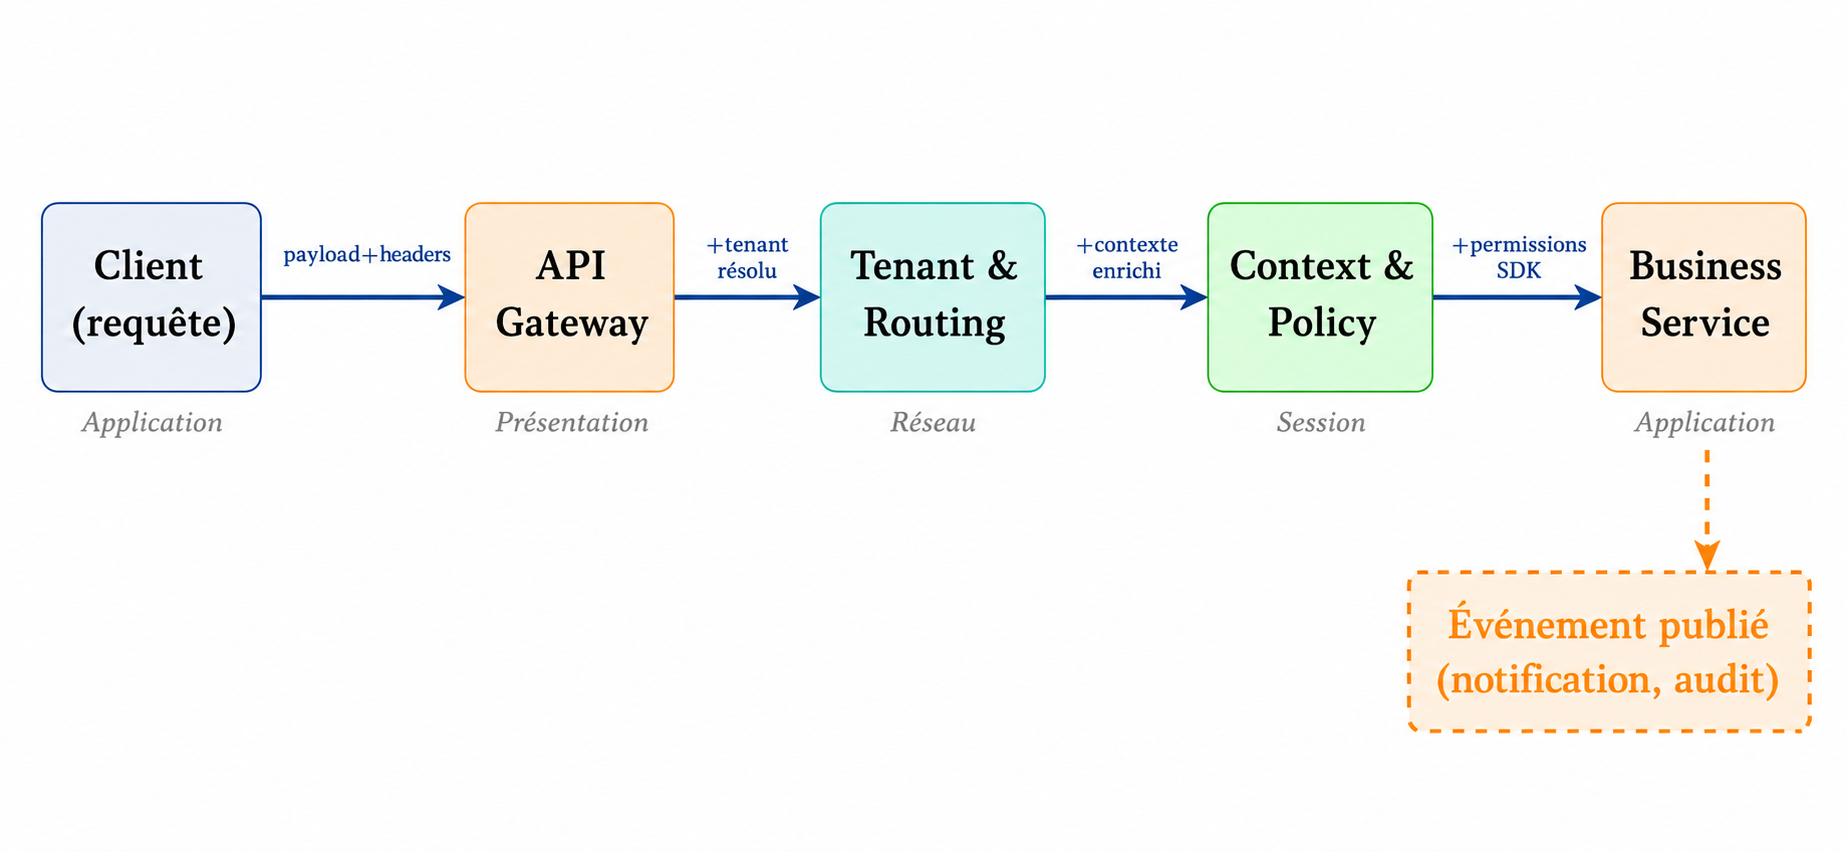
\includegraphics[width=\textwidth]{figures/flux_de_traitement_requete.png}
  \caption{Flux bout-en-bout d'une requête dans BCaaS : Client $\to$ API Gateway $\to$ Tenant \& Routing $\to$ Context \& Policy $\to$ Business Service, avec correspondance OSI descendante/ascendante et publication d'événements (notification, audit).}
  \label{fig:flux}
\end{figure}

\section{La pile protocolaire métier en cinq couches}

De l'analogie découle une décomposition de BCaaS en cinq couches protocolaires, en
correspondance directe avec le modèle OSI (figure~\ref{fig:pile}). Chaque couche n'expose
qu'un service bien défini à la couche supérieure.

\begin{figure}[h]
	\centering
	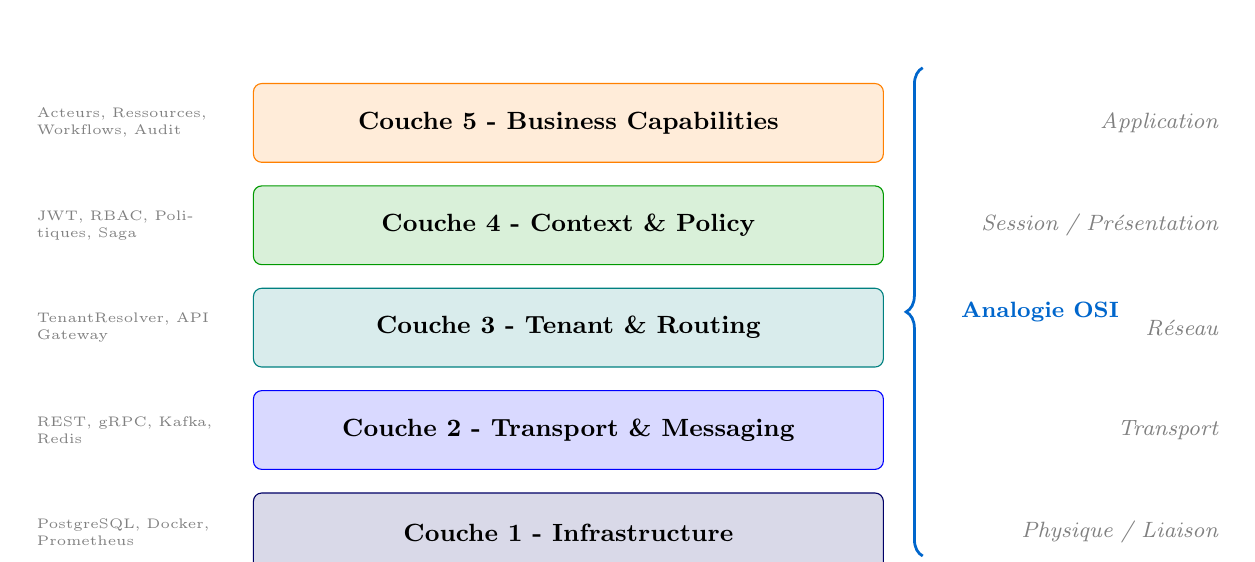
\begin{tikzpicture}[
		layer/.style={draw=#1, fill=#1!15, minimum width=8cm, minimum height=1cm,
			align=center, font=\small\bfseries, rounded corners=3pt},
		rlabel/.style={font=\footnotesize\itshape, text=gray, text width=3.5cm, align=right}
		]
		% Couches
		\node[layer=orange]  (l5) at (0,5.5) {Couche 5 - Business Capabilities};
		\node[layer=green!60!black] (l4) at (0,4.2) {Couche 4 - Context \& Policy};
		\node[layer=teal]    (l3) at (0,2.9) {Couche 3 - Tenant \& Routing};
		\node[layer=blue]    (l2) at (0,1.6) {Couche 2 - Transport \& Messaging};
		\node[layer=blue!40!black] (l1) at (0,0.3) {Couche 1 - Infrastructure};
		
		% Labels droite (analogie OSI)
		\node[rlabel] at (6.5,5.5) {Application};
		\node[rlabel] at (6.5,4.2) {Session / Présentation};
		\node[rlabel] at (6.5,2.9) {Réseau};
		\node[rlabel] at (6.5,1.6) {Transport};
		\node[rlabel] at (6.5,0.3) {Physique / Liaison};
		
		% Labels gauche (technologies)
		\node[font=\tiny, text=gray, align=left, text width=2.5cm] at (-5.5,5.5)
		{Acteurs, Ressources, Workflows, Audit};
		\node[font=\tiny, text=gray, align=left, text width=2.5cm] at (-5.5,4.2)
		{JWT, RBAC, Politiques, Saga};
		\node[font=\tiny, text=gray, align=left, text width=2.5cm] at (-5.5,2.9)
		{TenantResolver, API Gateway};
		\node[font=\tiny, text=gray, align=left, text width=2.5cm] at (-5.5,1.6)
		{REST, gRPC, Kafka, Redis};
		\node[font=\tiny, text=gray, align=left, text width=2.5cm] at (-5.5,0.3)
		{PostgreSQL, Docker, Prometheus};
		
		% Accolades
		\draw[decorate, decoration={brace,amplitude=6pt}, primary, line width=1pt]
		(4.5,0) -- (4.5,6.2) node[midway, right=10pt, font=\footnotesize, primary]
		{\textbf{Analogie OSI}};
	\end{tikzpicture}
	\caption{Pile protocolaire métier de \bcaas{} et correspondance avec le modèle OSI}
	\label{fig:pile}
\end{figure}

\subsection{Couche 1 --- Infrastructure}
Substrat technique : base de données PostgreSQL avec migrations Liquibase, cache Redis et
bus de messages. Elle correspond aux couches physique et liaison : elle transporte les
données sans en connaître la signification.

\subsection{Couche 2 --- Transport \& Messaging}
Analogue à la couche transport (TCP/UDP). Elle gère le mode d'échange (synchrone via REST,
ou asynchrone via le bus d'événements), les stratégies de retry, les timeouts et
l'idempotence. Le choix \emph{REST $\equiv$ TCP} (fiable, ordonné) ou \emph{événement
$\equiv$ UDP} (rapide, au mieux) est explicite dans la conception.

\subsection{Couche 3 --- Tenant \& Routing}
Analogue à la couche réseau. Le \emph{Tenant Resolver} joue le rôle d'un routeur : à partir
de l'en-tête de la requête (le claim \texttt{tenantId} du JWT), il détermine le contexte
d'exécution et oriente la requête vers le bon service. C'est ici que réside la logique de
découverte et d'isolation.

\subsection{Couche 4 --- Context \& Policy}
Analogue aux couches session et présentation. Cette couche valide le token JWT, décode les
rôles et permissions, applique les politiques de sécurité propres au tenant et détermine le
niveau de service. C'est ici qu'est construit l'« en-tête métier » complet de la requête.

\subsection{Couche 5 --- Business Capabilities}
Couche applicative. Elle contient les services métier génériques (acteurs, métiers,
services, ressources, règles, factures, audit), qui opèrent sur des données configurables
par tenant sans connaissance des couches inférieures.

\section{Le multi-tenant comme réseau virtuel (VLAN)}

\begin{analogie}[Analogie : VLAN $\leftrightarrow$ Tenant]
Dans un réseau, un VLAN isole logiquement plusieurs groupes de machines sur la même
infrastructure physique ; chaque trame porte un \emph{tag} (802.1Q) identifiant son
appartenance. Dans BCaaS, chaque requête porte un \texttt{tenant\_id} qui isole les
données, les règles et les workflows d'un client sur l'infrastructure partagée.
\[
\text{tag VLAN} \;\equiv\; \texttt{tenant\_id}, \qquad
\text{réseau physique} \;\equiv\; \text{infrastructure partagée}.
\]
\end{analogie}

\section{Plan de contrôle et plan de données}

\begin{analogie}[Analogie : SDN $\leftrightarrow$ Administration BCaaS]
Dans les réseaux définis par logiciel (SDN), le \emph{control plane} configure de façon
centralisée les règles de routage, tandis que le \emph{data plane} achemine les paquets.
Dans BCaaS, l'interface d'administration (control plane) configure tenants, règles métier,
catalogues et niveaux de service ; le moteur d'exécution (data plane) traite les
transactions en appliquant ces configurations, et émet les événements d'audit et de
notification.

\[
\underbrace{\text{Admin API}}_{\text{Control plane}}
\;\xrightarrow{\text{configuration}}\;
\underbrace{\text{Moteur de transactions}}_{\text{Data plane}}
\;\xrightarrow{\text{exécution}}\;
\underbrace{\text{Audit, Notifications}}_{\text{Événements}}
\]

\end{analogie}
\section{Routage applicatif et recherche de chemin logique}
\label{sec:routage_applicatif}

\begin{analogie}[Analogie : Table de Routage $\leftrightarrow$ Workflow Engine / Handler Resolver]
Dans les infrastructures réseaux, le routage consiste à déterminer le chemin optimal qu'un paquet doit emprunter à travers des nœuds intermédiaires pour atteindre sa destination, en se basant sur des tables de routage dynamiques (alimentées par OSPF ou BGP). 

Dans la plateforme BCaaS, nous transposons ce mécanisme sous la forme d'un \emph{Handler Resolver} couplé à un moteur de règles. Lorsqu'une \texttt{ServiceRequest} franchit les couches de sécurité, le cœur du système inspecte les métadonnées de la requête (le type de service et l'action demandée). À l'instar d'un routeur effectuant un \emph{longest prefix match} sur une adresse IP, le moteur BCaaS effectue une résolution dynamique pour aiguiller le message vers l'instance de composant métier (\emph{Service Handler}) configurée pour ce tenant spécifique.
\end{analogie}

\section{Contrôle de flux et qualité de service (QoS)}
\label{sec:qos_flux}

\begin{analogie}[Analogie : QoS / Token Bucket $\leftrightarrow$ Rate Limiting et SLA]
La mise en commun des ressources physiques au sein d'une infrastructure partagée expose le système au syndrome du \emph{Noisy Neighbor} (un utilisateur saturant les ressources au détriment des autres). En ingénierie des réseaux, ce problème est résolu par des politiques de Qualité de Service (QoS) et des algorithmes de lissage de trafic comme le \emph{Token Bucket}, qui limitent le débit d'un flux à une bande passante allouée.

Au niveau de BCaaS, cette gestion des congestions est implémentée par un mécanisme de \emph{Rate Limiting} adossé aux contrats de niveau de service (\emph{SLA}) des tenants. Chaque requête entrante est soumise à un compteur glissant (géré en cache haute performance via Redis). Si un tenant dépasse le quota de transactions par seconde (TPS) stipulé par ses règles de configuration, le système applique un contrôle de flux strict en rejetant les requêtes excédentaires avec un code statut HTTP 429 (\emph{Too Many Requests}), préservant ainsi la disponibilité globale du \emph{Business Core}.
\end{analogie}



\chapter{Analyse et spécification des besoins}
\label{chap:besoins}

% \section{Acteurs du système}

% Le tableau~\ref{tab:acteurs} décrit les acteurs. Sur le plan métier, une personne physique
% est modélisée par un \texttt{User} rattaché à un tenant ; elle joue un ou plusieurs rôles
% via l'entité \texttt{Actor} (consommateur et/ou fournisseur). Le contrôle d'accès
% applicatif repose sur un ensemble de rôles (\texttt{USER}, \texttt{ADMIN},
% \texttt{PROVIDER}, \texttt{CONSUMER}).

% \begin{table}[H]
% \centering
% \caption{Acteurs du système}
% \label{tab:acteurs}
% \renewcommand{\arraystretch}{1.3}
% \begin{tabularx}{\linewidth}{L{3cm} X L{3.2cm}}
% \toprule
% \textbf{Acteur} & \textbf{Description} & \textbf{Rôles possibles} \\
% \midrule
% Tenant     & Organisation cliente ; contexte d'isolation des données et configurations & --- \\
% User       & Identité authentifiable rattachée à un tenant & USER, ADMIN, PROVIDER, CONSUMER \\
% Consumer (CdS) & Acteur demandeur de services & CONSUMER \\
% Provider (FdS) & Acteur fournisseur de services & PROVIDER \\
% Admin      & Administrateur (plan de contrôle) & ADMIN \\
% \bottomrule
% \end{tabularx}
% \end{table} 
\section{Besoins fonctionnels}

Les besoins fonctionnels sont identifiés par un code \texttt{F-XXX-NNN}. Les
tableaux~\ref{tab:bf-identite} à~\ref{tab:bf-facturation} les regroupent par domaine.

\begin{table}[H]
\centering
\caption{Besoins fonctionnels --- Identités (Tenant, User, Actor)}
\label{tab:bf-identite}
\renewcommand{\arraystretch}{1.25}\footnotesize
\begin{tabularx}{\linewidth}{L{2cm} L{4.6cm} X}
\toprule
\textbf{ID} & \textbf{Fonctionnalité} & \textbf{Contraintes} \\
\midrule
F-TEN-001 & Provisionner un tenant (inscription publique) & Nom et domaine obligatoires, \texttt{tenant\_id} UUID généré \\
F-USR-001 & Inscrire un utilisateur (register) & Email unique, mot de passe chiffré (BCrypt) \\
F-USR-002 & Authentifier (login) & Retourne un JWT portant rôles et \texttt{tenantId} \\
F-USR-003 & Gérer les rôles d'un utilisateur & Réservé au rôle ADMIN \\
F-ACT-001 & Créer un acteur lié à un utilisateur & Un utilisateur peut avoir plusieurs acteurs \\
F-ACT-002 & Filtrer les acteurs par rôle & --- \\
\bottomrule
\end{tabularx}
\end{table}

\begin{table}[H]
\centering
\caption{Besoins fonctionnels --- Métiers (Business, Rule, Catalogue, Resource, Media, Portfolio)}
\label{tab:bf-metier}
\renewcommand{\arraystretch}{1.25}\footnotesize
\begin{tabularx}{\linewidth}{L{2cm} L{4.6cm} X}
\toprule
\textbf{ID} & \textbf{Fonctionnalité} & \textbf{Contraintes} \\
\midrule
F-BUS-001 & Créer / modifier un métier & Nom et domaine obligatoires ; rattaché au tenant \\
F-BUS-002 & Rechercher par domaine & --- \\
F-BRU-001 & Définir une règle métier (clé--valeur) & Rattachée à un Business \\
F-SCA-001 & Créer un service au catalogue & Prix de base + devise validée \\
F-SCA-002 & Filtrer les services disponibles & \texttt{isAvailable} \\
F-RES-001 & Gérer une ressource (stock) & Quantité $\geq 0$ \\
F-MED-001 & Associer un média à un métier & Type + URL \\
F-POR-001 & Gérer un portfolio de compétences & 1 portfolio par acteur ; relation N:M avec Business \\
\bottomrule
\end{tabularx}
\end{table}

\begin{table}[H]
\centering
\caption{Besoins fonctionnels --- Transactions (ServiceRequest, Invoice, Message, Notification)}
\label{tab:bf-facturation}
\renewcommand{\arraystretch}{1.25}\footnotesize
\begin{tabularx}{\linewidth}{L{2cm} L{4.6cm} X}
\toprule
\textbf{ID} & \textbf{Fonctionnalité} & \textbf{Contraintes} \\
\midrule
F-SRE-001 & Créer une demande de service (CdS) & Consumer, provider et service du catalogue requis \\
F-SRE-002 & Faire évoluer le statut & FSM : accept / start / fulfill / cancel \\
F-SRE-003 & Suivre par statut / acteur & --- \\
F-INV-001 & Générer une facture & Automatique à la finalisation (ACK) \\
F-INV-002 & Payer / annuler une facture & FSM : pay / cancel \\
F-MSG-001 & Échanger des messages sur une demande & Temps réel (publication/abonnement) \\
F-NOT-001 & Notifier un utilisateur & Compteur de non-lus, marquage lu \\
F-AUD-001 & Tracer les événements (audit) & Par \texttt{traceId}, acteur, tenant \\
F-ANA-001 & Calculer les KPIs d'un tenant & --- \\
\bottomrule
\end{tabularx}
\end{table}

\section{Besoins non fonctionnels}

Le sujet impose un ensemble exigeant de contraintes non fonctionnelles. Le
tableau~\ref{tab:bnf} en précise le statut dans le présent MVP, dans une logique de
transparence : ce qui n'est pas pleinement réalisé est repris comme perspective au
chapitre~\ref{chap:perspectives}.

\begin{table}[H]
\centering
\caption{Besoins non fonctionnels et statut dans le MVP}
\label{tab:bnf}
\renewcommand{\arraystretch}{1.3}\footnotesize
\begin{tabularx}{\linewidth}{L{3.2cm} X C{2.4cm}}
\toprule
\textbf{Besoin} & \textbf{Description} & \textbf{Statut MVP} \\
\midrule
Multi-tenant & Isolation des données par tenant sur infrastructure partagée & Réalisé \\
Sécurité & Authentification JWT, mots de passe chiffrés, RBAC & Réalisé \\
Multi-devises & Support XAF, XOF, NGN, KES, GHS, USD, EUR, GBP & Réalisé \\
Documentation API & Spécification OpenAPI / Swagger UI & Réalisé \\
Conteneurisation & Docker / docker-compose & Réalisé \\
Modularité (DDD / hexagonal) & Monolithe modulaire, microservices-ready & Réalisé \\
Temps réel & Messagerie instantanée sur les demandes & Partiel (Redis pub/sub) \\
Événementiel & Bus d'événements (notifications, audit) & Partiel (infra posée) \\
Géo-référencement & PostGIS, géolocalisation native & Perspective \\
Offline-first / PWA & Application installable et hors-ligne & Perspective \\
Internationalisation & i18n web et mobile & Perspective \\
Réactif & WebFlux + R2DBC non bloquant & Perspective \\
2FA & Double authentification & Perspective \\
Mobile natif & React Native & Perspective \\
\bottomrule
\end{tabularx}
\end{table}

\section{Diagramme de contexte}
\begin{figure}[H]
    \centering
    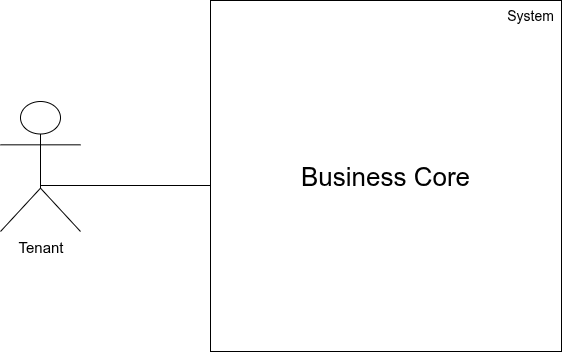
\includegraphics[width=0.8\linewidth]{chapitres/diagramme de contexte.drawio.png }
    \captionof{figure}{Diagramme de contexte du système}
    \label{fig:placeholder}
\end{figure}

\chapter{Modélisation mathématique}
\label{chap:math}

Ce chapitre propose une formalisation ensembliste du système, de ses contraintes et de ses
indicateurs. Cette modélisation explicite les invariants que l'implémentation doit garantir
et fournit un langage rigoureux pour raisonner sur le matching et les performances.

\section{Ensembles fondamentaux}

Le système est décrit par les ensembles d'entités suivants, tous identifiés par des UUID :
\[
\begin{aligned}
&T \text{ (Tenants)}, \quad U \text{ (Users)}, \quad A \text{ (Actors)}, \quad
B \text{ (Businesses)}, \quad S \text{ (ServiceCatalogues)}, \\
&R \text{ (Resources)}, \quad Po \text{ (Portfolios)}, \quad SR \text{ (ServiceRequests)},
\quad I \text{ (Invoices)}, \quad BR \text{ (BusinessRules)}.
\end{aligned}
\]
L'ensemble des devises supportées est fini :
\[
C = \{\text{XAF, XOF, NGN, KES, GHS, USD, EUR, GBP}\}.
\]

\subsection{Décomposition des acteurs}
\[
A = A_{c} \cup A_{p}, \qquad A_{c} \cap A_{p} \neq \emptyset,
\]
où $A_c$ (consommateurs) et $A_p$ (fournisseurs) peuvent se recouper : un même acteur peut
à la fois consommer et fournir des services.

\subsection{Attributs des entités principales}
\begin{align*}
t  &= (\mathit{id}_T, \text{name}, \text{domain}, \text{isActive}, \text{createdAt}) \in T,\\
u  &= (\mathit{id}_U, \text{tenant}, \text{email}, \text{roles}, \text{isActive}, \dots) \in U,\\
a  &= (\mathit{id}_A, \text{user}, \text{role}, \text{bio}, \text{isActive}) \in A,\\
sr &= (\mathit{id}_{SR}, \text{tenant}, \text{consumer}, \text{provider}, \text{catalogue},
       \text{status}, \text{traceId}, \dots) \in SR,\\
i  &= (\mathit{id}_I, \text{serviceRequest}, \text{amount}, \text{currency}, \text{status},
       \text{issuedAt}, \text{paidAt}) \in I.
\end{align*}

\section{Variables de décision et fonction objectif}

\subsection{Variables}
Variable binaire de matching :
\[
x_{a_c, a_p, b} \in \{0,1\}, \quad \forall (a_c, a_p, b) \in A_c \times A_p \times B,
\]
valant $1$ si le consommateur $a_c$ est mis en relation avec le fournisseur $a_p$ pour le
métier $b$. Variable d'état d'une demande :
\[
\sigma_{sr} \in \Sigma_{SR} = \{\text{PENDING, ACCEPTED, IN\_PROGRESS, FULFILLED, CANCELLED}\}.
\]
\iffalse
\subsection{Objectif multi-critère}
On cherche à maximiser le nombre de transactions réussies et le chiffre d'affaires, tout en
minimisant la durée de traitement :
\[
\max\; \alpha \sum_{sr \in SR} \mathbb{1}_{\sigma_{sr} = \text{FULFILLED}}
     + \beta  \sum_{i \in I} \text{amount}(i)\,\mathbb{1}_{\sigma_i = \text{PAID}}
     - \gamma \sum_{sr \in SR} \text{duration}(sr),
\]
\[
\text{avec } \alpha + \beta + \gamma = 1, \quad \alpha,\beta,\gamma \geq 0.
\]
\fi

\section{Contraintes du système}

\subsection{Contraintes de cardinalité}
\begin{align}
&\forall u_1, u_2 \in U,\ u_1 \neq u_2 : \ u_1.\text{email} \neq u_2.\text{email}
   &&\text{(unicité de l'email)}\\
&\forall a \in A,\ \exists!\, po \in Po : po.\text{actor} = a
   &&\text{(Actor} \to \text{Portfolio, 1:1)}\\
&\forall po \in Po : \ po.\text{businesses} \subseteq B
   &&\text{(Portfolio} \to \text{Business, N:M)}\\
&\forall sr \in SR,\ \exists!\, i \in I : i.\text{serviceRequest} = sr
   &&\text{(ServiceRequest} \to \text{Invoice, 1:1)}
\end{align}

\subsection{Contraintes métier}
Validité d'une demande :
\[
\text{valid}(sr) \iff
\begin{cases}
sr.\text{consumer}.\text{role} = \text{CONSUMER},\\
sr.\text{provider}.\text{role} = \text{PROVIDER},\\
sr.\text{provider}.\text{isActive} = \text{vrai}.
\end{cases}
\]
Compatibilité de matching :
\[
\text{compatible}(a_c, a_p, b) \iff \exists\, po \in Po :
\big(po.\text{actor} = a_p \ \wedge\ b \in po.\text{businesses}\big).
\]
Contrainte de devise :
\[
\forall i \in I : i.\text{currency} \in C, \qquad \forall s \in S : s.\text{currency} \in C.
\]
Contrainte d'isolation multi-tenant (invariant de sécurité) :
\[
\forall sr \in SR : sr.\text{tenant} = \tau \implies
\big(sr.\text{consumer}.\text{user}.\text{tenant} = \tau \ \wedge\
      sr.\text{catalogue}.\text{business}.\text{tenant} = \tau\big).
\]

\subsection{Contrainte de workflow : machine à états}
Soit $\delta_{SR} : \Sigma_{SR} \times \mathcal{A} \to \Sigma_{SR}$ la fonction de
transition, avec $\mathcal{A} = \{\text{create, accept, start, fulfill, cancel}\}$. Les
transitions valides sont données au tableau~\ref{tab:fsm-math}.

\begin{table}[H]
\centering
\caption{Transitions valides de la machine à états \texttt{ServiceRequest}}
\label{tab:fsm-math}
\renewcommand{\arraystretch}{1.2}\footnotesize
\begin{tabular}{lll}
\toprule
\textbf{État courant} & \textbf{Action} & \textbf{État suivant} \\
\midrule
$\emptyset$    & create  & PENDING \\
PENDING        & accept  & ACCEPTED \\
PENDING        & cancel  & CANCELLED \\
ACCEPTED       & start   & IN\_PROGRESS \\
ACCEPTED       & cancel  & CANCELLED \\
IN\_PROGRESS   & fulfill & FULFILLED \\
IN\_PROGRESS   & cancel  & CANCELLED \\
\bottomrule
\end{tabular}
\end{table}

\section{Algorithmes et complexité}

\subsection{Recherche des fournisseurs d'un métier}
\begin{lstlisting}[language={},caption={FindProvidersByBusiness},captionpos=b]
Entree : b (business cible)
Sortie : ensemble des providers compatibles
1: Resultat <- vide
2: pour chaque po dans Po :
3:     si b appartient a po.businesses :
4:         a <- po.actor
5:         si a.role = PROVIDER et a.isActive : Resultat <- Resultat U {a}
6: retourner Resultat
\end{lstlisting}
\textbf{Complexité :} $O(|Po|)$ dans le pire cas, $O(1)$ amorti avec un index sur les
métiers du portfolio.

\subsection{Recherche par filtres combinés}
Pour un ensemble de filtres $F = \{f_1, \dots, f_n\}$, le résultat est l'intersection
\[
\text{result}(F) = \bigcap_{f \in F} \text{applyFilter}(f, \text{Univers}),
\]
optimisée en appliquant d'abord le filtre le plus sélectif :
\[
\text{selectivity}(f) = \frac{|\text{applyFilter}(f, \text{Univers})|}{|\text{Univers}|},
\qquad \text{ordre croissant de } \text{selectivity}.
\]

\section{Indicateurs et métriques (KPIs)}

Sur une période $[t_1, t_2]$, on définit :
\[
\boxed{T_{\text{conv}} = \frac{N_{\text{fulfilled}}}{N_{\text{requests}}} \times 100\%},
\qquad
\boxed{PA = \frac{CA}{N_{\text{paid}}}},
\]
où le chiffre d'affaires est
\[
CA(t_1, t_2) = \sum_{\substack{i \in I \,:\, \sigma_i = \text{PAID}\\ i.\text{paidAt} \in [t_1,t_2]}}
i.\text{amount},
\]
et le temps moyen de réalisation
\[
\boxed{T_{\text{compl}} = \frac{1}{N_{\text{fulfilled}}}
\sum_{\substack{sr \in SR \,:\, \sigma_{sr} = \text{FULFILLED}}}
\big(sr.\text{fulfilledAt} - sr.\text{requestedAt}\big)}.
\]
La part d'un métier $b$ dans le chiffre d'affaires s'écrit
$\text{Share}_b = CA_b / CA \times 100\%$, et la croissance mensuelle
$\text{Growth}_{\text{MoM}}(t) = (CA(t) - CA(t-1)) / CA(t-1) \times 100\%$. Ces indicateurs
sont calculés par le service d'analytique 
% ════════════════════════════════════════════════════════
% À COLLER DIRECTEMENT APRÈS LA DERNIÈRE LIGNE DU 5.5
% Aucun package ou couleur supplémentaire requis.
% ════════════════════════════════════════════════════════

\section{Architecture en couches : composition de fonctions}

Ce modèle formalise le traitement d'une requête à travers les cinq
couches de BCaaS. Chaque couche est représentée par une fonction de
transformation, et le traitement complet est leur composée.

\subsection{Définition formelle}

On associe à chaque couche $i \in \{1,\ldots,5\}$ une fonction :
\begin{align*}
f_1 &: r   \mapsto r_1 && \text{Infrastructure (connexion BD, cache)}\\
f_2 &: r_1 \mapsto r_2 && \text{Transport \& Messaging (REST ou Kafka)}\\
f_3 &: r_2 \mapsto r_3 && \text{Tenant \& Routing (résolution \texttt{tenant\_id})}\\
f_4 &: r_3 \mapsto r_4 && \text{Context \& Policy (JWT, RBAC, SLA)}\\
f_5 &: r_4 \mapsto r_5 && \text{Business Capabilities (logique métier)}
\end{align*}

Le traitement complet d'une requête $r$ est la \textbf{composée} de
ces cinq fonctions :
\[
\text{BCaaS}(r)
\;=\;
(f_5 \circ f_4 \circ f_3 \circ f_2 \circ f_1)(r)
\;=\;
f_5\!\Bigl(f_4\!\bigl(f_3\!\bigl(f_2\!\bigl(f_1(r)\bigr)\bigr)\bigr)\Bigr).
\]

\subsection{Propriété : encapsulation stricte}

Pour tout $i \in \{1,\ldots,5\}$, la fonction $f_i$ ne reçoit en entrée
que $r_{i-1}$ et est indépendante de $f_j$ pour tout $j > i$ :
\[
f_i \;:\; \mathcal{R}_{i-1} \;\longrightarrow\; \mathcal{R}_i,
\qquad f_i \perp f_j \text{ pour } j > i.
\]
Modifier $f_5$ n'affecte jamais $f_1$ : c'est la traduction formelle du
principe d'encapsulation du modèle OSI.

\subsection{Exemple}

Considérons une \texttt{ServiceRequest} de création de métier
(\texttt{POST /api/businesses}) émise par un acteur authentifié.
La requête $r$ traverse les cinq couches :
$f_1$ ouvre la connexion PostgreSQL,
$f_2$ sélectionne le transport REST synchrone,
$f_3$ résout le \texttt{tenant\_id} depuis l'en-tête \texttt{X-Tenant-ID},
$f_4$ valide le token JWT et le rôle \texttt{ADMIN},
et $f_5$ persiste l'entité et retourne \texttt{201 Created} :
\[
\text{BCaaS}(r) = f_5\bigl(f_4\bigl(f_3\bigl(f_2\bigl(f_1(r)\bigr)\bigr)\bigr)\bigr)
= r_5 = \texttt{201 Created}.
\]
Si $f_4$ échoue (JWT expiré), la composition s'arrête en $r_4$ et
retourne \texttt{401 Unauthorized}, sans jamais atteindre $f_5$.


\section{Isolation multi-tenant : théorie des ensembles}

Ce modèle formalise l'étanchéité des données entre les tenants de
l'ensemble $T$ (défini à la section~5.1). Il constitue la preuve
ensembliste globale de la contrainte d'isolation posée à la section~5.3.

\subsection{Définitions}

On note $\mathcal{E}$ l'ensemble de toutes les lignes présentes en base
de données (tables $U$, $A$, $B$, $SR$, $I$, etc. confondues).
On définit la fonction d'appartenance $\pi : \mathcal{E} \to T$ par :
\[
\pi(e) = \tau_k
\quad \Longleftrightarrow \quad
\text{la colonne \texttt{tenant\_id} de } e \text{ vaut } \tau_k.
\]
L'ensemble des données du tenant $\tau_k$ est :
\[
\mathcal{D}(\tau_k) \;=\; \bigl\{\, e \in \mathcal{E} \;\big|\; \pi(e) = \tau_k \,\bigr\}.
\]

\subsection{Propriété : isolation totale}

\[
\forall\, \tau_i, \tau_j \in T,\quad
\tau_i \neq \tau_j
\;\implies\;
\mathcal{D}(\tau_i) \cap \mathcal{D}(\tau_j) = \emptyset.
\]

Les ensembles $\mathcal{D}(\tau_1), \ldots, \mathcal{D}(\tau_n)$
forment une \textbf{partition} de $\mathcal{E}$ :
\[
\mathcal{E}
\;=\;
\biguplus_{k=1}^{n} \mathcal{D}(\tau_k)
\;=\;
\mathcal{D}(\tau_1) \;\uplus\; \mathcal{D}(\tau_2)
\;\uplus\; \cdots \;\uplus\; \mathcal{D}(\tau_n).
\]
Aucune entité n'est « sans tenant » ni « dans deux tenants à la fois ».
Cette propriété est garantie dans le code par le \texttt{TenantFilter}
de Spring Security, qui injecte le \texttt{tenant\_id} dans chaque
requête SQL via un \texttt{ThreadLocal}.

\subsection{Exemple}

Deux tenants sont inscrits : $\tau_1$ (Auto-École Centrale) et
$\tau_2$ (Clinique Mélen). Les \texttt{ServiceRequests} associées sont :
\[
\mathcal{D}(\tau_1) = \{sr_1, sr_2, sr_3\},
\qquad
\mathcal{D}(\tau_2) = \{sr_4, sr_5\},
\qquad
\mathcal{D}(\tau_1) \cap \mathcal{D}(\tau_2) = \emptyset.
\]
Un acteur de $\tau_2$ exécutant \texttt{GET /api/service-requests} ne
verra jamais $sr_1$, $sr_2$ ou $sr_3$ : le \texttt{TenantFilter} ajoute
automatiquement \texttt{WHERE tenant\_id = '$\tau_2$'} à chaque requête.


\section{Provisionnement d'un tenant : suite finie d'états}

Ce modèle formalise l'inscription d'un nouveau tenant comme une suite
d'états atomiques. Il est distinct de la machine à états des
\texttt{ServiceRequests} (section~5.3.3) : il ne s'exécute qu'une seule
fois par tenant, au moment de son inscription sur la plateforme.

\subsection{Les sept états du provisionnement}

Soit $\mathcal{S} = (S_0, S_1, \ldots, S_6)$ la suite des états :

\begin{table}[H]
\centering
\caption{Suite d'états du provisionnement d'un tenant}
\label{tab:prov-states}
\renewcommand{\arraystretch}{1.2}\small
\begin{tabular}{lll}
\toprule
\textbf{État} & \textbf{Nom} & \textbf{Description et précondition} \\
\midrule
$S_0$ & Requête reçue
  & Réception de \texttt{POST /api/tenants \{name, domain, sla\}}. \\
$S_1$ & Validation du domaine
  & \textbf{Précondition :}
    $\text{dom}_{\text{req}} \notin \{t.\text{domain} \mid t \in T\}$.
    Sinon : \texttt{409 Conflict}. \\
$S_2$ & Génération de l'id
  & Génération d'un $\text{id} \in \text{UUID}_4$
    (collision $\approx 10^{-36}$). \\
$S_3$ & Insertion en base
  & \texttt{INSERT INTO tenant} en transaction atomique.
    Rollback si échec. \\
$S_4$ & Contexte d'isolation
  & Initialisation $\mathcal{D}(t_{\text{new}}) \leftarrow \emptyset$,
    \texttt{TenantFilter} configuré. \\
$S_5$ & Génération JWT
  & Token signé $(\text{tenant\_id}, \text{roles}, \exp)$,
    $\exp = t_{\text{now}} + 24\,\text{h}$. \\
$S_6$ & Tenant actif
  & $t_{\text{new}} \in T$ et
    $\mathcal{D}(t_{\text{new}}) = \emptyset$. \\
\bottomrule
\end{tabular}
\end{table}

\subsection{Propriété : injectivité du domaine}

La précondition de $S_1$ garantit que la fonction
$\text{domain} : T \to \mathit{Dom}$ est \textbf{injective} :
\[
\text{domain}(t_i) = \text{domain}(t_j) \;\implies\; t_i = t_j.
\]
Deux tenants distincts ne peuvent jamais partager le même domaine.
Cette propriété complète les contraintes de cardinalité de la
section~5.3 et est analogue à l'unicité des adresses IP sur un
réseau : elle permet un routage sans ambiguïté par $f_3$ (section~5.6).

\subsection{Exemple}

Un gestionnaire soumet
\texttt{POST /api/tenants \{"domain":"cabinet-dupont"\}}.
En $S_1$, le système vérifie
$\texttt{"cabinet-dupont"} \notin \{t.\text{domain} \mid t \in T\}$ :
précondition satisfaite.
En $S_2$, l'UUID \texttt{b9c2-4f1a-\ldots} est généré.
En $S_3$, la ligne est insérée de façon atomique.
En $S_4$, $\mathcal{D}(t_{\text{new}}) \leftarrow \emptyset$.
En $S_5$, le JWT initial est signé.
En $S_6$ :
\[
t_{\text{new}} \in T, \quad
\mathcal{D}(t_{\text{new}}) = \emptyset, \quad
\text{domain}(t_{\text{new}}) = \texttt{"cabinet-dupont"}.
\]
Si une seconde requête tentait le même domaine, $S_1$ retournerait
\texttt{409 Conflict}, préservant l'injectivité.
(chapitre~\ref{chap:observ}).

\chapter{Conception architecturale}
\label{chap:archi}

La pile protocolaire en cinq couches qui structure la lecture de BCaaS a été présentée au
chapitre~\ref{chap:analogie} (figure~\ref{fig:pile}). Le présent chapitre se concentre sur
les choix d'architecture logicielle qui la concrétisent : l'architecture hexagonale, le
monolithe modulaire et l'organisation en packages.

\section{Architecture hexagonale et DDD}

BCaaS adopte une architecture hexagonale (ports et adaptateurs) combinée au Domain-Driven
Design. Le domaine métier (entités, règles, machines à états) est isolé au centre ;
les détails techniques (persistance JPA, exposition REST, messagerie) sont relégués aux
adaptateurs périphériques. Cette organisation garantit que le cœur métier ne dépend
d'aucune technologie particulière, condition d'une évolution ultérieure sereine.

Concrètement, le flux d'une requête traverse les couches applicatives suivantes :
\[
\text{Controller (REST)} \to \text{Service (domaine)} \to \text{Repository (JPA)} \to
\text{Base de données},
\]
les DTO assurant le découplage entre la représentation exposée et les entités persistées.

\section{Monolithe modulaire « microservices-ready »}

Conformément aux contraintes du sujet, BCaaS est un \textbf{monolithe modulaire} : les
modules métier (acteurs, métiers, catalogues, demandes, factures, audit, analytique) sont
organisés en packages cohérents et communiquent par appels en mémoire. Ce choix simplifie
le déploiement et la coordination initiale tout en préservant des frontières nettes : les
modules pourront, à terme, être extraits en microservices déployés indépendamment, sans
réécrire le domaine (perspective détaillée au chapitre~\ref{chap:perspectives}).

%\figplaceholder{Architecture logique de BCaaS : API %Gateway (Auth JWT, routing,
%%X-Tenant-ID) au-dessus des modules métier (Actor, %Business, Service Catalogue, Service
%Request, Invoice, Resource, Media, Notification, %Audit, Analytics), reposant sur
%l'infrastructure (PostgreSQL, Redis, bus %d'événements).}{6.5cm}

\begin{figure}[H]
    \centering
    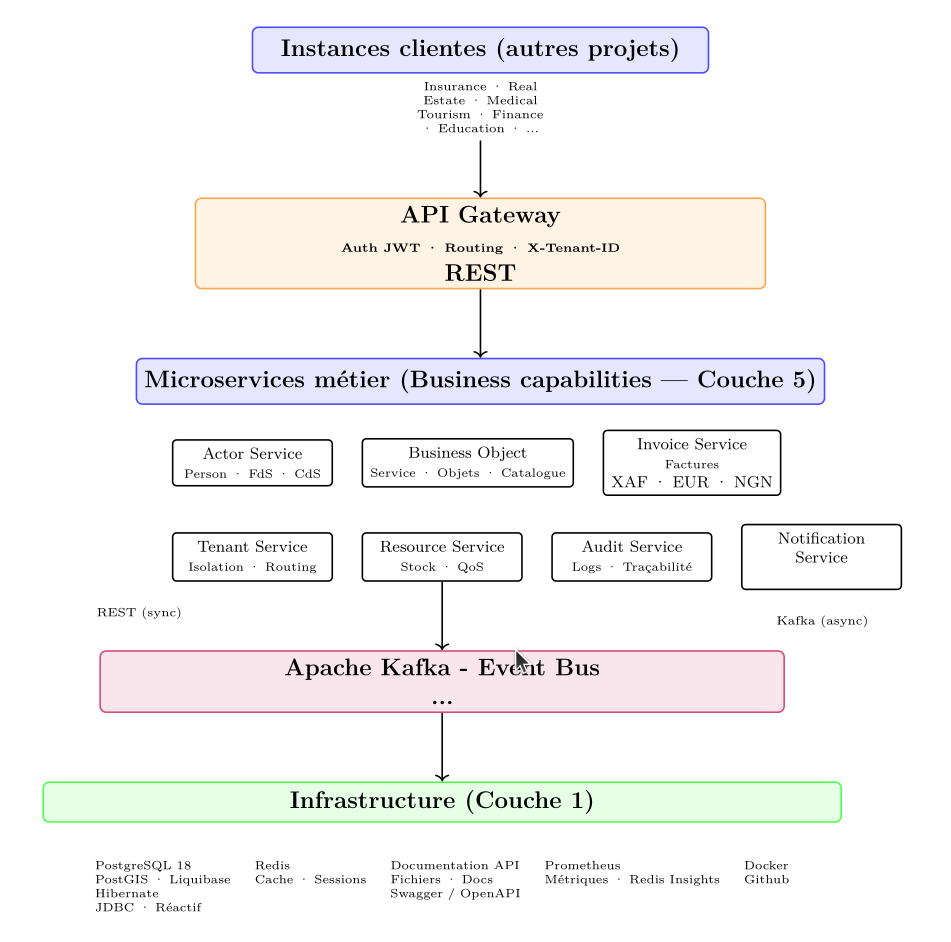
\includegraphics[width=0.8\linewidth]{chapitres/Capture d’écran du 2026-06-16 08-18-23.png}
    \captionof{figure}{Architecture logique de BCaaS}
    \label{fig:placeholder}
\end{figure}


\section{Diagramme de packages}

L'organisation en packages reflète les domaines fonctionnels : authentification, gestion
des acteurs, gestion des métiers, gestion des services, gestion des médias, gestion des
ressources et gestion des factures. Chaque package porte des responsabilités bien
délimitées, ce qui facilite l'évolution indépendante des règles métier et des mécanismes

\paragraph{Tenant}
L'acteur Tenant suggère une architecture multi-tenant, où chaque client (organisation ou locataire) dispose de sa propre isolation des données et configurations. Ce package agit probablement comme un contexte global d'exécution permettant aux autres modules de fonctionner de manière isolée par tenant.

\paragraph{Authentification et gestion des acteurs}
Le package AUTHENTIFICATION gère les processus d'identification et de vérification des tenants. Il interagit directement avec GESTION DES ACTEURS qui centralise la définition, les rôles et les permissions des différentes entités utilisatrices (administrateurs, clients, fournisseurs, etc.). Cette séparation permet de dissocier le mécanisme technique d'authentification de la gestion administrative des profils.

\paragraph{Gestion des business et services}
Les packages GESTION DES BUSINESS et GESTION DES SERVICES couvrent le cœur métier. Le premier traite des règles propres à l'activité de l'entreprise, tandis que le second coordonne l'information, l'orchestration ou la souscription aux services proposés. Leur découpage facilite l'évolution indépendante des règles métier et des mécanismes de service.

\paragraph{Gestion des médias, ressources et factures}
Le package GESTION DES MEDIA est dédié aux contenus multimédias (images, vidéos, documents). GESTION DES RESSOURCES supervise les actifs techniques ou matériels nécessaires au fonctionnement (serveurs, licences, matériel, équipements). Enfin, GESTION DES FACTURES assure la chaîne de facturation, de la génération des factures au suivi des paiements.

%\figplaceholder{Diagramme de packages UML : %AUTHENTIFICATION, GESTION DES ACTEURS, GESTION
%DES BUSINESS, GESTION DES SERVICES, GESTION DES MEDIA, %GESTION DES RESSOURCES, GESTION DES
%FACTURES, sous le contexte multi-tenant.}{6.5cm}

\begin{figure}[H]
    \centering
    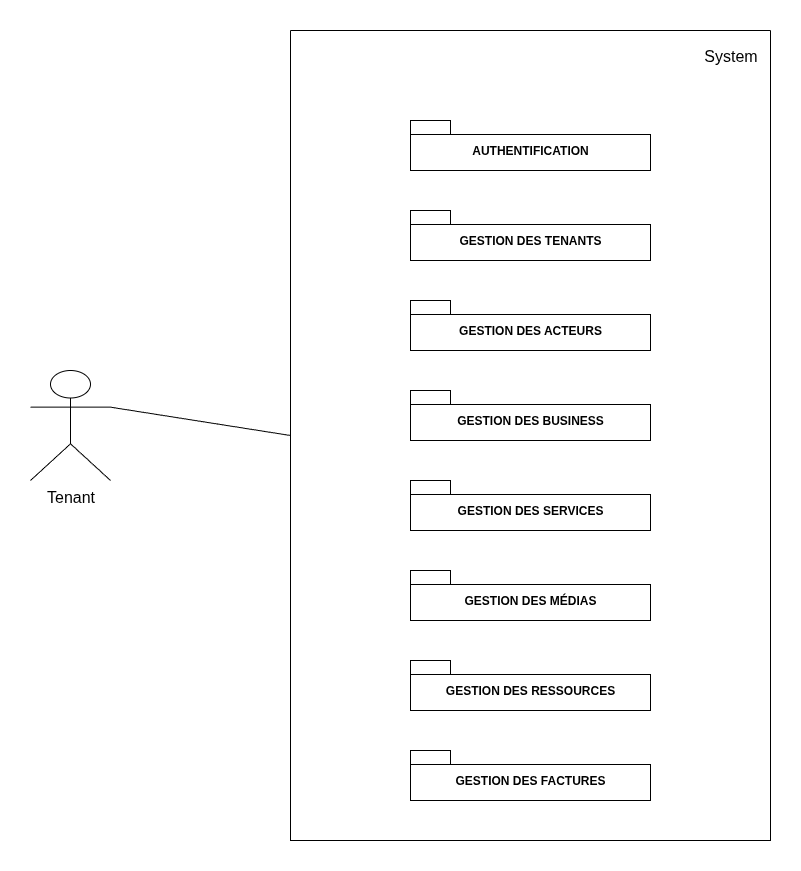
\includegraphics[width=0.8\linewidth]{chapitres/package.drawio.png}
   \captionof{figure}{Diagramme de packages de l'architecture du système}
    \label{fig:placeholder}
\end{figure}
\label{fig:packages}


\chapter{Conception détaillée des données}
\label{chap:donnees}

Le défi central de BCaaS est de modéliser des entités métier hétérogènes (médecin, livre,
appartement, produit agricole, etc.) avec un schéma de données unique et générique. Nous
adoptons une modélisation Merise (MCD, MLD) complétée par un diagramme de classes UML.

%\section{Modèle Conceptuel de Données (MCD)}

%\figplaceholder{Modèle Conceptuel de Données (Merise) %: entités TENANT, USER, ACTOR,
%PORTFOLIO, BUSINESS, BUSINESS\_RULE, %SERVICE\_CATALOGUE, RESOURCE, MEDIA, SERVICE\_REQUEST,
%INVOICE, MESSAGE, NOTIFICATION, AUDIT\_EVENT et leurs %associations avec cardinalités.}{7.5cm}
%\captionof{figure}{Modèle Conceptuel de Données de %BCaaS}
%\label{fig:mcd}

\section{Dictionnaire des entités}

Le domaine compte quinze entités (plus l'énumération \texttt{SupportedCurrency} et la table
de jonction \texttt{portfolio\_businesses}). Le tableau~\ref{tab:entites} en récapitule la
structure.

\begin{table}[H]
\centering
\caption{Entités du modèle de données --- Business Core}
\label{tab:entites}
\renewcommand{\arraystretch}{1.25}\scriptsize
\begin{tabularx}{\linewidth}{L{2.5cm} X}
\toprule
\textbf{Entité (table)} & \textbf{Attributs principaux et relations} \\
\midrule
\texttt{Tenant} (tenants) & \texttt{id}, \texttt{name} (unique), \texttt{domain}, \texttt{description}, \texttt{isActive}, \texttt{createdAt}. Racine du multi-tenant. \\
\texttt{User} (users) & \texttt{id}, \texttt{firstName}, \texttt{lastName}, \texttt{email} (unique), \texttt{password}, \texttt{phone}, \texttt{country}, \texttt{roles} (Set), \texttt{isActive}, \texttt{createdAt} ; \texttt{ManyToOne} $\to$ Tenant. \\
\texttt{Actor} (actors) & \texttt{id}, \texttt{role}, \texttt{bio}, \texttt{isActive}, \texttt{createdAt} ; \texttt{ManyToOne} $\to$ User. \\
\texttt{Business} (businesses) & \texttt{id}, \texttt{name}, \texttt{domain}, \texttt{description}, \texttt{typeOfInvolvedActors}, \texttt{requiredJobProfile}, \texttt{createdAt} ; \texttt{ManyToOne} $\to$ Tenant. \\
\texttt{BusinessRule} (business\_rules) & \texttt{id}, \texttt{ruleKey}, \texttt{ruleValue}, \texttt{description}, \texttt{createdAt} ; \texttt{ManyToOne} $\to$ Business. \\
\texttt{ServiceCatalogue} (service\_catalogues) & \texttt{id}, \texttt{name}, \texttt{description}, \texttt{basePrice}, \texttt{currency}, \texttt{isAvailable}, \texttt{createdAt} ; \texttt{ManyToOne} $\to$ Business. \\
\texttt{Resource} (resources) & \texttt{id}, \texttt{name}, \texttt{type}, \texttt{quantity}, \texttt{description}, \texttt{createdAt} ; \texttt{ManyToOne} $\to$ Business. \\
\texttt{Media} (media) & \texttt{id}, \texttt{type}, \texttt{url}, \texttt{label}, \texttt{createdAt} ; \texttt{ManyToOne} $\to$ Business. \\
\texttt{Portfolio} (portfolios) & \texttt{id}, \texttt{title}, \texttt{description}, \texttt{createdAt} ; \texttt{OneToOne} $\to$ Actor ; \texttt{ManyToMany} $\to$ Business (\texttt{portfolio\_businesses}). \\
\texttt{ServiceRequest} (service\_requests) & \texttt{id}, \texttt{serviceName}, \texttt{description}, \texttt{status}, \texttt{traceId}, \texttt{correlationId}, 5 timestamps ; \texttt{ManyToOne} $\to$ Tenant, consumer Actor, provider Actor, ServiceCatalogue. \\
\texttt{Invoice} (invoices) & \texttt{id}, \texttt{amount}, \texttt{currency}, \texttt{status}, \texttt{issuedAt}, \texttt{paidAt} ; \texttt{OneToOne} $\to$ ServiceRequest (unique). \\
\texttt{Message} (messages) & \texttt{id}, \texttt{content}, \texttt{isRead}, \texttt{createdAt} ; \texttt{ManyToOne} $\to$ ServiceRequest, sender Actor, Tenant. \\
\texttt{Notification} (notifications) & \texttt{id}, \texttt{title}, \texttt{message}, \texttt{isRead}, \texttt{createdAt} ; \texttt{ManyToOne} $\to$ User, Tenant. \\
\texttt{AuditEvent} (audit\_events) & \texttt{id}, \texttt{entityType}, \texttt{action}, \texttt{previousStatus}, \texttt{newStatus}, \texttt{ipAddress}, \texttt{userAgent}, \texttt{metadata} (JSON), \texttt{tenantId}, \texttt{actorId}, \texttt{entityId}, \texttt{traceId} (UUID bruts). \\
\bottomrule
\end{tabularx}
\end{table}

\noindent Toutes les entités utilisent une génération d'identifiant
\texttt{GenerationType.UUID} et un \texttt{@PrePersist} initialisant \texttt{createdAt}.

\section{Modèle Logique de Données (MLD)}

Le passage au modèle relationnel traduit les associations par des clés étrangères. En
particulier, l'isolation multi-tenant repose sur une colonne \texttt{tenant\_id} (UUID,
clé étrangère vers \texttt{tenants}) portée par les tables racines du tenant
(\texttt{users}, \texttt{businesses}, \texttt{service\_requests}, \texttt{messages},
\texttt{notifications}, \texttt{audit\_events}). L'entité \texttt{Actor} n'a pas de
\texttt{tenant\_id} direct : elle hérite du contexte tenant via son \texttt{User}.

%\figplaceholder{Modèle Logique de Données (schéma %relationnel) : tables et clés étrangères,
%mise en évidence des colonnes \texttt{tenant\_id} et %des contraintes d'unicité.}{6.5cm}
%\captionof{figure}{Modèle Logique de Données de BCaaS}
%\label{fig:mld}

\begin{table}[h]
\centering
\caption{Entités du modèle de données – Business Core}
\label{tab:entites_business_core}
\begin{tabular}{|p{4cm}|p{12cm}|}
\hline
\textbf{Table} & \textbf{Attributes} \\
\hline
tenant & id\_Tenant, Name, IsActive, CreatedAt \\
\hline
user & Id\_User, FirstName, LastName, Email, Gender, Password, IsActive, Country, Phone, CreatedAt, \#id\_Tenant \\
\hline
actor & Id\_Actor, NomProfessionnel, Speciality, bio, CreatedAt, Role, \#Id\_User \\
\hline
formation & Id\_Formation, NomFormation, Description, Type\_Formation, Niveau \\
\hline
media & Id\_Media, Type, Url, Label, CreatedAt, \#Id\_Business \\
\hline
business & Id\_Business, NameBusiness, Domain, Type\_of\_InvolvedActors, RequiredJobProfile, CreatedAt \\
\hline
business\_rule & Id\_BusinessRule, RuleKey, RuleValue, Description, CreatedAt \\
\hline
ressource & Id\_Resource, NameRes, Type, Quantity, Description, CreatedAt, Disponibilité \\
\hline
service\_catalogue & Id\_SerCatalogue, NameSerCatalogue, Description, Currency, IsAvailable, CreatedAt \\
\hline
portfolio & Id\_Portfolio, title, Description, Status, \#Id\_Business \\
\hline
service\_request & Id\_ServiceRequest, TraceId, ServiceName, Description, Status, \#Id\_Actor, \#Id\_Portfolio \\
\hline
message & id\_Message, content, isRead, createdAt, \#Id\_ServiceRequest \\
\hline
notification & id\_Notification, title, message, isRead, createdAt, \#Id\_ServiceRequest \\
\hline
invoice & id\_Invoice, Amount, Currency, Status, UsedAt, PaidAt, IssueAt, \#Id\_ServiceRequest \\
\hline
\end{tabular}
\end{table}

\section{Diagramme de classes métier}

\begin{figure}[H]
    \centering
    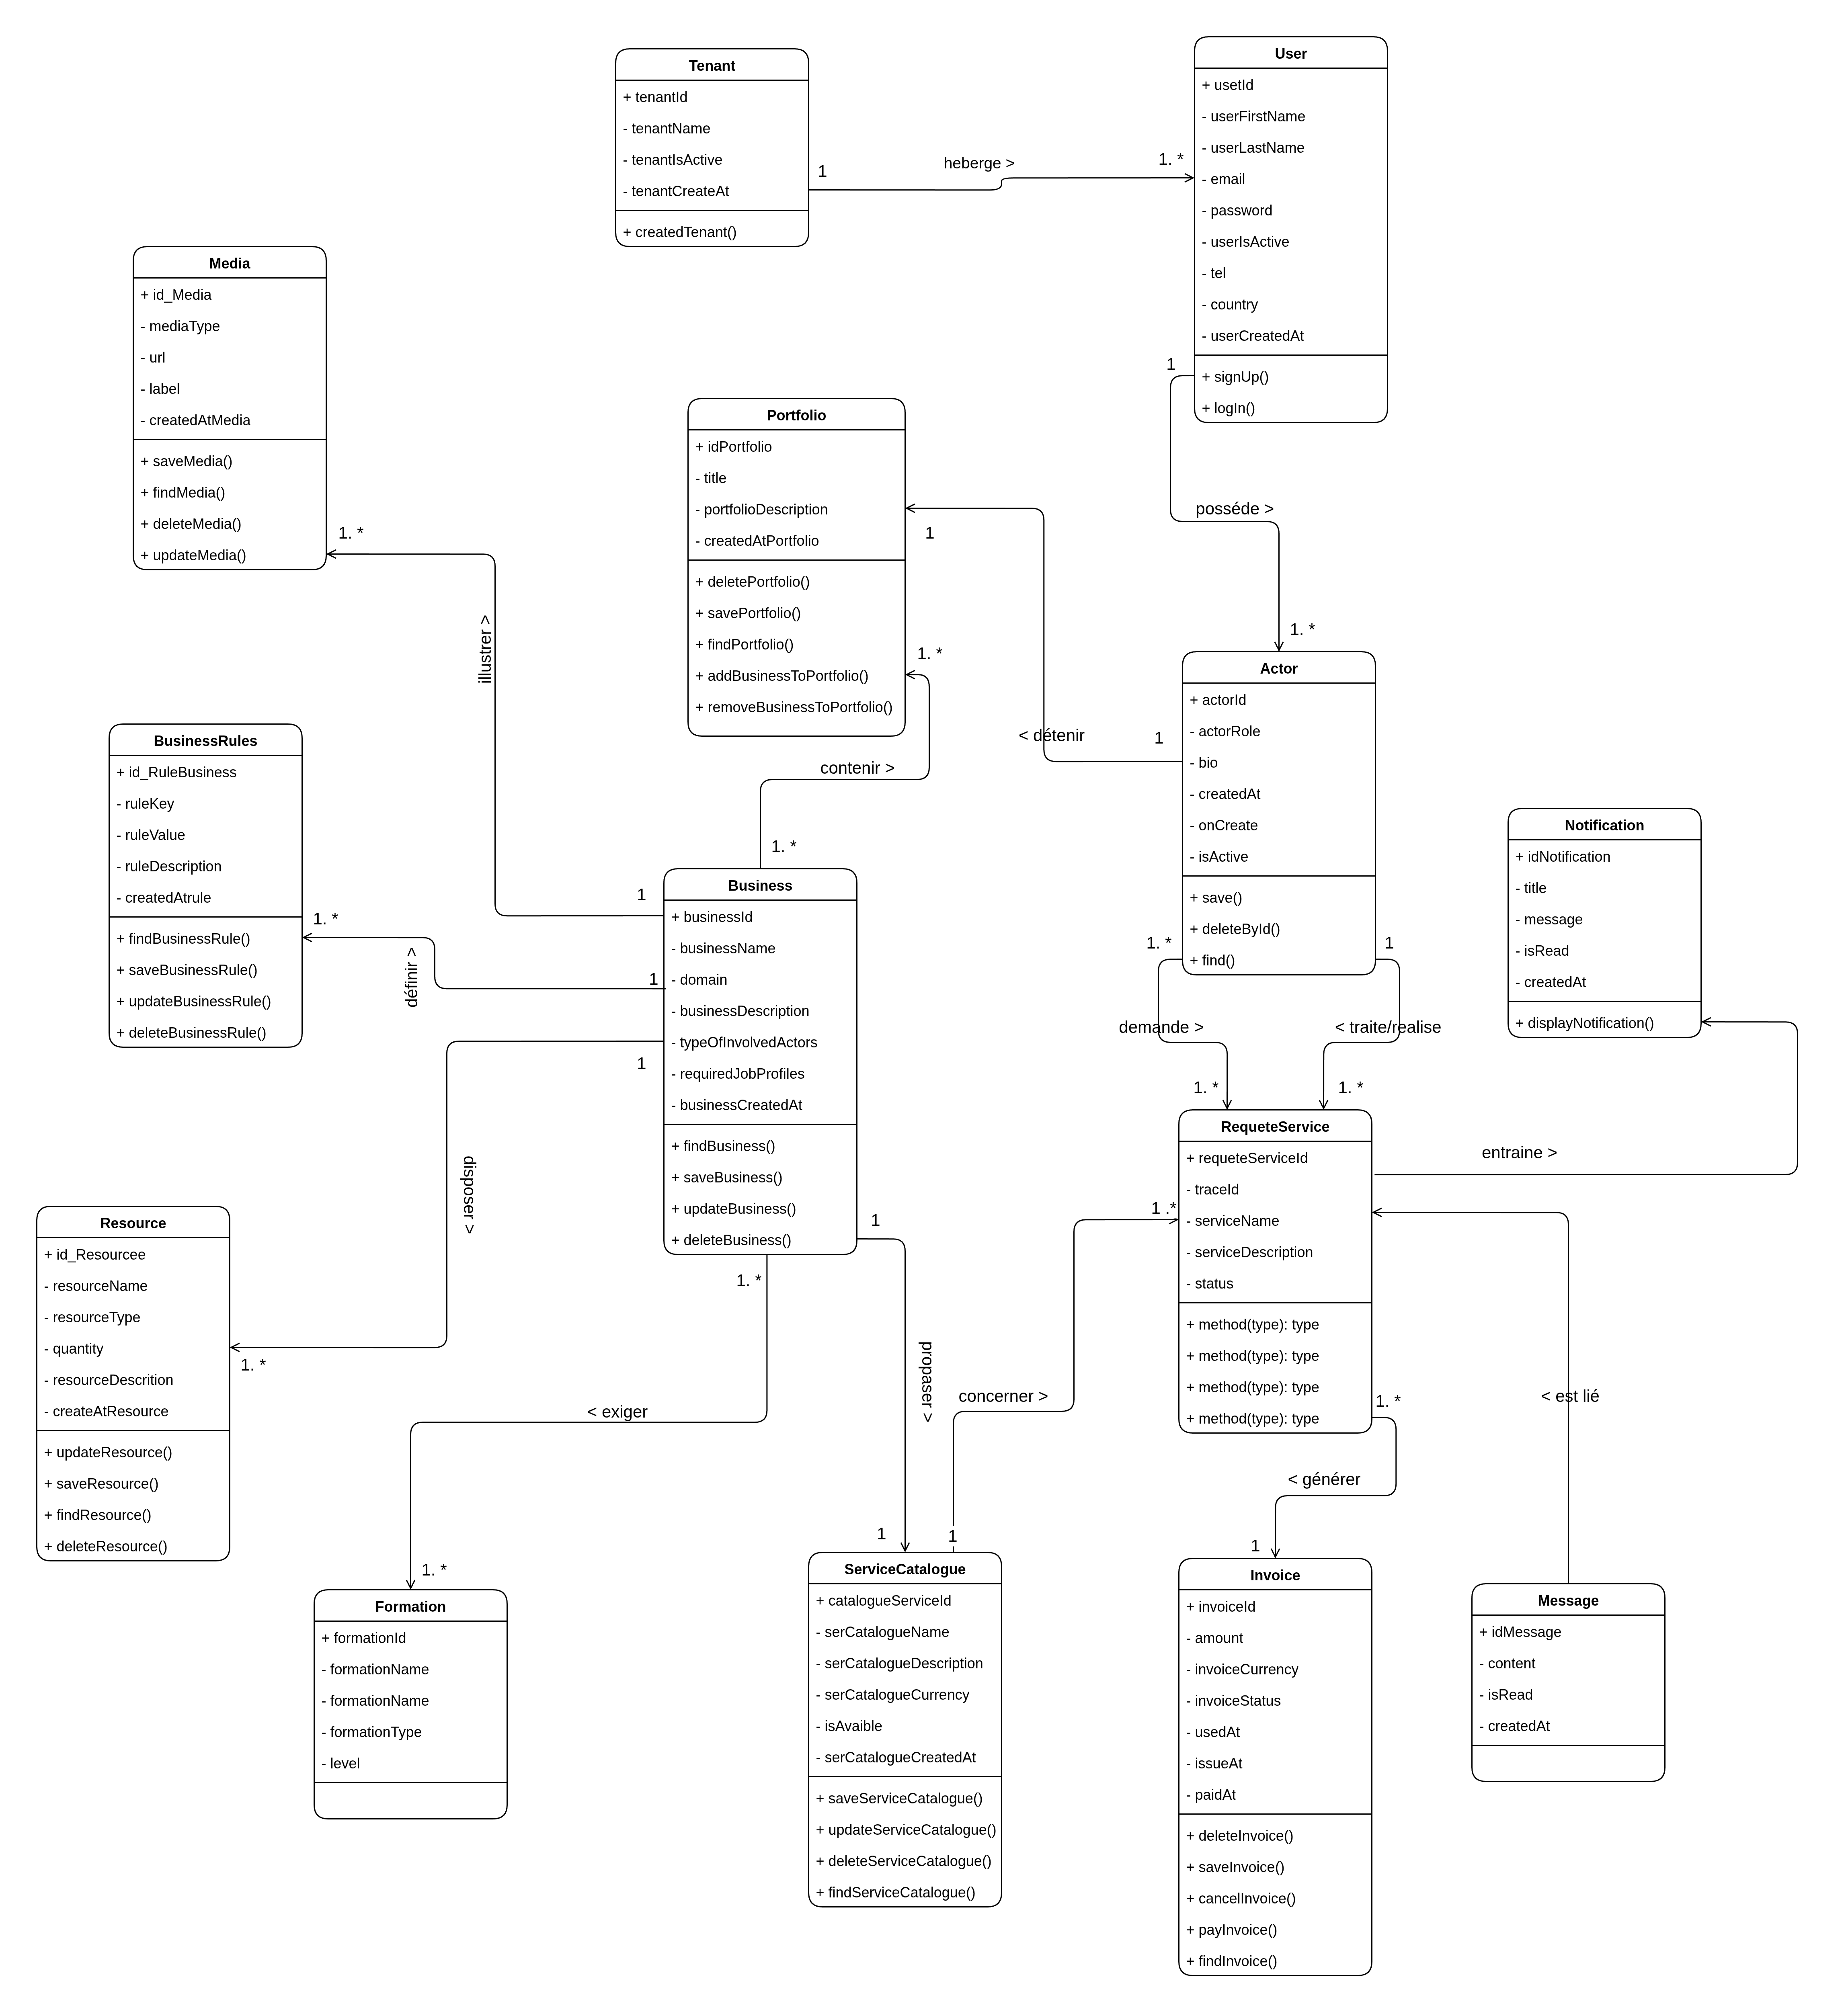
\includegraphics[width=0.8\linewidth]{chapitres/CLASSES (2) (1).drawio.png}
    \captionof{figure}{Diagramme de classes métier de BCaaS}
    \label{fig:placeholder}
\end{figure}
\label{fig:classes}

\section{Contraintes d'intégrité}

Le tableau~\ref{tab:integrite} liste les principales contraintes d'intégrité
référentielle et d'unicité.

\begin{table}[H]
\centering
\caption{Principales contraintes d'intégrité}
\label{tab:integrite}
\renewcommand{\arraystretch}{1.25}\footnotesize
\begin{tabularx}{\linewidth}{L{4cm} L{2.4cm} X}
\toprule
\textbf{Table} & \textbf{Type} & \textbf{Description} \\
\midrule
tenants            & Unique      & Nom de tenant unique \\
users              & Unique      & Email unique \\
users              & FK          & \texttt{tenant\_id} $\to$ tenants \\
portfolios         & Unique + FK & Un portfolio par acteur \\
service\_requests  & FK          & consumer, provider, catalogue, tenant existants \\
invoices           & Unique + FK & Une facture par demande de service \\
messages, notifications, audit\_events & FK (NOT NULL) & \texttt{tenant\_id} obligatoire \\
\bottomrule
\end{tabularx}
\end{table}

\section{Machines à états}

Deux entités portent une machine à états explicite. La \texttt{ServiceRequest} suit le
cycle \texttt{PENDING} $\to$ \texttt{ACCEPTED} $\to$ \texttt{IN\_PROGRESS} $\to$
\texttt{FULFILLED}, avec \texttt{CANCELLED} accessible depuis tout état non terminal ;
chaque transition horodate un champ dédié (\texttt{requestedAt}, \texttt{acceptedAt},
\texttt{startedAt}, \texttt{fulfilledAt}, \texttt{cancelledAt}). La transition
\texttt{fulfill} déclenche la génération automatique de l'\texttt{Invoice}. La facture
suit quant à elle \texttt{PENDING} $\to$ \texttt{PAID} ou \texttt{CANCELLED}.

% \figplaceholder{Diagrammes d'états-transitions UML : (a) ServiceRequest
% (PENDING/ACCEPTED/IN\_PROGRESS/FULFILLED/CANCELLED) ; (b) Invoice (PENDING/PAID/CANCELLED).}{5.5cm}

% \begin{figure}[H]
%   \centering
%   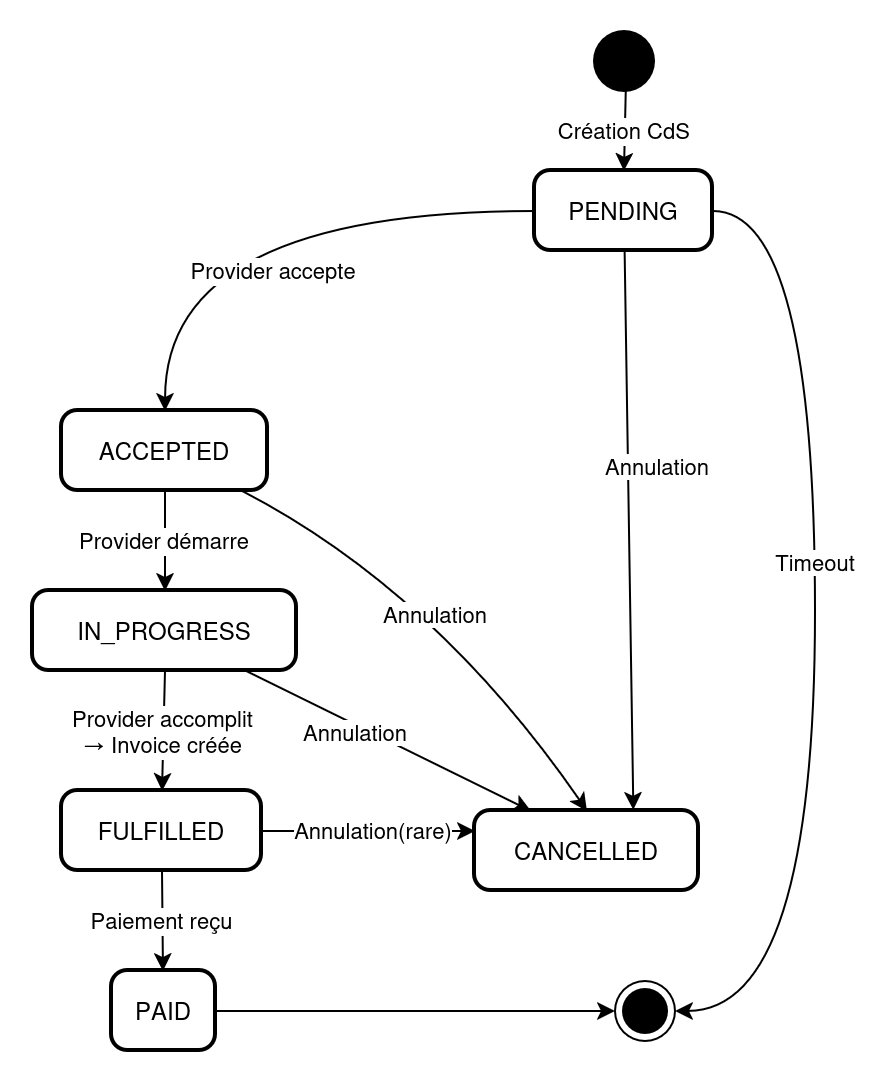
\includegraphics[width=0.6\textwidth]{figures/diagrammes/ETAT_SERVICE_REQUEST.drawio.png}
%   \caption{Machines à états de \texttt{ServiceRequest}.}
%   \label{fig:etatsr}
% \end{figure} 

% \begin{figure}[H]
%   \centering
%   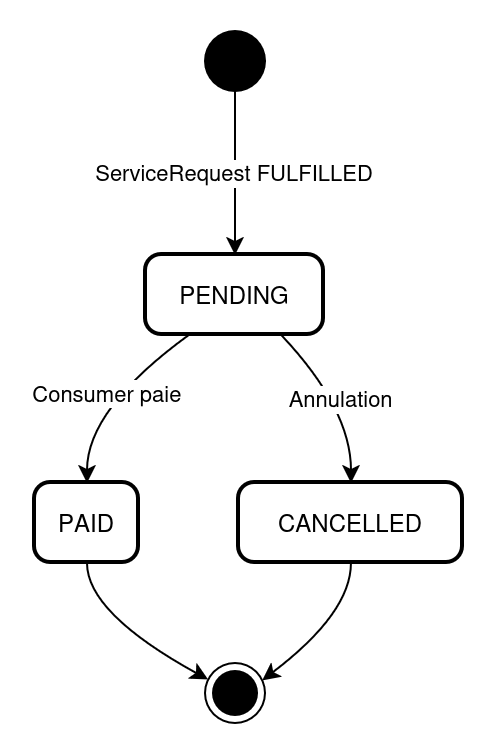
\includegraphics[width=0.4\textwidth]{figures/diagrammes/ETAT_INVOICE.drawio.png}
%   \caption{Machines à états de \texttt{INVOICE}.}
%   \label{fig:etatinvoice}
% \end{figure}

\begin{figure}[H]
  \centering
  \begin{minipage}{0.55\textwidth}
    \centering
    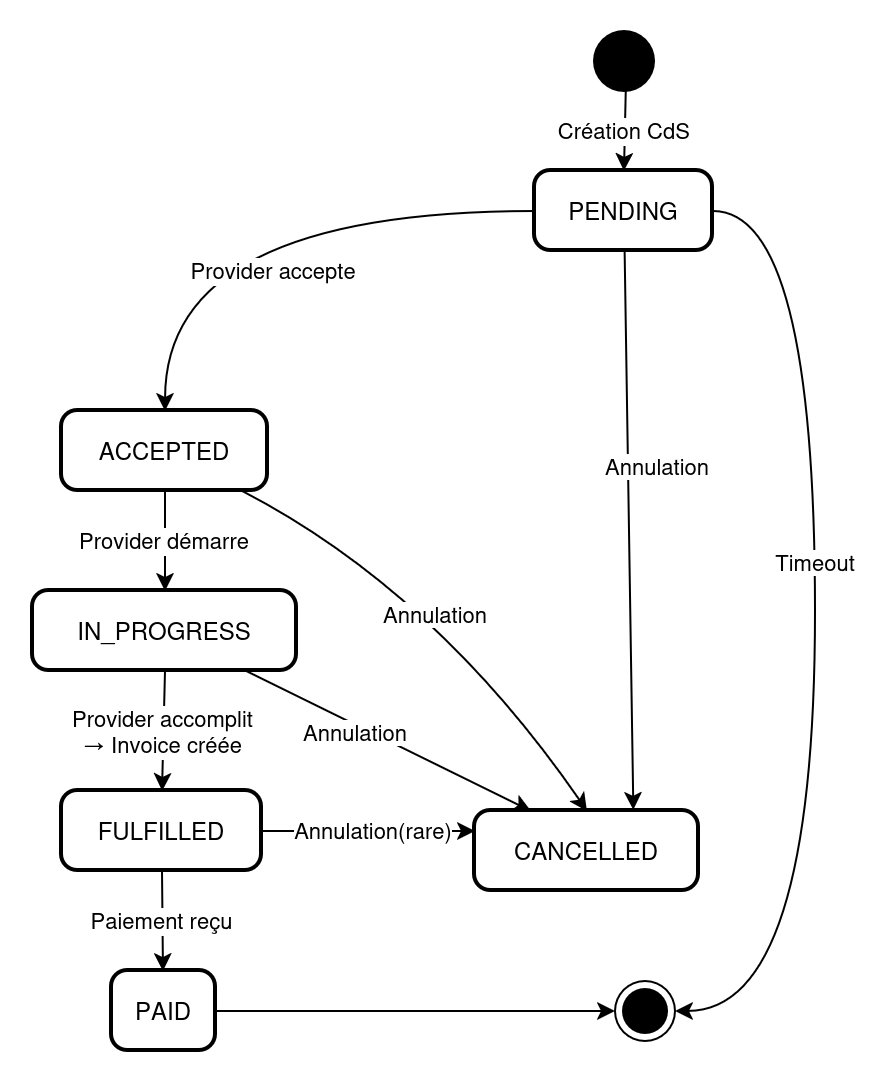
\includegraphics[width=\textwidth]{figures/diagrammes/ETAT_SERVICE_REQUEST.drawio.png}
    \caption{Machine à états de \texttt{ServiceRequest}}
    \label{fig:etatsr}
  \end{minipage}
  \hfill
  \begin{minipage}{0.38\textwidth}
    \centering
    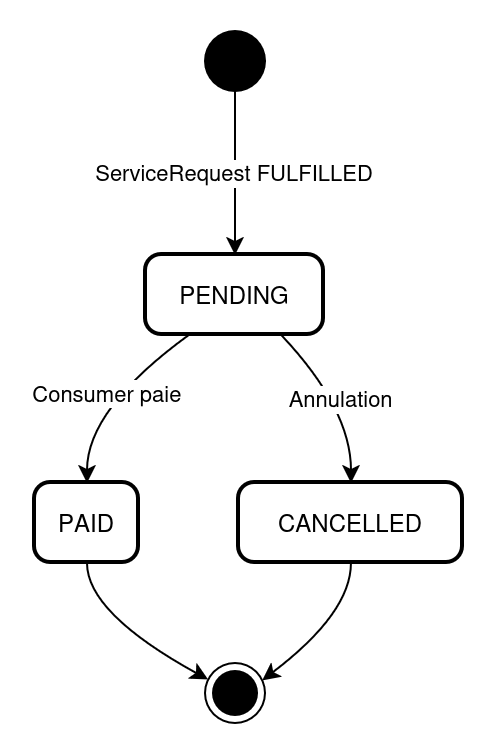
\includegraphics[width=\textwidth]{figures/diagrammes/ETAT_INVOICE.drawio.png}
    \caption{Machine à états de \texttt{Invoice}}
    \label{fig:etatinvoice}
  \end{minipage}
\end{figure}
\chapter{Implémentation technique}
\label{chap:impl}

\section{Pile technologique}

Le tableau~\ref{tab:pile} présente la pile effectivement utilisée. Conformément au cadrage
MVP retenu, les versions et composants y sont indiqués tels qu'ils sont réellement mis en
œuvre ; les briques avancées non câblées sont reportées au chapitre~\ref{chap:perspectives}.

\begin{table}[H]
\centering
\caption{Pile technologique de BCaaS}
\label{tab:pile}
\renewcommand{\arraystretch}{1.25}\footnotesize
\begin{tabularx}{\linewidth}{L{4.2cm} X L{2.8cm}}
\toprule
\textbf{Composant} & \textbf{Technologie} & \textbf{Version} \\
\midrule
Framework backend     & Spring Boot (servlet, MVC)         & 3.5.x \\
Langage               & Java                               & 21 LTS \\
Base de données       & PostgreSQL                         & 16 \\
Migrations            & Liquibase                          & 4.x \\
Sécurité              & Spring Security + JWT (jjwt)       & 0.12.6 \\
Documentation API     & SpringDoc OpenAPI                  & 2.8.6 \\
Cache / pub-sub       & Redis                              & 7 \\
Bus d'événements      & Apache Kafka (infra)               & 7.6 (image) \\
Build                 & Maven                              & 3.9+ \\
Tests                 & JUnit 5 + Mockito + AssertJ        & 152 tests \\
Conteneurisation      & Docker + Docker Compose            & --- \\
Frontend              & Next.js / React / TypeScript       & 16 / 19 \\
\bottomrule
\end{tabularx}
\end{table}

\section{Structure du projet}

Le projet suit l'architecture hexagonale combinée au DDD. L'arborescence backend est
organisée par responsabilités techniques au sein du package \texttt{com.bizcore.bizcore\_backend}.

\begin{lstlisting}[language={},caption={Structure du projet backend},captionpos=b]
src/main/java/com/bizcore/bizcore_backend/
  +-- auth/         # Authentification (register, login, roles)
  +-- config/       # Configurations (Kafka, Redis, Security, cache)
  +-- controller/   # Controllers REST
  +-- domain/       # Entites JPA (15) + enum SupportedCurrency
  +-- dto/          # Objets de transfert
  +-- exception/    # GlobalExceptionHandler, ApiError
  +-- listener/     # Listener Kafka (consommateur)
  +-- repository/   # Repositories Spring Data (tenant-aware)
  +-- security/     # JwtService, JwtAuthFilter, TenantFilter, TenantContext
  +-- service/      # Services metier
src/main/resources/
  +-- application.properties
  +-- db/changelog/ # Migrations Liquibase
src/test/           # 16 classes, 152 tests (JUnit 5 + Mockito)
\end{lstlisting}

\section{Multi-tenant et isolation}

L'isolation repose sur le modèle « schéma partagé, colonne \texttt{tenant\_id} » et sur
trois pièces coordonnées.

\paragraph{1. \texttt{TenantContext} --- un \texttt{ThreadLocal}.}
Chaque requête HTTP dispose d'une copie isolée du tenant actif, stockée dans un
\texttt{ThreadLocal<UUID>}, ce qui évite toute fuite entre requêtes concurrentes partageant
le même pool de threads.

\paragraph{2. \texttt{TenantFilter} --- extraction depuis le JWT.}
Filtre \texttt{OncePerRequestFilter} d'ordre $2$ (après le filtre d'authentification), il
lit le claim \texttt{tenantId} du JWT et le place dans le contexte, puis le purge dans un
bloc \texttt{finally}.

\begin{lstlisting}[language=Java,caption={Extrait simplifié de TenantFilter},captionpos=b]
String tenantIdStr = jwtService.extractTenantId(jwt);   // claim "tenantId"
TenantContext.setTenantId(UUID.fromString(tenantIdStr));
try {
    filterChain.doFilter(request, response);
} finally {
    TenantContext.clear();   // pas de fuite inter-tenant
}
\end{lstlisting}

\paragraph{3. Injection du claim à la connexion.}
À l'authentification, \texttt{JwtService} embarque \texttt{tenantId} et \texttt{tenantName}
dans le token. Le tenant est ainsi dérivé de l'utilisateur (colonne \texttt{users.tenant\_id})
et relu à chaque requête sans appel supplémentaire à la base. L'isolation est appliquée
dans la couche service via des requêtes \emph{tenant-aware} de type
\texttt{findAllByTenantId(...)}.

\begin{garantie}[Garantie d'isolation et limite assumée]
Le \texttt{tenant\_id} circule dans le contexte d'exécution et conditionne les requêtes des
services principaux ; un générateur de clés de cache préfixe par tenant. \textbf{Limite
assumée :} l'isolation n'est pas une barrière globale (ni filtre Hibernate
\texttt{@Filter}, ni \emph{Row-Level Security} PostgreSQL) ; elle repose sur la discipline
de chaque méthode de service. Le renforcement de cette barrière est traité au
chapitre~\ref{chap:perspectives}.
\end{garantie}

\section{Sécurité : JWT et RBAC}

L'authentification repose sur un couple email / mot de passe chiffré par BCrypt. Le token
JWT, signé en HMAC-SHA, porte les rôles et le \texttt{tenantId}. Le contrôle d'accès est
basé sur les rôles (\texttt{USER}, \texttt{ADMIN}, \texttt{PROVIDER}, \texttt{CONSUMER}),
un même utilisateur pouvant cumuler plusieurs rôles. Spring Security joue ici le rôle d'un
pare-feu applicatif filtrant les requêtes selon l'analogie du tableau~\ref{tab:correspondance}.

\section{Persistance et migrations}

Le schéma est géré par Liquibase, garantissant des migrations versionnées et reproductibles
(création du schéma, ajout des tables \texttt{notifications}, \texttt{messages},
\texttt{audit\_events}, colonnes \texttt{tenant\_id} contraintes par clé étrangère et
indexées). Le paramètre \texttt{ddl-auto=none} laisse Liquibase seul maître du schéma en
exécution.

\section{Temps réel et événementiel}

La messagerie instantanée sur les demandes de service est réalisée par \textbf{Redis
publish/subscribe} : le service de messages publie sur un canal
\texttt{messages:<requestId>}. Un \textbf{bus d'événements Kafka} est configuré
(\texttt{KafkaTemplate} côté producteur, \texttt{@KafkaListener} sur le topic
\texttt{bizcore.events} côté consommateur) ; l'infrastructure est posée et le consommateur
opérationnel, la \emph{production} d'événements restant à câbler (perspective au
chapitre~\ref{chap:perspectives}). Le cache Redis est de même configuré (gestionnaire de
cache, TTL par espace) et prêt à être activé par annotations.

\section{Documentation et conteneurisation}

L'API est documentée automatiquement via SpringDoc OpenAPI et explorable par Swagger UI
(annexe~\ref{ann:swagger}). Un \texttt{docker-compose} décrit l'environnement local complet
(application, PostgreSQL, Redis, Kafka avec \emph{healthchecks} et dépendances
ordonnancées) ; en production, l'API et sa base s'exécutent sur Render.

\chapter{Protocole d'échange pour un cas métier concret}
\label{chap:protocole}

Pour illustrer la « pensée protocolaire » du projet, ce chapitre formalise l'échange d'un
cas métier complet --- la création d'un \texttt{Business} puis l'ajout d'un service à son
catalogue --- comme on spécifierait un protocole réseau : en-têtes obligatoires, payload,
réponses, codes d'erreur et sémantique de transport.

\section{Cas choisi : création d'un Business et ajout au catalogue}

Ce cas correspond à deux requêtes distinctes mais liées, typiques de l'enregistrement d'une
nouvelle activité (auto-école, cabinet de conseil, etc.) dans un tenant.

\section{Protocole : création d'un Business}

\noindent\textbf{Endpoint :} \texttt{POST /api/businesses}\\
\textbf{En-têtes obligatoires :}
\begin{itemize}
  \item \texttt{Authorization: Bearer <JWT>} --- authentification (analogie : ticket de
        session) ; le claim \texttt{tenantId} joue le rôle de l'adresse réseau.
\end{itemize}

\begin{lstlisting}[language=json,caption={Corps de la requête (payload)},captionpos=b]
 
{
  "name": "Auto-Ecole Centrale",
  "domain": "driving_school",
  "description": "Numero 1 dans la formation auto",
  "typeOfInvolvedActors": ["instructor", "student"],
  "requiredJobProfile": "moniteur",
  "tenantId": "3fa85f64-5717-4562-b3fc-2c963f66afa6"
}
\end{lstlisting}

\begin{lstlisting}[language=json,caption={Réponse (succès 201 Created)},captionpos=b]
{
  "id": "550e8400-e29b-41d4-a716-446655440000",
  "name": "Auto-Ecole Centrale",
  "domain": "driving_school",
  "createdAt": "2025-05-04T10:00:00Z"
}
\end{lstlisting}

\paragraph{Codes d'erreur (analogie : messages ICMP).}
\begin{itemize}
  \item \texttt{400 Bad Request} : payload invalide ;
  \item \texttt{401 Unauthorized} : JWT manquant ou invalide ;
  \item \texttt{403 Forbidden} : rôle insuffisant ;
  \item \texttt{404 Not Found} : ressource inexistante ;
  \item \texttt{409 Conflict} : ressource déjà existante.
\end{itemize}

\section{Protocole : ajout au catalogue de services}

\noindent\textbf{Endpoint :} \texttt{POST /api/service-catalogues/business/\{businessId\}}\\
\textbf{En-têtes :} identiques, plus une corrélation optionnelle.

\begin{lstlisting}[language=json,caption={Corps de la requête},captionpos=b]
{
  "name": "Cours de conduite",
  "description": "Formation theorique et pratique de 3 mois",
  "basePrice": 150000,
  "currency": "XAF",
  "isAvailable": true
}
\end{lstlisting}

\paragraph{Sémantique du transport.}
\begin{itemize}
  \item \textbf{Mode :} synchrone (REST) --- analogie TCP (fiable, ordonné) ;
  \item \textbf{Timeout :} de l'ordre de 30 secondes ;
  \item \textbf{Idempotence :} non (chaque \texttt{POST} crée une nouvelle ressource) ;
  \item \textbf{Retry :} recommandé avec \emph{backoff} exponentiel (au plus 3 tentatives).
\end{itemize}

% \section{Diagramme de séquence}

% \figplaceholder{Diagramme de séquence UML du cas « création Business + ajout au catalogue » :
% acteurs Provider, API Gateway, TenantFilter, BusinessService, ServiceCatalogueService, base
% de données ; messages REST et réponses 201, propagation du traceId.}{6.5cm}
% \captionof{figure}{Diagramme de séquence du cas métier « Business + Catalogue »}
% \label{fig:sequence}

\chapter{Traçabilité et observabilité}
\label{chap:observ}

Dans une architecture multi-tenant et distribuée comme la plateforme BCaaS, l'absence de visibilité sur l'état interne du système constitue un risque majeur. Pour garantir une transparence totale sur le cycle de vie des transactions, ce chapitre formalise notre couche d'observabilité.

En transposant les techniques de supervision et d'analyse de protocoles propres aux infrastructures réseaux --- à l'image d'une capture de flux ou d'une analyse de paquets sous Wireshark --, nous articulons ce module autour d'éléments réellement implémentés au cœur de l'application :
\begin{enumerate}
    \item \textbf{Une piste d'audit :} Matérialisée par l'entité \texttt{AuditEvent}, elle enregistre de manière exhaustive les actions clés, les adresses IP et les dimensions de sécurité de chaque transaction.
    \item \textbf{Un système de tracing distribué :} L'utilisation des identifiants \texttt{traceId} et \texttt{correlationId} (UUID) qui se propagent dans tout le système pour suivre les flux de bout en bout, jouant le rôle des numéros de séquence TCP.
    \item \textbf{Un service analytique :} Un module dédié exposé par API pour calculer les indicateurs clés (KPIs) des tenants, calqués sur les métriques réseaux fondamentales (latence moyenne, débit, taux d'erreur).
\end{enumerate}

Ce dispositif se trouve complété en fin de chapitre par une proposition d'intégration de logs structurés au format JSON.

\section{Piste d'audit}

L'entité \texttt{AuditEvent} enregistre les événements significatifs du système : type d'entité concernée (\texttt{SERVICE\_REQUEST}, \texttt{INVOICE}, \texttt{ACTOR}, \texttt{BUSINESS}, \texttt{SERVICE\_CATALOGUE}), action (\texttt{CREATED}, \texttt{STATUS\_CHANGED}, \texttt{UPDATED}, \texttt{DELETED}), statut précédent et nouveau, adresse IP, \emph{user agent} et métadonnées au format JSON. 

Conçue selon un principe de stricte \textbf{immuabilité}, la piste d'audit fonctionne exclusivement en mode \emph{Append-Only} (écriture seule) : aucune opération de mise à jour (\texttt{UPDATE}) ou de suppression (\texttt{DELETE}) n'est exposée par l'API ou autorisée par le système, garantissant la non-répudiation des logs même en cas de compromission d'un administrateur de tenant.

L'enregistrement capture les dimensions clés de chaque transaction :
\begin{itemize}
  \item \textbf{Le contexte d'application} : Le type d'entité concernée.
  \item \textbf{La nature de l'opération} : L'action effectuée, accompagnée de l'état précédent et du nouvel état de l'entité.
  \item \textbf{L'empreinte d'infrastructure} : L'adresse IP de l'appelant ainsi que son \emph{user agent} (navigateur ou client applicatif).
  \item \textbf{La charge utile} : Des métadonnées dynamiques stockées dans un champ au format \texttt{JSONB} sous PostgreSQL. Ce choix technique permet de supporter un polymorphisme des données métiers (les métadonnées d'une facture différant de celles d'un catalogue) sans altérer le schéma relationnel.
\end{itemize}

Chaque événement porte obligatoirement les identifiants bruts \texttt{tenantId}, \texttt{actorId}, \texttt{entityId} et \texttt{traceId}. L'API d'audit permet d'interroger et de filtrer ces événements par demande de service, par acteur, par tenant et par trace.

\begin{analogie}[Analogie : Deep Packet Inspection et Sonde Réseau]
La capture des données d'audit est réalisée de manière non intrusive via un intercepteur applicatif (\texttt{OncePerRequestFilter} au niveau de la couche de sécurité), agissant comme une sonde réseau (SPAN/Mirroring). L'analyse de la charge utile \texttt{JSONB} est analogue au \emph{Deep Packet Inspection} (DPI), où l'on inspecte non seulement les en-têtes du paquet (IP, Tenant, Acteur), mais également le contenu profond de la charge utile applicative pour en valider l'intégrité opérationnelle.
\end{analogie}

\section{Tracing : \texttt{traceId} et \texttt{correlationId}}

Chaque \texttt{ServiceRequest} véhicule de manière intrinsèque un \texttt{traceId} et un \texttt{correlationId} sous forme d'identifiants uniques universels (UUID). Bien qu'ils concourent tous deux à la visibilité du système, ils répondent à des granularités distinctes :
\begin{itemize}
    \item \textbf{\texttt{traceId}} : Il est associé à une unique requête HTTP entrante. Il permet de suivre le fil d'exécution synchrone d'un bout à l'autre des couches logicielles (\emph{Controller}, \emph{Service}, \emph{Repository}) pour une opération donnée.
    \item \textbf{\texttt{correlationId}} : Il englobe une opération métier globale pouvant impliquer plusieurs requêtes ou événements asynchrones distincts (par exemple, une demande de service qui déclenche une génération de facture puis une notification). Toutes ces sous-opérations partagent le même \texttt{correlationId}, permettant de lier logiquement des transactions hétérogènes.
\end{itemize}

Le mécanisme repose sur la \textbf{propagation de contexte}. À l'entrée du système, la passerelle applicative gère la genèse de ces identifiants et les injecte dans les en-têtes HTTP (\texttt{X-Trace-Id} et \texttt{X-Correlation-Id}). Les services internes extraient ces en-têtes et les rattachent au fil d'exécution via le mécanisme \texttt{MDC} (\emph{Mapped Diagnostic Context}) de la brique de journalisation, garantissant leur inscription systématique dans chaque log généré.

\begin{analogie}[Analogie : En-tête de protocole et circuit virtuel]
Le \texttt{traceId} et le \texttt{correlationId} agissent exactement comme les en-têtes de contrôle d'un protocole réseau (tels que les numéros de séquence TCP ou les étiquettes MPLS). Au lieu d'altérer la charge utile de la requête métier, ces identifiants sont encapsulés dans les couches de transport applicatif (en-têtes HTTP), permettant aux routeurs applicatifs et aux commutateurs de logs de corréler et de reconstituer la topologie complète du flux de données sans inspecter le contenu sémantique du message.
\end{analogie}

\section{Analytique et KPIs}

Le service d'analytique calcule en temps réel, pour chaque tenant, les indicateurs clés de performance (KPIs) formalisés au chapitre~\ref{chap:math}. Afin de préserver les performances du noyau transactionnel et d'éviter des requêtes d'agrégation (\texttt{COUNT}, \texttt{SUM}) lourdes sur la base de données relationnelle, le système implémente un principe de \textbf{séparation des responsabilités} (CQRS applicatif). Les métriques sont soit calculées de manière asynchrone au fil de l'eau via le bus d'événements, soit agrégées et matérialisées dans un cache en mémoire à haute disponibilité (\texttt{Redis}).

L'endpoint \texttt{GET /api/analytics/tenants/\{tenantId\}/kpis} expose ces indicateurs. Pour garantir une haute réactivité, les réponses de cet endpoint sont associées à une durée de vie stricte (\emph{TTL - Time To Live}), limitant la fréquence de recalcul. Le tableau~\ref{tab:metriques} dresse la liste de ces métriques opérationnelles et explicite leur équivalent conceptuel dans le domaine des réseaux.

\begin{table}[H]
\centering
\caption{Métriques de BCaaS et leur analogie réseau}
\label{tab:metriques}
\renewcommand{\arraystretch}{1.25}\footnotesize
\begin{tabularx}{\linewidth}{L{3.6cm} L{4.4cm} X}
\toprule
\textbf{Métrique} & \textbf{Analogie réseau} & \textbf{Calcul} \\
\midrule
Taux de conversion   & Taux de livraison de paquets & demandes finalisées / total \\
Latence moyenne      & RTT (Round Trip Time)        & temps moyen de traitement \\
Débit (req/s)        & Bande passante               & requêtes par minute \\
Taux d'erreur        & Taux de perte                & réponses 4xx/5xx / total \\
Panier moyen         & Taille moyenne de payload    & chiffre d'affaires / nb factures \\
Délai d'exécution    & Délai de routage             & temps requête $\rightarrow$ finalisation \\
\bottomrule
\end{tabularx}
\end{table}

\begin{analogie}[Analogie : Cache DNS et TTL]
Le mécanisme de mise en cache des KPIs avec un TTL (Time To Live) est rigoureusement identique à la gestion d'un cache DNS ou d'une table de routage dynamique. Un équipement réseau ne sollicite pas le serveur racine pour chaque paquet à acheminer ; il maintient une copie locale des routes et des résolutions de noms pendant une durée déterminée afin de maximiser le débit global et de minimiser la surcharge CPU du système.
\end{analogie}

\section{Logs structurés (proposition)}

Pour compléter le dispositif d'observabilité, une stratégie de journalisation structurée au format JSON est proposée. Contrairement aux chaînes de caractères de texte brut traditionnelles (\emph{Plain Text}) dont l'analyse logicielle requiert des expressions régulières complexes et fragiles, le format JSON standardise nativement la sémantique de chaque ligne de log. Chaque entrée intègre systématiquement le contexte d'exécution complet : \texttt{tenant\_id}, \texttt{trace\_id}, \texttt{actor\_id}, le nom du service, l'opération exécutée, la durée exacte du traitement et le code de statut HTTP retourné.

L'implémentation de cette proposition repose sur un découplage total : l'application écrit ces objets JSON directement sur la sortie standard (\texttt{STDOUT}), minimisant l'impact sur le thread d'exécution métier. Un agent de collecte léger (tel que \emph{Promtail} ou \emph{FluentBit}) se charge ensuite d'aspirer ces flux de manière asynchrone pour alimenter une chaîne de centralisation (\emph{Grafana Loki} ou pile \emph{ELK}). Cette structuration permet d'effectuer des requêtes multi-critères instantanées et de corréler une alerte de performance globale avec les logs spécifiques d'un tenant.

\begin{analogie}[Analogie : Protocoles d'export de flux (NetFlow / IPFIX)]
La journalisation structurée en JSON is l'équivalent applicatif des protocoles de métrologie réseau tels que \emph{NetFlow} (Cisco) ou \emph{IPFIX}. Un routeur réseau n'exporte pas des lignes de texte brut pour décrire le trafic ; il transmet des enregistrements structurés contenant des champs normalisés (adresses IP, ports, drapeaux TCP, volumes). Cette standardisation permet aux collecteurs réseau, tout comme à nos indexeurs de logs, d'agréger, de filtrer et de cartographier le trafic en temps réel à grande échelle.
\end{analogie}

\chapter{Frontend et déploiement}
\label{chap:frontend}

\section{Architecture du frontend}

Le frontend est développé avec Next.js (App Router) et React en TypeScript. L'architecture de l'interface se structure autour d'un site vitrine public, exposant l'approche protocolaire, la documentation interactive de la plateforme et les guides de démarrage. Un tableau de bord d'administration, permettant aux acteurs authentifiés de piloter les demandes de service et de gérer les acteurs, est prévu dans une version future.

\section{Choix techniques}

Le choix de Next.js est motivé par sa capacité à combiner le rendu côté serveur (\emph{Server-Side Rendering} - SSR) pour la sécurisation des tableaux de bord dynamiques, et la génération statique (\emph{Static Site Generation} - SSG) pour maximiser les performances de chargement du site vitrine. Le tableau~\ref{tab:frontend} dresse la cartographie logicielle de l'interface et ses justifications.

\begin{table}[H]
\centering
\caption{Technologies du frontend et leur rôle architectural}
\label{tab:frontend}
\renewcommand{\arraystretch}{1.25}\footnotesize
\begin{tabularx}{\linewidth}{L{3.6cm} L{4.2cm} X}
\toprule
\textbf{Besoin} & \textbf{Technologie} & \textbf{Justification} \\
\midrule
Framework        & Next.js 16 (App Router) & SSR/SSG, optimisation du TTFB, routage par dossier \\
UI               & React 19 + TypeScript   & Composants typés, gestion robuste des états d'affichage \\
Styling          & Tailwind CSS 3          & Conception atomique, design système fluide \\
Composants       & Radix UI                & Primitives de composants hautement accessibles \\
Animations / 3D  & Framer Motion, react-three/fiber & Restitution immersive de la métaphore réseau \\
État global      & Zustand                 & Store centralisé léger, découplé du cycle de rendu React \\
Données serveur  & TanStack Query + Axios    & Gestion du cache local et synchronisation asynchrone avec l'API \\
\bottomrule
\end{tabularx}
\end{table}

La couche de communication du frontend est construite avec Axios et encapsulée dans TanStack Query pour la synchronisation des données. Un intercepteur Axios injecte automatiquement le jeton JWT d'authentification sur chaque requête sortante. L'injection des en-têtes de tracing distribué (\texttt{X-Trace-Id}, \texttt{X-Correlation-Id}) est prévue dans une version ultérieure.

\section{Pages principales}

Les routes implémentées au sein de l'application comprennent :
\begin{itemize}
    \item \textbf{Espace public} : La page d'accueil (\texttt{/}), la démonstration interactive du protocole (\texttt{/demo}), l'assistant conversationnel d'assistance (\texttt{/chat}), la documentation technique (\texttt{/docs}, \texttt{/docs/[id]}) et les guides d'intégration (\texttt{/guides}, \texttt{/guides/[slug]}).
    \item \textbf{Espace d'administration (à venir)} : Tableau de bord central (\texttt{/dashboard}) et sous-pages spécialisées : gestion des demandes (\texttt{/dashboard/requests}), des acteurs (\texttt{/dashboard/actors}), des règles métiers (\texttt{/dashboard/businesses}), de la facturation (\texttt{/dashboard/invoices}), des catalogues de services (\texttt{/dashboard/services}) et des paramètres globaux (\texttt{/dashboard/settings}). Les ébauches de ces pages sont présentes dans le code mais leur intégration fonctionnelle complète est repoussée à une version ultérieure.
\end{itemize}

\section{Déploiement}

L'infrastructure applicative adopte une topologie de déploiement multi-cloud distribuée pour optimiser les coûts et isoler les responsabilités d'exécution :
\begin{itemize}
    \item \textbf{Couche Backend et Persistance} : L'API Spring Boot et la base de données relationnelle PostgreSQL sont déployées sur la plateforme \textbf{Render} (\url{https://bizcore-api.onrender.com}). La documentation interactive des points d'accès (Swagger UI) y est directement hébergée et accessible pour les tests d'intégration.
    \item \textbf{Couche Frontend} : Le serveur de rendu Next.js et l'interface utilisateur sont déployés sur la plateforme \textbf{Vercel} (\url{https://bizcore-liard.vercel.app}), bénéficiant nativement d'un réseau de diffusion de contenu (CDN) mondial pour minimiser la latence réseau lors du téléchargement des ressources statiques.
\end{itemize}

La sécurité des communications entre ces deux environnements distants est assurée par le chiffrement systématique des flux via le protocole TLS (HTTPS) et par la configuration d'une politique de filtrage de ressources partagées (CORS) stricte sur l'API Spring Boot, restreignant les accès légitimes au seul domaine du frontend.

  
\begin{figure}[H]
    \centering
    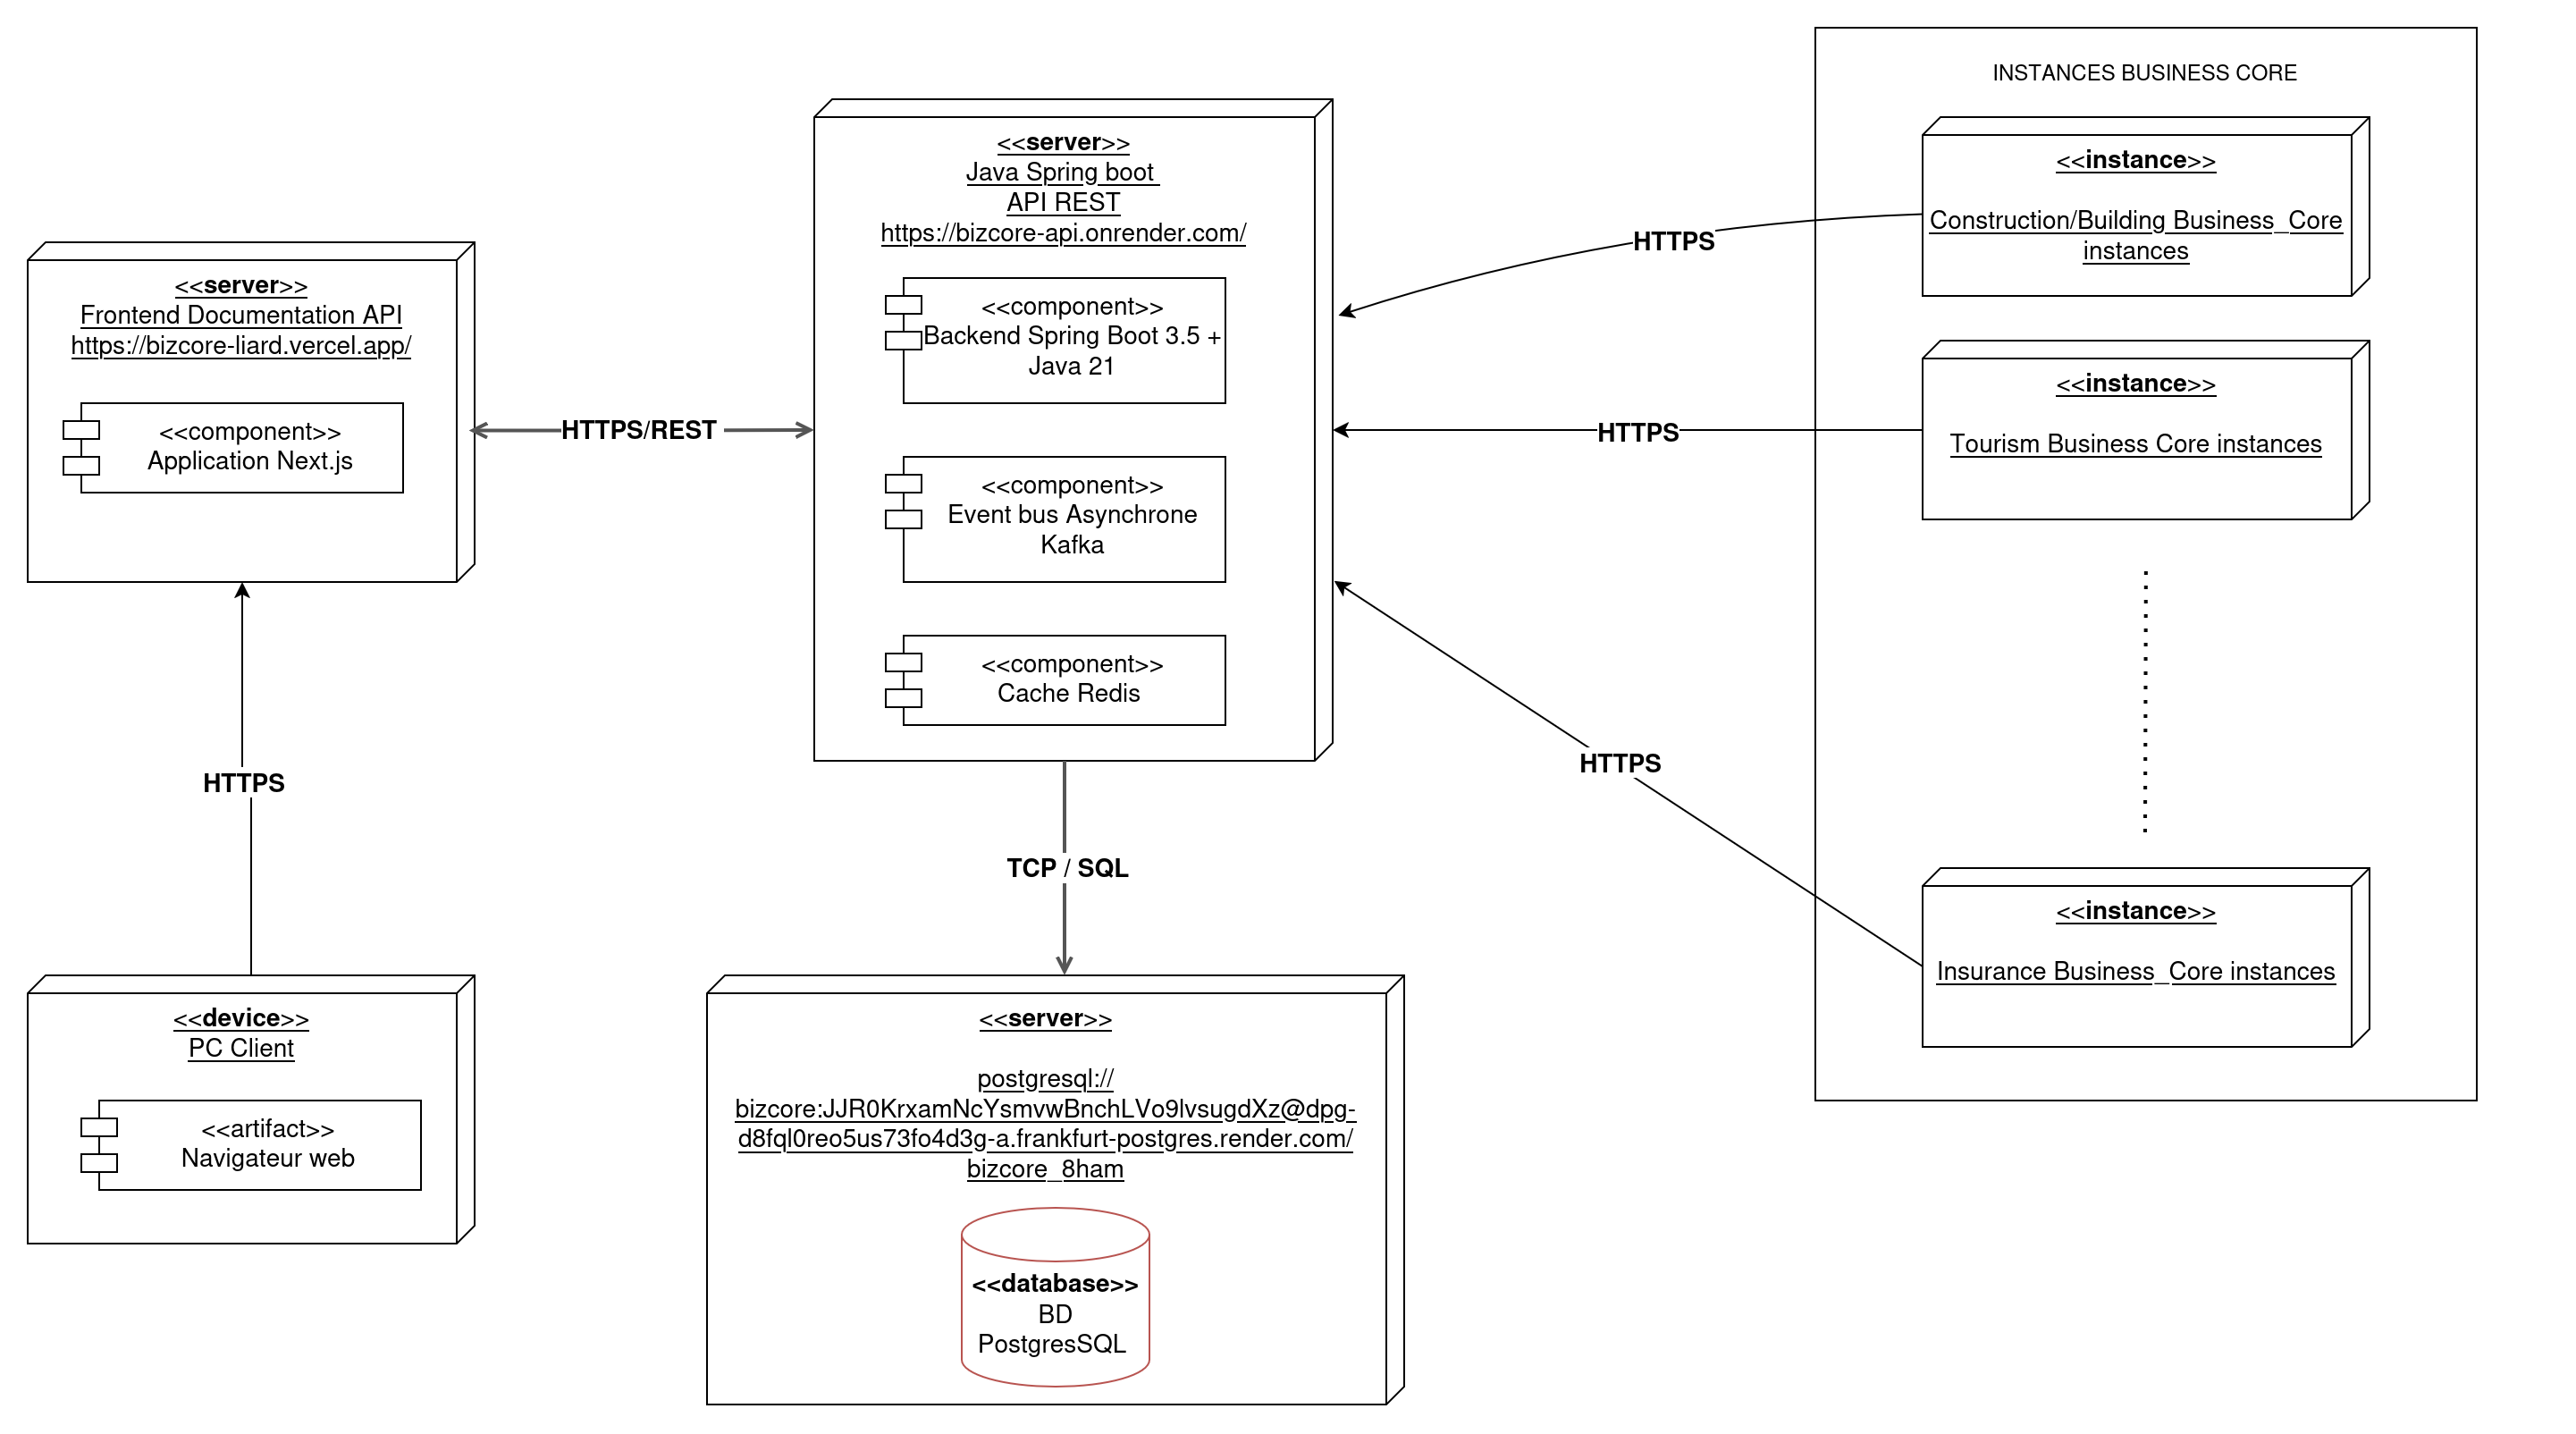
\includegraphics[width=\linewidth]{figures/diagrammes/DEPLOIEMENT.drawio.png}
   \captionof{figure}{Diagramme de déploiement du système}
    \label{fig:deploy}
\end{figure}
\label{fig:deploy} 

\begin{figure}[htbp]
  \centering
  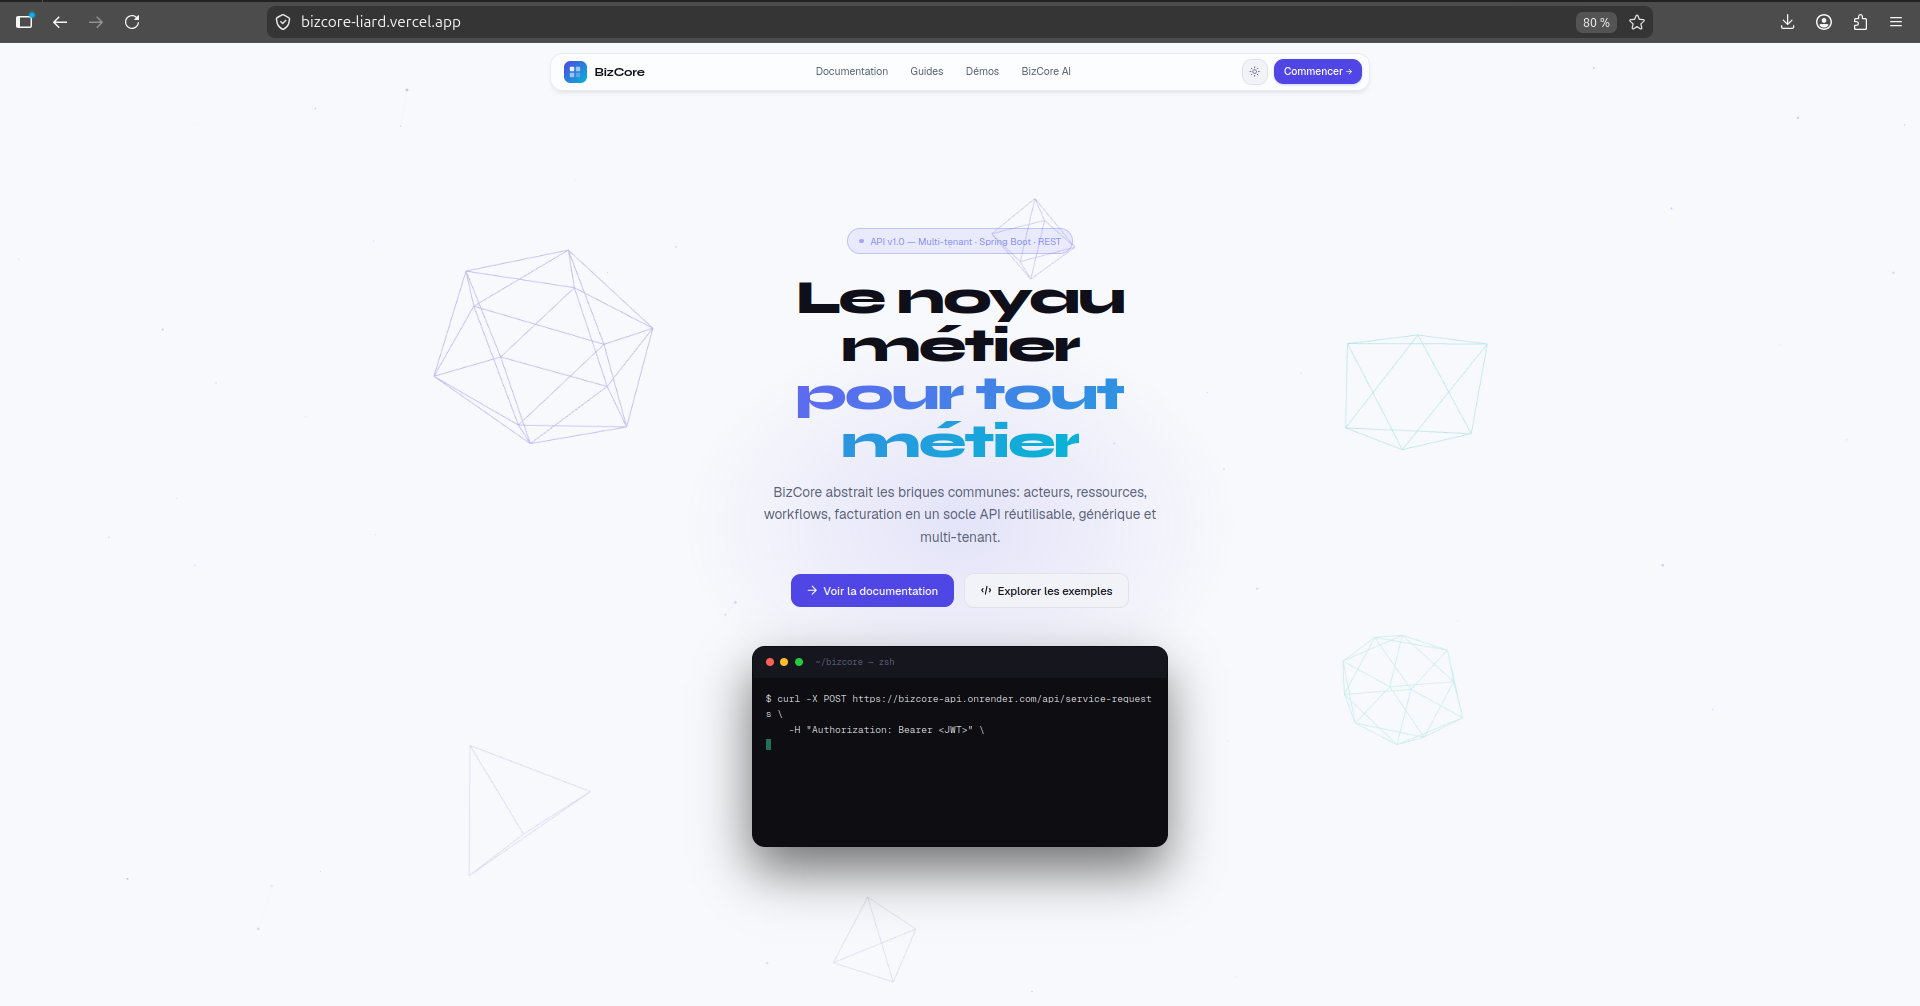
\includegraphics[width=0.95\textwidth]{figures/Screenshots/VITRINE.png}
  \caption{Page d'accueil du site vitrine déployé sur Vercel}
  \label{fig:front-home}
\end{figure}

\begin{figure}[htbp]
  \centering
  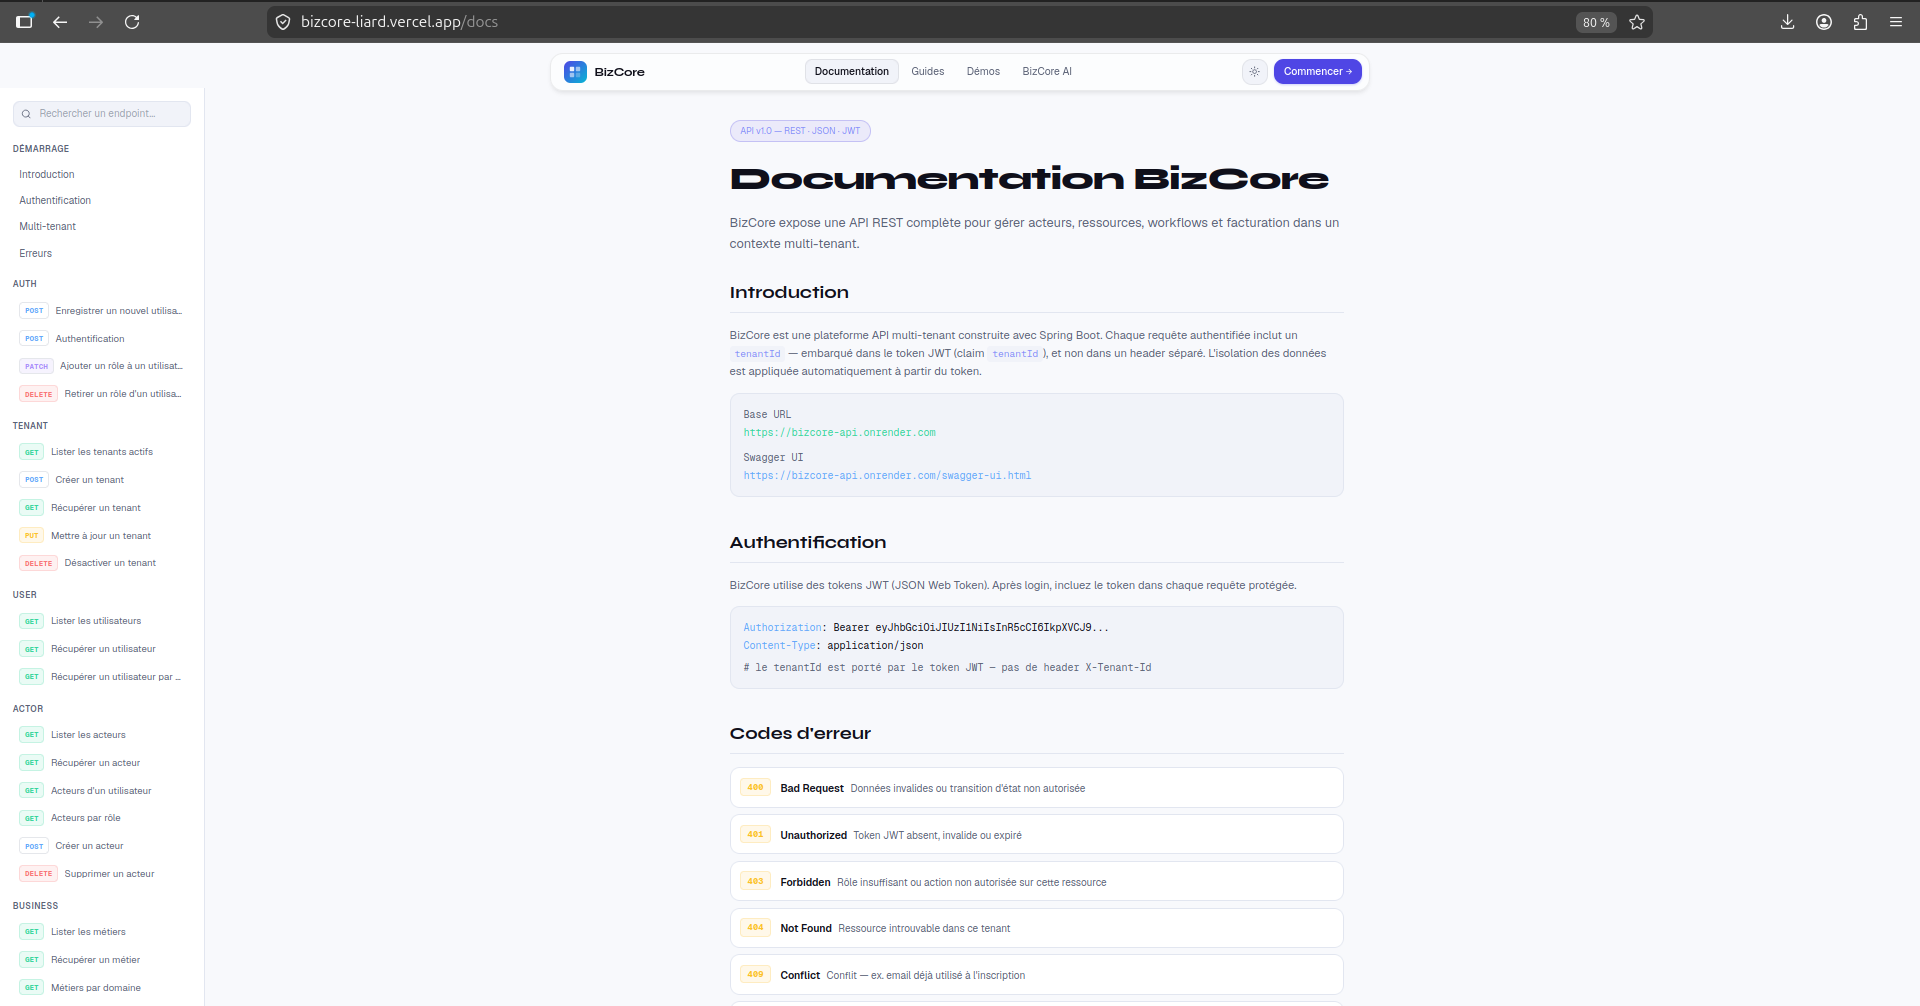
\includegraphics[width=0.95\textwidth]{figures/Screenshots/DOCUMENTATION.png}
  \caption{Documentation interactive de l'API}
  \label{fig:front-docum}
\end{figure}
 
% ============================================================
%  CHAPITRE 12 — Tests et validation
%  À inclure dans le document principal avec :
%    \input{chapitre12}   ou   \include{chapitre12}
% ============================================================

\chapter{Tests et validation}
\label{chap:tests-validation}

La qualité d'un système logiciel ne se décrète pas~: elle se démontre. Ce chapitre
présente l'ensemble de la démarche de validation mise en œuvre pour BCaaS, depuis la
stratégie globale de test jusqu'au scénario de validation bout-en-bout, en passant par
les critères d'acceptation formels. L'objectif est de montrer que chaque brique du système
--- sécurité, logique métier, isolation multi-tenant, génération de factures --- a été
vérifiée de manière systématique et reproductible.

% ------------------------------------------------------------
\section{Stratégie de test}
\label{sec:strategie-test}

% ---- 12.1.1 ------------------------------------------------
\subsection{Vue d'ensemble et outillage}
\label{subsec:outillage}

La validation de BCaaS repose sur \textbf{16~classes de test} totalisant
\textbf{152~méthodes}, organisées selon une pyramide de test à trois niveaux. L'ensemble
du dispositif s'appuie sur la stack de test standard de l'écosystème Spring~Boot~:

\begin{description}[leftmargin=0.5cm]
  \item[\textbf{JUnit~5} (\textit{Jupiter})]
    Socle d'exécution des tests~: annotations \texttt{@Test}, \texttt{@BeforeEach},
    \texttt{@AfterEach}, \texttt{@ParameterizedTest}. JUnit~5 apporte la prise en charge
    des extensions (\texttt{@ExtendWith}), utilisée notamment pour injecter le contexte
    Spring ou Mockito.

  \item[\textbf{Mockito}]
    Bibliothèque de création de \textit{mocks} et de \textit{stubs}. Elle permet de
    simuler les dépendances externes d'un composant (repositories, services tiers) afin de
    tester la logique d'un service en totale isolation, sans base de données réelle ni
    appel réseau.

  \item[\textbf{AssertJ}]
    Bibliothèque d'assertions fluides (\texttt{assertThat(...).isEqualTo(...)},
    \texttt{.contains(...)}, \texttt{.isNotNull()}...). Sa syntaxe chaînée améliore la
    lisibilité des assertions et produit des messages d'erreur plus explicites que les
    assertions JUnit natives.

  \item[\textbf{spring-boot-starter-test}]
    Méta-dépendance qui embarque JUnit~5, Mockito et AssertJ, ainsi que
    \texttt{MockMvc} pour les tests de contrôleurs HTTP et \texttt{@SpringBootTest} pour
    les tests d'intégration avec contexte Spring complet.

  \item[\textbf{spring-security-test}]
    Extension dédiée aux tests de la couche de sécurité Spring Security. Elle fournit les
    annotations \texttt{@WithMockUser} et \texttt{@WithUserDetails}, ainsi que les
    utilitaires \texttt{SecurityMockMvcRequestPostProcessors} pour simuler des requêtes
    authentifiées sans générer de vrais tokens JWT.
\end{description}

% ---- 12.1.2 ------------------------------------------------
\subsection{Environnement de test}
\label{subsec:env-test}

Les tests s'exécutent dans un environnement entièrement isolé de la base de données de
production ou de développement. Deux choix techniques fondamentaux garantissent cette
isolation~:

\paragraph{Base H2 en mémoire.}
H2 est un moteur de base de données relationnelle embarqué, écrit en Java, qui s'exécute
entièrement en mémoire vive (\textit{in-memory}). Il n'est pas nécessaire d'installer ni
de démarrer un serveur de base de données externe~: H2 démarre automatiquement avec le
contexte Spring et s'arrête à la fin de la suite de tests. La configuration
\texttt{ddl-auto=create-drop} garantit que le schéma est recréé à chaque lancement et
détruit à la fin, rendant chaque exécution de tests parfaitement reproductible et
indépendante de l'état laissé par une exécution précédente.

\paragraph{Liquibase désactivé.}
En production et en développement, BCaaS utilise Liquibase pour gérer les migrations de
schéma de façon versionnée. Liquibase est désactivé dans le profil de test~: le schéma est
entièrement reconstruit par Hibernate à partir des entités JPA (\texttt{create-drop}), ce
qui garantit que les tests ne dépendent pas d'un état de migration particulier et
s'exécutent aussi bien sur la première version que sur une version ultérieure du schéma.

\paragraph{Profil Spring dédié.}
Un profil Spring \texttt{test} est activé pour les tests d'intégration. Ce profil
surcharg les propriétés de connexion (\texttt{spring.datasource.url=jdbc:h2:mem:testdb}),
désactive les mécanismes de cache, et configure des secrets JWT simplifiés adaptés à
l'environnement de test.

% ---- 12.1.3 ------------------------------------------------
\subsection{Les trois niveaux de test}
\label{subsec:niveaux-test}

La stratégie de test de BCaaS suit le principe de la \textbf{pyramide de test}~: une large
base de tests unitaires rapides, une couche intermédiaire de tests de contrôleurs, et un
sommet de tests d'intégration plus lents mais plus représentatifs du comportement réel du
système.

\subsubsection*{Niveau 1 — Tests unitaires de services}

Les tests unitaires ciblent la \textbf{logique métier pure} des services applicatifs, en
isolation complète de toute infrastructure. Toutes les dépendances (repositories,
services tiers) sont remplacées par des mocks Mockito.

Les services couverts sont~:

\begin{itemize}
  \item \textbf{InvoiceService}~: génération automatique de facture lors de la transition
        \texttt{fulfill}, calcul des montants, association à la demande de service et au
        tenant.
  \item \textbf{BusinessService}~: création, modification et suppression de métiers~;
        vérification des règles de nommage et d'unicité au sein d'un tenant.
  \item \textbf{TenantService}~: provisionnement d'un nouveau tenant, vérification de
        l'absence de doublon, initialisation des configurations par défaut.
  \item \textbf{ActorService}~: gestion du cycle de vie des acteurs (prestataires, clients)
        et de leurs rôles au sein d'un tenant.
  \item \textbf{ServiceRequestService}~: machine à états de la demande de service~;
        validation des transitions autorisées et déclenchement des effets de bord
        (notification, facturation).
  \item \textbf{ServiceCatalogueService}~: gestion des services offerts par un métier~;
        règles de visibilité et de tarification.
  \item \textbf{BusinessRuleService}~: évaluation des règles métier configurables par
        tenant~; vérification de la conformité des demandes aux politiques en vigueur.
  \item \textbf{TenantContextTest}~: vérification du bon fonctionnement du mécanisme de
        propagation du \texttt{tenant\_id} dans le contexte de thread (ThreadLocal)~; test
        des cas de corruption ou d'absence de contexte.
\end{itemize}

\subsubsection*{Niveau 2 — Tests de contrôleurs (WebMvc)}

Les tests de contrôleurs utilisent \texttt{MockMvc}, qui simule des requêtes HTTP sans
démarrer un vrai serveur web. Le contexte Spring est chargé partiellement
(\texttt{@WebMvcTest}), incluant uniquement la couche web (contrôleurs, filtres,
sérialiseurs JSON) et excluant la couche de persistance.

Les services sont mockés via \texttt{@MockBean}, ce qui permet de se concentrer sur~:

\begin{itemize}
  \item la \textbf{désérialisation} des corps de requêtes JSON et la validation des
        contraintes (\texttt{@Valid}, \texttt{@NotNull}, tailles, formats)~;
  \item le \textbf{routage} des URLs vers les bonnes méthodes de contrôleur~;
  \item la \textbf{sérialisation} des réponses JSON et les codes HTTP retournés (200, 201,
        400, 403, 404, 409)~;
  \item la \textbf{gestion des erreurs} via les \texttt{@ExceptionHandler} et le
        \texttt{ControllerAdvice} global.
\end{itemize}

Les contrôleurs couverts sont \textbf{BusinessController}, \textbf{InvoiceController},
\textbf{ActorController} et \textbf{ServiceRequestController}.

\subsubsection*{Niveau 3 — Tests de sécurité et d'intégration}

Ce niveau constitue le sommet de la pyramide~: les tests chargent le contexte Spring
complet (\texttt{@SpringBootTest}) avec la base H2 en mémoire, et exercent le système
de bout en bout à travers plusieurs couches.

\begin{description}[leftmargin=0.5cm]
  \item[\textbf{JwtServiceTest}]
    Vérifie la génération, la signature et la validation des tokens JWT~: format du token,
    présence et valeur des \textit{claims} (\texttt{sub}, \texttt{tenantId}, \texttt{exp},
    \texttt{iat}), rejet des tokens expirés ou falsifiés, et extraction correcte du
    \texttt{tenantId} depuis le token.

  \item[\textbf{SecurityIntegrationTest}]
    Teste le filtre de sécurité sur l'ensemble des endpoints protégés~: rejet des requêtes
    sans token (401), rejet des tokens invalides (401), autorisation correcte des requêtes
    avec un token valide, et vérification que les endpoints publics (inscription, connexion)
    sont bien accessibles sans authentification.

  \item[\textbf{ServiceRequestIntegrationTest}]
    Scénario d'intégration complet de la demande de service~: création d'un contexte tenant,
    d'un acteur demandeur et d'un prestataire, d'un service au catalogue, émission d'une
    demande, puis parcours de toutes les transitions de la machine à états
    (\texttt{pending} → \texttt{accepted} → \texttt{in\_progress} → \texttt{fulfilled})
    avec vérification, à chaque étape, de l'état persisté en base et de la génération
    automatique de la facture lors du passage à \texttt{fulfilled}.
\end{description}

% ------------------------------------------------------------
\section{Critères d'acceptation}
\label{sec:criteres-acceptation}

% ---- 12.2.1 ------------------------------------------------
\subsection{Définition et méthode}
\label{subsec:criteres-def}

Les critères d'acceptation formalisent les conditions minimales que BCaaS doit satisfaire
pour être considéré comme livrable. Chaque critère est identifié par un code
\texttt{ACC-XXX}, formulé de manière vérifiable et associé à une méthode de vérification
concrète. Cette approche s'inspire des pratiques de \textit{Behavior-Driven Development}
(BDD) et garantit que la validation n'est pas subjective~: un critère est soit satisfait,
soit non satisfait, sans ambiguïté.

% ---- 12.2.2 ------------------------------------------------
\subsection{Tableau des critères}
\label{subsec:criteres-tableau}

\begin{table}[ht]
  \centering
  \caption{Critères d'acceptation et méthodes de vérification}
  \label{tab:criteres-acceptation}
  \renewcommand{\arraystretch}{1.4}
  \begin{tabularx}{\textwidth}{>{\bfseries}p{1.8cm}
                               >{\raggedright\arraybackslash}X
                               >{\raggedright\arraybackslash}p{4.2cm}}
    \toprule
    \textbf{ID} & \textbf{Critère} & \textbf{Méthode de vérification} \\
    \midrule
    ACC-001 & Les endpoints REST répondent correctement aux requêtes valides et retournent
              les codes HTTP appropriés (2xx, 4xx) pour les cas d'erreur.
            & Tests WebMvc + validation manuelle via Swagger UI \\
    ACC-002 & L'authentification par JWT fonctionne~: génération, signature, validation et
              rejet des tokens expirés ou malformés.
            & \texttt{JwtServiceTest}, \texttt{SecurityIntegrationTest} \\
    ACC-003 & Le cycle complet CdS $\rightarrow$ FdS (demande de service à facture) se
              déroule sans erreur à travers toutes les transitions de la machine à états.
            & \texttt{ServiceRequestIntegrationTest} \\
    ACC-004 & La facture est générée automatiquement lors du passage à l'état
              \texttt{fulfilled}, avec les montants et références corrects.
            & Test de service \texttt{InvoiceServiceTest} + vérification en base H2 \\
    ACC-005 & L'isolation multi-tenant est garantie~: un tenant ne peut accéder aux données
              d'un autre, même en cas de manipulation du token.
            & \texttt{TenantContextTest} + \texttt{SecurityIntegrationTest} \\
    ACC-006 & La documentation Swagger (OpenAPI) est à jour et reflète fidèlement tous les
              endpoints exposés.
            & Validation visuelle sur \texttt{/swagger-ui.html} \\
    \bottomrule
  \end{tabularx}
\end{table}

% ---- 12.2.3 ------------------------------------------------
\subsection{Analyse des critères}
\label{subsec:criteres-analyse}

\paragraph{ACC-001 — Endpoints REST.}
Ce critère couvre la surface d'API complète de BCaaS. Les tests WebMvc vérifient
systématiquement les cas nominaux (requête valide $\rightarrow$ réponse 200/201) et les
cas d'erreur les plus fréquents~: corps de requête invalide (400), ressource inexistante
(404), conflit d'identifiant (409), et accès non autorisé (403). La validation manuelle
via Swagger UI complète ces tests automatisés en permettant une exploration visuelle
des contrats d'API.

\paragraph{ACC-002 — Authentification JWT.}
La sécurité de BCaaS repose entièrement sur les JWT~: chaque requête vers un endpoint
protégé doit porter un token valide, signé avec la clé secrète du serveur, non expiré, et
contenant un \texttt{tenantId} cohérent avec les données demandées. Les tests de ce critère
couvrent le chemin nominale (token valide $\rightarrow$ accès accordé) et les cas
d'attaque les plus courants (token absent, expiré, signature altérée, \texttt{tenantId}
modifié).

\paragraph{ACC-003 — Cycle CdS $\rightarrow$ FdS.}
Ce critère valide le flux métier central de BCaaS. CdS désigne la \textit{Commande de
Service} (demande émise par un client) et FdS la \textit{Facture de Service} générée à
l'issue de la prestation. Le test d'intégration associé parcourt toutes les transitions de
la machine à états et vérifie à chaque étape que~: (i) la transition est acceptée ou
refusée conformément aux règles métier, (ii) l'état persisté en base est correct, et (iii)
les effets de bord attendus (notifications, génération de facture) sont bien déclenchés.

\paragraph{ACC-004 — Génération automatique de la facture.}
La facture est le document qui matérialise la fin d'une prestation et déclenche le
processus de paiement. Sa génération automatique à l'état \texttt{fulfilled} est un
invariant métier critique~: aucune prestation ne doit pouvoir être marquée comme terminée
sans qu'une facture valide soit créée. Les tests vérifient également que les montants
calculés correspondent aux tarifs du catalogue et que les références croisées
(identifiant de la demande, identifiant du tenant, identifiant du prestataire) sont
correctement renseignées.

\paragraph{ACC-005 — Isolation multi-tenant.}
L'isolation multi-tenant est à la fois un critère de sécurité et un critère de conformité.
\texttt{TenantContextTest} vérifie que le mécanisme de propagation du \texttt{tenant\_id}
par ThreadLocal fonctionne correctement dans tous les cas~: contexte présent, contexte
absent, changement de contexte entre deux requêtes. \texttt{SecurityIntegrationTest}
complète cette vérification en s'assurant qu'un token portant un \texttt{tenantId} A ne
permet pas d'accéder aux ressources d'un tenant B.

\paragraph{ACC-006 — Documentation Swagger.}
La documentation Swagger (générée via SpringDoc/OpenAPI~3) constitue le contrat d'API
exposé aux développeurs consommateurs de BCaaS. Sa validité est vérifiée manuellement~:
chaque endpoint documenté est testé via l'interface Swagger UI pour s'assurer que les
paramètres, les corps de requête et les réponses décrits correspondent au comportement
réel de l'API.

% ------------------------------------------------------------
\section{Scénario de validation bout-en-bout}
\label{sec:scenario-e2e}

% ---- 12.3.1 ------------------------------------------------
\subsection{Objectif et portée}
\label{subsec:e2e-objectif}

Le scénario de validation bout-en-bout constitue la démonstration de référence de BCaaS.
Son objectif est de valider, en une seule séquence cohérente, l'ensemble des mécanismes
fondamentaux du système~: authentification JWT, isolation multi-tenant, machine à états
de la demande de service, et génération automatique de facture. Ce scénario est conçu
pour être reproductible aussi bien par les tests automatisés (\texttt{ServiceRequestIntegrationTest})
que par une démonstration manuelle lors d'une soutenance.

% ---- 12.3.2 ------------------------------------------------
\subsection{Déroulement du scénario nominal}
\label{subsec:e2e-scenario}

Le scénario se déroule en six étapes séquentielles, chacune produisant un état observable
vérifiable~:

\begin{enumerate}[leftmargin=*, label=\textbf{Étape \arabic*.}]

  \item \textbf{Inscription et connexion — obtention du JWT.}\\
    Un nouvel utilisateur s'inscrit via \texttt{POST /api/auth/register} en fournissant
    ses informations et le nom de son organisation (tenant). BCaaS provisionne
    automatiquement le tenant, crée le compte utilisateur et retourne un token JWT signé.
    Ce token contient le \texttt{tenantId} du tenant nouvellement créé et est inclus dans
    l'en-tête \texttt{Authorization: Bearer <token>} de toutes les requêtes suivantes.\\
    \textit{Vérification~:} le token est bien formé (trois segments base64 séparés par des
    points), non expiré, et le \texttt{tenantId} est présent dans les \textit{claims}.

  \item \textbf{Création d'un acteur, d'un portfolio et d'un métier.}\\
    L'utilisateur crée un acteur prestataire via \texttt{POST /api/actors}, lui associe
    un portfolio de compétences, puis crée un métier (\textit{business}) via
    \texttt{POST /api/businesses}. Ces entités sont automatiquement associées au tenant
    extrait du JWT.\\
    \textit{Vérification~:} les réponses HTTP retournent le statut 201, les entités
    créées sont récupérables via les endpoints \texttt{GET} correspondants et portent bien
    le \texttt{tenantId} attendu.

  \item \textbf{Ajout d'un service au catalogue.}\\
    Un service est ajouté au catalogue du métier via
    \texttt{POST /api/service-catalogue}. La définition du service inclut
    son libellé, sa description, son tarif unitaire et son unité de facturation.\\
    \textit{Vérification~:} le service est visible dans le catalogue du tenant via
    \texttt{GET /api/service-catalogue} et son tarif est correctement persisté.

  \item \textbf{Émission d'une demande de service (CdS).}\\
    Un acteur client émet une demande de service via
    \texttt{POST /api/service-requests}, en référençant le service du catalogue et en
    précisant les paramètres de la prestation (quantité, date souhaitée, instructions
    spécifiques). La demande est créée à l'état \texttt{PENDING}.\\
    \textit{Vérification~:} la demande est persistée avec l'état \texttt{PENDING},
    l'identifiant de la demande est retourné dans la réponse, et la demande est visible
    dans la liste des demandes du tenant.

  \item \textbf{Transitions d'état et génération de la facture.}\\
    Le prestataire fait progresser la demande à travers les transitions de la machine à
    états~:
    \begin{itemize}
      \item \texttt{PENDING} $\rightarrow$ \texttt{ACCEPTED}~: le prestataire accepte la
            demande via \texttt{PATCH /api/service-requests/\{id\}/accept}.
      \item \texttt{ACCEPTED} $\rightarrow$ \texttt{IN\_PROGRESS}~: le prestataire démarre
            la prestation via \texttt{PATCH /api/service-requests/\{id\}/start}.
      \item \texttt{IN\_PROGRESS} $\rightarrow$ \texttt{FULFILLED}~: le prestataire
            marque la prestation comme terminée via
            \texttt{PATCH /api/service-requests/\{id\}/fulfill}.
    \end{itemize}
    Lors du passage à \texttt{FULFILLED}, BCaaS génère automatiquement une facture
    (FdS) associée à la demande. Cette génération constitue l'\textbf{accusé de réception
    métier}~: elle matérialise la fin de la prestation et déclenche le processus de
    paiement.\\
    \textit{Vérification~:} après chaque transition, l'état persisté est contrôlé. Après
    \texttt{fulfill}, la facture est récupérable via \texttt{GET /api/invoices} et ses
    montants correspondent au tarif du catalogue multiplié par la quantité de la demande.

  \item \textbf{Paiement de la facture.}\\
    L'acteur client enregistre le paiement de la facture via
    \texttt{PATCH /api/invoices/\{id\}/pay}. La facture passe à l'état \texttt{PAID}
    et la demande de service est clôturée.\\
    \textit{Vérification~:} la facture est à l'état \texttt{PAID}, la date de paiement
    est renseignée, et aucune transition supplémentaire n'est acceptée par la machine à
    états (idempotence du paiement).

\end{enumerate}

% ---- 12.3.3 ------------------------------------------------
\subsection{Ce que le scénario valide}
\label{subsec:e2e-validation}

Ce parcours en six étapes exerce simultanément les mécanismes les plus critiques de
BCaaS~:

\begin{description}[leftmargin=0.5cm]
  \item[\textbf{La machine à états de la demande de service}]
    Chaque transition est validée~: les transitions autorisées aboutissent, les transitions
    interdites sont rejetées avec un code HTTP~409. L'ordre des transitions est imposé par
    la machine à états et ne peut pas être contourné via l'API.

  \item[\textbf{L'isolation multi-tenant}]
    Toutes les entités créées (acteurs, métiers, services, demandes, factures) sont
    automatiquement scopées au tenant du JWT. Un deuxième tenant créé en parallèle ne
    voit aucune de ces données.

  \item[\textbf{La génération automatique de facture}]
    La facture est créée de façon atomique avec la transition \texttt{fulfill}~: les deux
    opérations font partie de la même transaction JPA, garantissant qu'il ne peut pas
    exister de demande \texttt{FULFILLED} sans facture associée.

  \item[\textbf{La cohérence des références croisées}]
    La facture référence correctement la demande, le prestataire, le client et le tenant.
    Ces références sont vérifiées via des assertions sur les identifiants retournés par
    les différents endpoints.
\end{description}

% ------------------------------------------------------------
\section{Note sur la couverture de code et perspectives}
\label{sec:couverture}

% ---- 12.4.1 ------------------------------------------------
\subsection{État actuel}
\label{subsec:couverture-actuel}

Aucun outil de mesure de couverture de code (\textit{code coverage}) n'est actuellement
intégré au pipeline de build de BCaaS. Les 152~tests constituent néanmoins une base de
non-régression substantielle qui couvre~:

\begin{itemize}
  \item l'ensemble des chemins nominaux de tous les services métier~;
  \item les principaux cas d'erreur et cas limites identifiés durant le développement~;
  \item le cycle de vie complet de la demande de service, de l'émission au paiement~;
  \item les mécanismes de sécurité (authentification, autorisation, isolation tenant).
\end{itemize}

En l'absence de mesure formelle, il est impossible d'affirmer un taux de couverture précis.
Cependant, la couverture fonctionnelle --- c'est-à-dire la proportion des fonctionnalités
métier couvertes par au moins un test --- est estimée à un niveau satisfaisant pour un MVP.

% ---- 12.4.2 ------------------------------------------------
\subsection{Perspectives d'amélioration}
\label{subsec:couverture-perspectives}

Plusieurs améliorations sont identifiées pour les versions futures de BCaaS (voir
chapitre~14)~:

\begin{description}[leftmargin=0.5cm]
  \item[\textbf{Intégration de JaCoCo}]
    JaCoCo (\textit{Java Code Coverage Library}) s'intègre nativement avec Maven et
    Gradle. Son ajout permettrait de générer un rapport de couverture à chaque build,
    d'identifier les branches non testées et de définir des seuils minimaux de couverture
    (par exemple, 80\,\% de couverture de branches) en dessous desquels le build échoue.

  \item[\textbf{Tests de mutation}]
    Les tests de mutation (avec des outils comme PIT/Pitest) permettent d'évaluer la
    \textit{qualité} des tests plutôt que leur simple existence~: ils introduisent
    délibérément des fautes dans le code (mutations) et vérifient que les tests les
    détectent. Un test qui passe même en présence d'une mutation est un test insuffisant.

  \item[\textbf{Tests de charge}]
    BCaaS étant un service multi-tenant destiné à héberger plusieurs organisations
    simultanément, des tests de charge avec des outils comme Gatling ou JMeter permettraient
    de valider les performances sous des montées en charge réalistes et d'identifier les
    goulots d'étranglement avant la mise en production.

  \item[\textbf{Tests de contrat (Consumer-Driven Contract Testing)}]
    Si BCaaS est consommé par plusieurs applications clientes, les tests de contrat
    (avec Pact, par exemple) garantiraient que les évolutions de l'API ne cassent pas
    silencieusement les consommateurs existants.
\end{description}

% ------------------------------------------------------------
\section*{Synthèse}
\addcontentsline{toc}{section}{Synthèse}
\label{sec:synthese-chap12}

Ce chapitre a présenté la démarche complète de validation de BCaaS. La stratégie de test
repose sur une pyramide à trois niveaux --- tests unitaires, tests de contrôleurs et tests
d'intégration --- mobilisant 16~classes et 152~méthodes sur un environnement H2 en mémoire
parfaitement isolé. Les six critères d'acceptation formels garantissent que les
fonctionnalités les plus critiques --- sécurité JWT, isolation multi-tenant, cycle
CdS~$\rightarrow$~FdS --- sont vérifiées de manière systématique et reproductible.

Le scénario de validation bout-en-bout constitue la démonstration de référence du système~:
en six étapes cohérentes, il exerce simultanément la machine à états, l'isolation tenant
et la génération automatique de facture, offrant une preuve d'intégration concrète et
démontrable lors de la soutenance.

L'absence de mesure formelle de couverture constitue la principale limite reconnue de ce
dispositif~; son adressage, via l'intégration de JaCoCo et de tests de mutation, figure
parmi les priorités du plan d'évolution présenté au chapitre~14.
% \chapter{Gestion de projet}
\label{chap:gestion}

\iffalse
\section{Méthodologie}

Le projet a été conduit de façon incrémentale, organisée en sprints assortis de critères de
priorité (P0 indispensable, P1 important). Chaque sprint livrait un incrément vérifiable et
faisait l'objet d'une validation avant passage au suivant : modélisation Merise et UML,
puis implémentation, puis tests automatisés et audits de code. Cette discipline a permis de
détecter et corriger tôt les erreurs de modélisation (cardinalités, périmètre des entités).

\section{Organisation des sprints}

\begin{table}[H]
\centering
\caption{Découpage en sprints}
\label{tab:sprints}
\renewcommand{\arraystretch}{1.25}\footnotesize
\begin{tabularx}{\linewidth}{L{2.4cm} X}
\toprule
\textbf{Sprint} & \textbf{Contenu} \\
\midrule
Sprint 1 & Modélisation (MCD/MLD/UML), entités JPA, repositories, services de base, migrations Liquibase \\
Sprint 2 & Sécurité JWT + RBAC, DTO, pagination, gestion globale des erreurs, devises \\
Sprint 3 & Multi-tenant (TenantContext / TenantFilter), entités Message/Notification/Audit, analytique \\
Sprint 4 & Frontend Next.js (vitrine + tableau de bord), documentation, déploiement (Render, Vercel) \\
\bottomrule
\end{tabularx}
\end{table}

\section{Répartition des tâches et participation}

Le tableau~\ref{tab:participation} présente la répartition de la contribution entre les
membres du groupe. \emph{(Les taux sont à compléter ; chacun est évalué sur 100.)}

\begin{table}[H]
\centering
\caption{Répartition de la participation}
\label{tab:participation}
\renewcommand{\arraystretch}{1.3}
\begin{tabularx}{\linewidth}{L{6cm} X C{2.6cm}}
\toprule
\textbf{Membre} & \textbf{Contributions principales} & \textbf{Participation} \\
\midrule
ETCHOME Chris           & \dotfill & \underline{\hspace{1cm}} / 100 \\
{[Membre 2 — Nom Prénom]} & \dotfill & \underline{\hspace{1cm}} / 100 \\
KENNE DIHA Lea & \dotfill & \underline{\hspace{1cm}} / 100 \\
{[Membre 4 — Nom Prénom]} & \dotfill & \underline{\hspace{1cm}} / 100 \\
MBA BELA Oceanne & \dotfill & \underline{\hspace{1cm}} / 100 \\
{[Membre 6 — Nom Prénom]} & \dotfill & \underline{\hspace{1cm}} / 100 \\
\bottomrule
\end{tabularx}
\end{table}

\section{Outils et gestion de version}

Le code est versionné sous Git (dépôt GitHub), avec un flux de branches distinguant le code
stable (\texttt{main}), l'intégration (\texttt{dev}) et les branches de fonctionnalités
(\texttt{feat/*}) ou de correction (\texttt{fix/*}). La documentation technique est rédigée
en Markdown et en \LaTeX{} (le présent rapport).
\fi

\chapter{Perspectives d'amélioration}
\label{chap:perspectives}

Le MVP livré pose des fondations solides ; il ouvre néanmoins de nombreuses pistes
d'amélioration, dont plusieurs correspondent aux contraintes technologiques avancées du
sujet. Cette feuille de route est organisée par horizon.

\section{Court terme : finalisation des briques posées}

\begin{itemize}
  \item \textbf{Câblage de l'événementiel Kafka.} L'infrastructure (producteur configuré,
        topic \texttt{bizcore.events}, consommateur de notifications) est en place ; il
        reste à publier effectivement les événements de domaine (changement de statut d'une
        demande, génération de facture) pour rendre la chaîne pleinement \emph{event-driven}.
  \item \textbf{Activation du cache Redis.} Le gestionnaire de cache et les TTL sont
        définis ; l'ajout d'annotations \texttt{@Cacheable} / \texttt{@CacheEvict} sur les
        lectures fréquentes (règles métier, configuration tenant, catalogue) activerait le
        cache déjà préfixé par tenant.
  \item \textbf{Limitation de débit (rate limiting).} La dépendance Bucket4j est présente ;
        son intégration permettrait d'appliquer des quotas par tenant, prolongeant l'analogie
        de la bande passante et de la QoS.
  \item \textbf{Mesure de couverture de tests.} L'ajout de JaCoCo fournirait un indicateur
        chiffré de couverture.
    \item\textbf{Sur le plan de l'architecture: }il s'agirait d'étendre la couverture des cent cinquante-deux tests automatisés afin d'inclure des scénarios de charge et des tests d'intégration multitenant plus poussés, garantissant la robustesse de l'isolation par tenantId dans des conditions de concurrence élevée
    
    \item\textbf{La documentation OpenAPI: }pourrait également être enrichie d'exemples d'utilisation et de scénarios d'erreur, facilitant l'adoption de l'API par de nouveaux développeurs

    \item\textbf{le service d'analytique et la piste d'audit:} pourraient être complétés par des tableaux de bord de supervision en temps réel, exploitant les données déjà collectées pour offrir une visibilité immédiate sur l'activité de chaque tenant
    
\end{itemize}

\section{Moyen terme : robustesse et qualité de service}

\begin{itemize}
  \item \textbf{Isolation multi-tenant renforcée.} Passer de la discipline applicative à
        une barrière systématique au moyen d'un filtre Hibernate \texttt{@Filter} ou de la
        \emph{Row-Level Security} PostgreSQL, voire d'une isolation par schéma dédié pour
        les tenants premium.
  \item \textbf{QoS différenciée.} Introduire des niveaux de service inspirés de DiffServ
        (Bronze, Silver, Gold, Platinum) combinant priorité, latence cible et stratégie
        d'isolation.
  \item \textbf{Observabilité complète.} Exposer des métriques via Prometheus et un tableau
        de bord Grafana, et mettre en place des logs structurés agrégés.

  \item \textbf{Le modele generique}pourrait être étendu pour couvrir de nouveaux domaines métier au-delà du cas d'usage initial, validant ainsi la généricité réelle du Business Core sur des secteurs d'activité variés (santé, transport, logistique)

  \item \textbf{L'authentification JWT et le contrôle d'accès basé sur les rôles :} pourraient évoluer vers une gestion plus fine des permissions, avec la possibilité pour chaque tenant de définir ses propres rôles et politiques d'autorisation sans intervention sur le code du système
\end{itemize}

\section{Long terme : montée en charge et nouvelles contraintes}

\begin{itemize}
  \item \textbf{Architecture réactive.} Migration vers Spring WebFlux + R2DBC pour un
        modèle non bloquant, mieux adapté à une forte concurrence.
  \item \textbf{Géo-référencement natif.} Intégration de PostGIS et d'attributs de
        localisation pour les recherches géo-spatiales (\emph{geolocation aware}).
  \item \textbf{Stockage d'objets.} Adoption de MinIO pour les médias, au lieu de la simple
        URL actuellement stockée.
  \item \textbf{Sécurité renforcée.} Double authentification (2FA) et migration vers
        OAuth 2.0.
  \item \textbf{Front offline-first et international.} Transformation du frontend en PWA
        installable, mode hors-ligne, et internationalisation (i18n) web et mobile.
  \item \textbf{Application mobile native.} Client React Native partageant l'API.
  \item \textbf{Microservices.} Extraction progressive des modules en services déployés
        indépendamment, le découpage actuel ayant été pensé pour cette évolution.
  \item \textbf{Marketplace d'instances.} À terme, permettre à des entreprises de déployer
        leur propre configuration BCaaS sans développement, comme socle d'un écosystème
        d'instances métier.
  \item \textbf{ La grille de lecture protocolaire en cinq couches : }, actuellement formalisée et reliée au modèle OSI, pourrait servir de fondement à une véritable spécification ouverte du Business Core as a Service, documentée et partagée, permettant à d'autres équipes de contribuer à son évolution ou de l'adopter comme standard interne
\end{itemize}

\chapter{Conclusion générale}
\label{chap:conclusion}

\section{Bilan}

Ce projet a démontré qu'une analogie rigoureuse entre l'ingénierie des protocoles réseaux
et la conception d'une plateforme métier n'est pas une simple métaphore pédagogique :
elle constitue une véritable méthode de conception. Les concepts de couches,
d'encapsulation, de routage, d'adressage, de qualité de service et de séparation des plans
de contrôle et de données ont guidé chaque décision architecturale de BCaaS.

Les réalisations principales sont :
\begin{itemize}
  \item une grille de lecture protocolaire en cinq couches, formellement reliée au modèle
        OSI ;
  \item un modèle de données générique de quinze entités, configurable par tenant et
        implémenté sur PostgreSQL avec Liquibase ;
  \item une API REST d'environ quatre-vingt-cinq endpoints, documentée par OpenAPI et
        validée par cent cinquante-deux tests automatisés ;
  \item une authentification JWT multi-tenant avec contrôle d'accès basé sur les rôles, et
        une isolation par colonne \texttt{tenant\_id} pilotée par un contexte
        \texttt{ThreadLocal} ;
  \item un protocole d'échange formalisé pour un cas métier concret ;
  \item une piste d'audit et un service d'analytique pour la traçabilité ;
  \item un frontend Next.js (site vitrine et tableau de bord), l'ensemble étant déployé sur
        le cloud (Render et Vercel).
\end{itemize}

\section{Limites}

Le périmètre livré est celui d'un MVP. Plusieurs briques avancées du sujet sont posées mais
non pleinement câblées (événementiel Kafka, cache Redis par annotations, limitation de
débit) ou restent à venir (réactif, géo-référencement, stockage objet, 2FA, PWA/offline,
i18n, mobile natif).\\
Par ailleurs, la couverture des tests automatisés, bien que substantielle, reste centrée sur la validation fonctionnelle de l'API et n'inclut pas encore de tests de charge approfondis permettant d'évaluer le comportement du système face à un grand nombre de tenants simultanés. Enfin, le contrôle d'accès basé sur les rôles, bien qu'opérationnel, demeure relativement statique : chaque tenant ne dispose pas encore de la capacité à définir ses propres rôles et politiques d'autorisation de façon autonome.\\
Ces limites, assumées et documentées, font l'objet de la feuille de route du chapitre~\ref{chap:perspectives}.\\
\section{Apports personnels}

Ce projet a permis d'acquérir des compétences concrètes en architecture logicielle
distribuée, en conception d'API REST professionnelle, en sécurité applicative (JWT, RBAC),
en isolation multi-tenant et en modélisation de systèmes génériques. Au-delà des
technologies, la démarche de \emph{pensée protocolaire} --- définir les contrats avant le
code, modéliser les échanges comme des messages --- constitue un réflexe d'ingénieur
directement transposable à tout projet de système d'information.

Ce travail a également renforcé notre capacité à raisonner en termes de systèmes complets plutôt qu'en fonctionnalités isolées, en nous habituant à anticiper, dès la conception, des préoccupations transverses telles que la sécurité, la traçabilité et l'isolation des données, plutôt que de les traiter comme des ajouts tardifs. Cette approche constitue, selon nous, un acquis précieux pour notre future pratique en tant qu'ingénieurs en informatique.

%=====================  BIBLIOGRAPHIE ================================
\begin{thebibliography}{9}
\addcontentsline{toc}{chapter}{Bibliographie}

\bibitem{djotio}
Pr. Dr Ing. Thomas Djotio Ndié,
\emph{Cours d'Introduction aux Réseaux Locaux}, 3GI, ENSPY, 2025-2026.

\bibitem{iso7498}
ISO/IEC 7498-1,
\emph{Information technology --- Open Systems Interconnection --- Basic Reference Model},
ISO, 1994.

\bibitem{hexagonal}
A. Cockburn,
\emph{Hexagonal Architecture (Ports and Adapters)}, 2005.

\bibitem{ddd}
E. Evans,
\emph{Domain-Driven Design: Tackling Complexity in the Heart of Software},
Addison-Wesley, 2003.

\bibitem{jwt}
M. Jones, J. Bradley, N. Sakimura,
\emph{RFC 7519 --- JSON Web Token (JWT)}, IETF, 2015.

\bibitem{}\url{https://www.access-it.fr/actualite/quest-ce-quune-application-metier/}

\bibitem{strategies}
AWS Whitepaper,
\emph{SaaS Tenant Isolation Strategies: Isolating
Resources in a Multi-Tenant Environment}, 
\url{https://docs.aws.amazon.com/pdfs/whitepapers/latest/saas-tenant-isolation-strategies/saas-tenant-isolation-strategies.pdf}, 

\bibitem{nist}
Peter Mell Timothy Grance
\emph{The NIST Definition of Cloud Computing}, 
\url{https://nvlpubs.nist.gov/nistpubs/legacy/sp/nistspecialpublication800-145.pdf}, 



\bibitem{hexagonale}
Architecture heaxagonale,
\url{https://thetribe.io/glossaire-architecture-hexagonale-clean-architecture/}, 


\bibitem{springboot}
Spring Boot Reference Documentation,
\url{https://docs.spring.io/spring-boot/}, 

\bibitem{springdoc}
SpringDoc OpenAPI Documentation,
\url{https://springdoc.org},  

\bibitem{nextjs}
Next.js Documentation,
\url{https://nextjs.org/docs}, 

\bibitem{multitenant}
GeeksforGeeks,
\emph{Single-Tenant vs Multi-Tenant Architecture},
\url{https://www.geeksforgeeks.org/system-design/single-tenant-vs-multi-tenant-architecture/}, 

\bibitem{multitenancy}
okta
\emph{Multi tenancy cloud },
\url{https://www.okta.com/fr-fr/identity-101/multi-tenancy-cloud/}, 
https://www.okta.com/fr-fr/identity-101/multi-tenancy-cloud/
\end{thebibliography}


%=====================  GLOSSAIRE ====================================
\chapter*{Glossaire}
\addcontentsline{toc}{chapter}{Glossaire}
\markboth{Glossaire}{Glossaire}

\begin{description}[style=nextline,leftmargin=0pt]
  \item[BaaS (Business as a Service)] Modèle fournissant des capacités métier génériques via
        une API standardisée.
  \item[Tenant] Organisation cliente disposant d'une isolation logique de ses données et
        configurations ; analogue d'un VLAN.
  \item[Multi-tenant] Architecture servant plusieurs tenants sur une infrastructure
        partagée, avec isolation de leurs données.
  \item[Actor] Rôle joué par un utilisateur dans le système : consommateur (CdS) et/ou
        fournisseur (FdS) de service.
  \item[CdS / FdS] Consommateur de Service (émetteur de la requête) / Fournisseur de Service
        (récepteur et exécutant).
  \item[Business] Métier ou profession référencé dans le système (domaine, règles, services,
        ressources).
  \item[BusinessRule] Règle métier sous forme de paire clé--valeur ; analogue du protocole.
  \item[ServiceRequest] Demande de service entre un CdS et un FdS ; analogue d'un message
        réseau, porteuse d'un \texttt{traceId}.
  \item[Invoice] Facture générée automatiquement à la finalisation ; analogue d'un accusé de
        réception (ACK).
  \item[Portfolio] Ensemble des métiers maîtrisés par un acteur (relation N:M avec Business).
  \item[FSM] Machine à états finis décrivant le cycle de vie d'une entité (ServiceRequest,
        Invoice).
  \item[JWT] Jeton signé portant l'identité, les rôles et le \texttt{tenantId} de
        l'utilisateur authentifié.
  \item[RBAC] Contrôle d'accès basé sur les rôles.
  \item[traceId / correlationId] Identifiants de flux permettant de tracer une transaction
        de bout en bout.
  \item[DTO] Objet de transfert de données découplant la représentation exposée des entités
        persistées.
  \item[Soft delete] Suppression logique préservant les données en base
        (\texttt{isActive = false}).
  \item[Control plane / Data plane] Plan de configuration (administration) / plan d'exécution
        (transactions), par analogie avec le SDN.
\end{description}


%=====================  ANNEXES ======================================
\appendix
\chapter{Annexes}
\label{chap:annexes}

\section{Liste des endpoints REST}
\label{ann:endpoints}

L'API expose environ 85 endpoints répartis sur 17 contrôleurs. Le
tableau~\ref{tab:endpoints} en donne une vue synthétique.

\renewcommand{\arraystretch}{1.2}\footnotesize
\begin{longtable}{L{3.6cm} L{10.4cm}}
\caption{Synthèse des endpoints REST}\label{tab:endpoints}\\
\toprule
\textbf{Ressource} & \textbf{Endpoints} \\
\midrule \endfirsthead
\toprule \textbf{Ressource} & \textbf{Endpoints} \\ \midrule \endhead
\texttt{/api/auth} & POST /register, POST /login, PATCH /users/\{id\}/roles, DELETE /users/\{id\}/roles \\
\texttt{/api/tenants} & GET, GET /\{id\}, POST /register, PUT /\{id\}, DELETE /\{id\} \\
\texttt{/api/users} & GET, GET /\{id\}, GET /email/\{email\} \\
\texttt{/api/actors} & GET, GET /\{id\}, GET /user/\{userId\}, GET /role/\{role\}, POST /user/\{userId\}, DELETE /\{id\} \\
\texttt{/api/businesses} & GET, POST, GET /\{id\}, GET /domain/\{domain\}, GET /search, PUT /\{id\}, DELETE /\{id\} \\
\texttt{/api/business-rules} & GET, GET /\{id\}, GET /business/\{businessId\}, POST /business/\{businessId\}, PUT /\{id\}, DELETE /\{id\} \\
\texttt{/api/service-catalogues} & GET, GET /\{id\}, GET /business/\{businessId\}, GET /available, GET /search, POST /business/\{businessId\}, PUT /\{id\}, DELETE /\{id\} \\
\texttt{/api/service-requests} & GET, GET /\{id\}, GET /consumer/\{id\}, GET /provider/\{id\}, GET /status/\{status\}, POST /consumer/\{id\}/provider/\{id\}/catalogue/\{id\}, PATCH /\{id\}/accept, /start, /fulfill, /cancel, DELETE /\{id\} \\
\texttt{/api/invoices} & GET, GET /\{id\}, GET /status/\{status\}, GET /service-request/\{id\}, POST /service-request/\{id\}, PATCH /\{id\}/pay, /cancel, DELETE /\{id\} \\
\texttt{/.../messages} & GET, POST, GET /unread-count, PATCH /read-all, DELETE /\{messageId\} \\
\texttt{/api/notifications} & GET, GET /unread-count, PATCH /\{id\}/read, PATCH /read-all, DELETE /\{id\} \\
\texttt{/api/portfolios} & GET, GET /\{id\}, GET /actor/\{id\}, POST /actor/\{id\}, PATCH /\{id\}/businesses/\{bid\}, DELETE /\{id\}/businesses/\{bid\}, DELETE /\{id\} \\
\texttt{/api/resources} & GET, GET /\{id\}, GET /business/\{id\}, POST /business/\{id\}, PUT /\{id\}, DELETE /\{id\} \\
\texttt{/api/media} & GET, GET /\{id\}, GET /business/\{id\}, GET /type/\{type\}, POST /business/\{id\}, PUT /\{id\}, DELETE /\{id\} \\
\texttt{/api/currencies} & GET, GET /validate/\{code\} \\
\texttt{/api/analytics} & GET /tenants/\{tenantId\}/kpis \\
\texttt{/api/audit} & GET /service-requests/\{id\}, GET /actors/\{id\}, GET /trace/\{traceId\}, GET /tenants/\{id\} \\
\bottomrule
\end{longtable}

\section{Exemple de log structuré}

\begin{lstlisting}[language=json,caption={Log structuré au format JSON (proposition)},captionpos=b]
{
  "timestamp": "2025-05-04T10:05:23Z",
  "level": "INFO",
  "tenant_id": "550e8400-e29b-41d4-a716-446655440000",
  "trace_id": "7e9a8b7c-6d5e-4f3a-2b1c-9d8e7f6a5b4c",
  "actor_id": "actor_123",
  "service": "BusinessService",
  "operation": "createBusiness",
  "duration_ms": 145,
  "http_status": 201
}
\end{lstlisting}

\section{Capture Swagger UI}
\label{ann:swagger}

\begin{figure}[htbp]
  \centering
  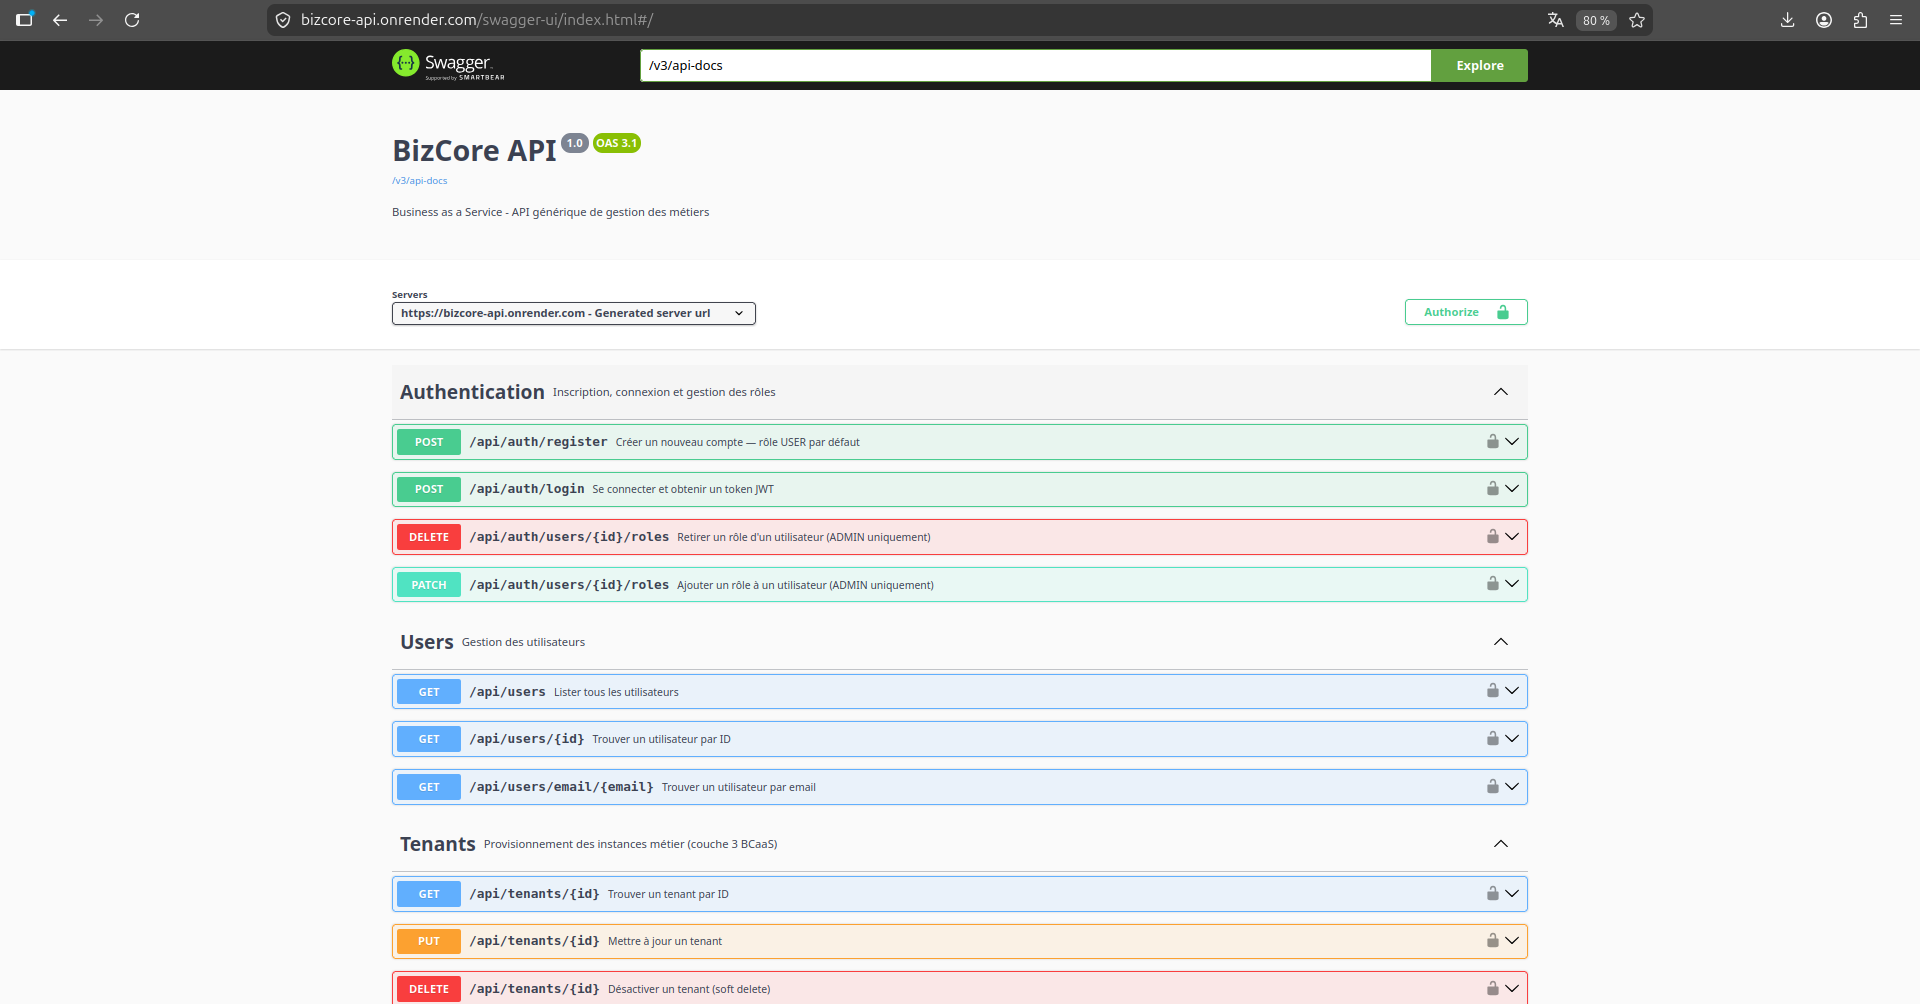
\includegraphics[width=\textwidth]{figures/Screenshots/SWAGGER.png}
  \caption{Documentation interactive Swagger UI}
  \label{fig:swagger}
\end{figure}

\section{Extraits de code significatifs}

\begin{lstlisting}[language=Java,caption={TenantContext (ThreadLocal)},captionpos=b]
public final class TenantContext {
    private static final ThreadLocal<UUID> CURRENT_TENANT = new ThreadLocal<>();
    public static void setTenantId(UUID tenantId) { CURRENT_TENANT.set(tenantId); }
    public static UUID getTenantId() { return CURRENT_TENANT.get(); }
    public static void clear() { CURRENT_TENANT.remove(); }
}
\end{lstlisting}

\begin{lstlisting}[language=Java,caption={Lecture tenant-aware dans un service},captionpos=b]
UUID tenantId = TenantContext.getTenantId();
if (tenantId != null) {
    return serviceRequestRepository.findAllByTenantId(tenantId, pageable);
}
\end{lstlisting}


\end{document}
